\documentclass[11pt,a4paper]{article}
\usepackage{type1cm}

% --- HỖ TRỢ TIẾNG VIỆT VÀ MÃ HÓA UNICODE ---
\usepackage{vntex}
\usepackage[utf8]{inputenc}
\usepackage[T5]{fontenc}
\usepackage[vietnamese]{babel}

% --- CẤU HÌNH TRANG VÀ LỀ CHUẨN ĐẠI HỌC BÁCH KHOA TP.HCM ---
\usepackage{geometry}
\geometry{
    a4paper,
    left=30mm,
    right=20mm,
    top=30mm,
    bottom=25mm,
    headheight=40pt,
    headsep=30pt,
    footskip=30pt
}

% --- KHOẢNG CÁCH DÒNG VÀ ĐOẠN VĂN ---
\usepackage{setspace}
\onehalfspacing                 % Khoảng cách dòng 1.5
\setlength{\parindent}{1.5em}    % Thụt đầu dòng đoạn văn
\setlength{\parskip}{6pt}        % Khoảng cách giữa các đoạn

% --- GÓI TOÁN HỌC & KÝ HIỆU KỸ THUẬT ---
\usepackage{amsmath,amssymb,amsfonts,amsthm}
\usepackage{bm}

% --- HÌNH ẢNH, BẢNG BIỂU & ĐỒ HỌA ---
\usepackage{graphicx}
\usepackage{booktabs}
\usepackage{array}
\usepackage{longtable}
\usepackage{tabularx}
\usepackage{xltabular}
\usepackage{multirow}
\usepackage{float}
\usepackage{caption}
\usepackage{subcaption}
\usepackage{lastpage}
\usepackage{varwidth}
\usepackage{enumitem}
\usepackage[table,xcdraw]{xcolor}
\usepackage{tikz}
\usetikzlibrary{calc,arrows,arrows.meta,positioning,shapes,shapes.multipart,fit,backgrounds,decorations.pathreplacing}

% --- PHONG CÁCH SƠ ĐỒ HỌC THUẬT (IEEE / TEXTBOOK VECTOR TIKZ) ---
\tikzset{
    acadbox/.style={
        rectangle, draw=black!85, fill=white, line width=0.75pt,
        align=center, font=\scriptsize, inner sep=4pt, minimum height=0.85cm
    },
    acadboxnav/.style={
        rectangle, draw=tablehead, fill=white, line width=0.9pt,
        align=center, font=\scriptsize, inner sep=4pt
    },
    acadhdr/.style={
        rectangle, draw=black!85, fill=black!5, line width=0.75pt,
        align=center, font=\scriptsize\bfseries, inner sep=3.5pt
    },
    acadmcu/.style={
        rectangle, draw=tablehead, fill=tablehead!4, line width=1.1pt,
        align=center, font=\footnotesize, inner sep=5pt
    },
    acadport/.style={
        rectangle, draw=black!75, fill=white, line width=0.6pt,
        align=center, font=\tiny\ttfamily, inner sep=2.2pt, minimum width=1.45cm, minimum height=0.42cm
    },
    acadzone/.style={
        rectangle, draw=black!55, dashed, line width=0.6pt,
        inner sep=7pt
    },
    acadarr/.style={-{Stealth[length=2.1mm, width=1.35mm]}, draw=black!85, line width=0.75pt},
    acadbiarr/.style={{Stealth[length=2.0mm, width=1.3mm]}-{Stealth[length=2.0mm, width=1.3mm]}, draw=black!85, line width=0.75pt},
    acadline/.style={draw=black!85, line width=0.75pt},
    acaddash/.style={-{Stealth[length=2.0mm, width=1.3mm]}, draw=tablehead, dashed, line width=0.7pt},
    acaddashbi/.style={{Stealth[length=1.9mm, width=1.25mm]}-{Stealth[length=1.9mm, width=1.25mm]}, draw=tablehead, dashed, line width=0.65pt},
    acadlbl/.style={font=\tiny\sffamily, fill=white, inner sep=1.2pt, text=black!90},
    acadpin/.style={font=\tiny\ttfamily, text=black!85},
}
\usepackage[most]{tcolorbox}

\captionsetup[figure]{labelfont={small,bf},textfont={small,it},belowskip=4pt,aboveskip=6pt}
\captionsetup[table]{labelfont={small,bf},textfont={small,it},belowskip=4pt,aboveskip=6pt}

% --- CẤU HÌNH BẢNG BIỂU CHUYÊN NGHIỆP (KHÔNG BAO GIỜ LỐ LỀ) ---
\definecolor{tablehead}{RGB}{21, 56, 96}
\definecolor{tableborder}{RGB}{165, 182, 201}
\definecolor{rowodd}{RGB}{255, 255, 255}
\definecolor{roweven}{RGB}{243, 247, 252}
\definecolor{subheadbg}{RGB}{218, 231, 245}

\newcolumntype{L}[1]{>{\raggedright\arraybackslash}p{#1}}
\newcolumntype{C}[1]{>{\centering\arraybackslash}p{#1}}
\newcolumntype{R}[1]{>{\raggedleft\arraybackslash}p{#1}}
\newcolumntype{Y}{>{\raggedright\arraybackslash}X}
\newcommand{\thcell}[1]{\textcolor{white}{\textbf{#1}}}
\setlength{\emergencystretch}{2em}
\setlength{\LTpre}{6pt}
\setlength{\LTpost}{6pt}
\setlength{\LTcapwidth}{\textwidth}

% --- LIÊN KẾT SIÊU VĂN BẢN (HYPERREF) ---
\usepackage[unicode,pdfpagelabels=false]{hyperref}
\hypersetup{
    colorlinks=true,
    linkcolor=black,
    citecolor=blue,
    urlcolor=blue,
    bookmarksnumbered=true,
    plainpages=false
}

% --- ĐỊNH DẠNG CODE LẬP TRÌNH (LISTINGS) ---
\usepackage{listings}
\definecolor{codebg}{rgb}{0.96,0.96,0.96}
\definecolor{commentgreen}{rgb}{0,0.6,0}
\definecolor{keywordblue}{rgb}{0,0,0.8}
\definecolor{stringred}{rgb}{0.8,0,0}

\lstset{
    backgroundcolor=\color{codebg},
    frame=single,
    basicstyle=\ttfamily\footnotesize,
    keywordstyle=\color{keywordblue}\bfseries,
    commentstyle=\color{commentgreen}\itshape,
    stringstyle=\color{stringred},
    numbers=left,
    numberstyle=\tiny\color{gray},
    breaklines=true,
    tabsize=2,
    showstringspaces=false
}

% ==============================================================
%               CẤU HÌNH THÔNG TIN BÀI TẬP LỚN
% ==============================================================
\newcommand{\TenMonHoc}{Hệ thống Nhúng (CO3053)}
\newcommand{\TenDeTai}{HỆ THỐNG ĐIỀU KHIỂN THANG MÁY 7 TẦNG AN TOÀN THỜI GIAN THỰC TRÊN ZEPHYR RTOS, CAN BUS VÀ KIỂM THỬ HIL}
\newcommand{\LopMonHoc}{L01}
\newcommand{\HocKy}{HK261}
\newcommand{\NgayNop}{01/12/2026}
\newcommand{\GVHD}{Thầy Nguyễn Hòa Hưng}

% --- TIÊU ĐỀ TRANG VÀ CHÂN TRANG (FANCYHDR CHO ARTICLE) ---
\usepackage{fancyhdr}
\setlength{\headheight}{40pt}
\pagestyle{fancy}
\fancyhead{}

\renewcommand{\sectionmark}[1]{\markboth{\thesection.\ #1}{}}

\fancyhead[L]{%
  \raisebox{8.5pt}{%
    \begin{tabular}[c]{@{}c@{\hspace{2mm}}l@{}}
      \raisebox{-0.15\height}{
\includegraphics[width=7.5mm, height=7mm]{image/hcmut.png}} &
      \begin{varwidth}[c]{75mm}\raggedright
        \fontsize{8pt}{12.5pt}\selectfont \mbox{TRƯỜNG ĐẠI HỌC BÁCH KHOA -- ĐHQG-HCM}\newline
        \fontsize{8pt}{12.5pt}\selectfont \mbox{KHOA KHOA HỌC \& KỸ THUẬT MÁY TÍNH}
      \end{varwidth}
    \end{tabular}%
  }%
}

% \fancyhead[R]{%
%   \raisebox{7pt}{%
%     \begin{varwidth}[c]{80mm}\raggedleft
%       \fontsize{8pt}{11pt}\selectfont \nouppercase{\leftmark}
%     \end{varwidth}%
%   }%
% }

\fancyfoot{}
\fancyfoot[L]{\scriptsize \TenMonHoc\\ Năm học: 2026 - 2027}
\fancyfoot[R]{\scriptsize Trang {\thepage}/\pageref{LastPage}}
\renewcommand{\headrulewidth}{0.3pt}
\renewcommand{\footrulewidth}{0.3pt}

\fancypagestyle{plain}{
  \fancyhead{}
  \fancyhead[L]{%
    \raisebox{8.5pt}{%
      \begin{tabular}[c]{@{}c@{\hspace{2mm}}l@{}}
        \raisebox{-0.15\height}{
\includegraphics[width=7.5mm, height=7mm]{image/hcmut.png}} &
        \begin{varwidth}[c]{75mm}\raggedright
          \fontsize{8pt}{12.5pt}\selectfont \mbox{TRƯỜNG ĐẠI HỌC BÁCH KHOA -- ĐHQG-HCM}\newline
          \fontsize{8pt}{12.5pt}\selectfont \mbox{KHOA KHOA HỌC \& KỸ THUẬT MÁY TÍNH}
        \end{varwidth}
      \end{tabular}%
    }%
  }
  \fancyhead[R]{%
    \raisebox{7pt}{%
      \begin{varwidth}[c]{80mm}\raggedleft
        \fontsize{8pt}{11pt}\selectfont \nouppercase{\leftmark}
      \end{varwidth}%
    }%
  }
  \fancyfoot{}
  \fancyfoot[L]{\scriptsize \TenMonHoc\\ Năm học: 2026 - 2027}
  \fancyfoot[R]{\scriptsize Trang {\thepage}/\pageref{LastPage}}
  \renewcommand{\headrulewidth}{0.3pt}
  \renewcommand{\footrulewidth}{0.3pt}
}

% Định nghĩa lại tiêu đề tiếng Việt
\addto\captionsvietnamese{
    \renewcommand{\contentsname}{MỤC LỤC}
    \renewcommand{\listfigurename}{DANH MỤC HÌNH VẼ}
    \renewcommand{\listtablename}{DANH MỤC BẢNG BIỂU}
    \renewcommand{\refname}{TÀI LIỆU THAM KHẢO}
}

% Định dạng cỡ chữ tiêu đề
\makeatletter
\renewcommand\section{\@startsection{section}{1}{\z@}%
                                   {-3.5ex \@plus -1ex \@minus -.2ex}%
                                   {2.3ex \@plus.2ex}%
                                   {\normalfont\fontsize{15}{18}\selectfont\bfseries}}
\renewcommand\subsection{\@startsection{subsection}{2}{\z@}%
                                     {-3.25ex\@plus -1ex \@minus -.2ex}%
                                     {1.5ex \@plus .2ex}%
                                     {\normalfont\fontsize{13}{16}\selectfont\bfseries}}
\renewcommand\subsubsection{\@startsection{subsubsection}{3}{\z@}%
                                     {-2.8ex\@plus -0.8ex \@minus -.2ex}%
                                     {1.2ex \@plus .2ex}%
                                     {\normalfont\fontsize{12}{15}\selectfont\bfseries}}
\makeatother

% ==============================================================
%                    BẮT ĐẦU TÀI LIỆU
% ==============================================================
\begin{document}

% --- TRANG BÌA ---
\pagenumbering{gobble}
\begin{titlepage}
\newgeometry{left=25mm, right=25mm, top=20mm, bottom=20mm}
\singlespacing
\setlength{\parskip}{0pt}

%% --- Khung viền đôi chuẩn Bách Khoa ---
\begin{tikzpicture}[remember picture, overlay]
  \draw[line width=0.16cm, color=black]
    ([xshift=13mm, yshift=-13mm]current page.north west)
    rectangle
    ([xshift=-13mm, yshift=13mm]current page.south east);
  \draw[line width=0.05cm, color=black]
    ([xshift=15mm, yshift=-15mm]current page.north west)
    rectangle
    ([xshift=-15mm, yshift=15mm]current page.south east);
\end{tikzpicture}

\begin{center}
\vspace*{-0.5cm}

{\fontsize{14}{17}\selectfont\bfseries
  ĐẠI HỌC QUỐC GIA THÀNH PHỐ HỒ CHÍ MINH\\[2.5pt]
  TRƯỜNG ĐẠI HỌC BÁCH KHOA\\[2.5pt]
  KHOA KHOA HỌC \& KỸ THUẬT MÁY TÍNH\par}

\vspace{0.25cm}
\begin{tikzpicture}
  \draw[line width=0.6pt] (-3.0,0) -- (-0.2,0);
  \node at (0,0) {{\large $\bullet$}};
  \draw[line width=0.6pt] (0.2,0) -- (3.0,0);
\end{tikzpicture}

\vspace{0.6cm}

\includegraphics[width=4.4cm]{image/hcmut.png}\par

\vspace{0.7cm}
{\fontsize{15}{20}\selectfont\bfseries BÁO CÁO BÀI TẬP LỚN\par}
\vspace{0.2cm}
{\fontsize{18.5}{20}\selectfont\bfseries \TenMonHoc\par}

\vspace{0.25cm}
\rule{\textwidth}{1.0pt}
\vspace{-0.2cm}

{\fontsize{16.5}{22}\selectfont\bfseries\color{blue}
  \TenDeTai\par}

\vspace{0.2cm}
\rule{\textwidth}{1.0pt}

\vspace{0.5cm}
{\fontsize{15}{18}\selectfont\bfseries Lớp: \LopMonHoc{} - Nhóm 6 - Học Kỳ \HocKy\par}
\vspace{0.2cm}
{\fontsize{15}{18}\selectfont\bfseries Ngày báo cáo: \NgayNop\par}

\vspace{0.7cm}
{\fontsize{15}{18}\selectfont\bfseries GVHD: \GVHD\par}

\vspace{0.3cm}
{\fontsize{12}{18}\selectfont
\renewcommand{\arraystretch}{1.28}
\begin{tabular}{|p{6.5cm}<{\centering}|p{3.5cm}<{\centering}|}
\hline
\textbf{Sinh Viên} & \textbf{MSSV} \\ \hline
Nguyễn Anh Thư (NT) & 2313385 \\ \hline
Phan Ngọc Phương Trinh & 2313582 \\ \hline
Lê Trần Bảo Nhi & 2312499 \\ \hline
Phạm Công Võ & 2313946 \\ \hline
\end{tabular}\par}

\vfill
{\fontsize{13}{19}\selectfont TP.Hồ Chí Minh, Tháng 12/2026\par}
\vspace*{0.1cm}

\end{center}
\end{titlepage}
\restoregeometry

\clearpage

% --- PHẦN ĐẦU (ĐÁNH SỐ LA MÃ) ---
\pagenumbering{roman}
\setcounter{page}{1}

% 1. Bảng phân công nhiệm vụ
\clearpage
\phantomsection
\addcontentsline{toc}{section}{BẢNG PHÂN CÔNG NHIỆM VỤ VÀ BIÊN BẢN HỌP NHÓM}
\markboth{BẢNG PHÂN CÔNG NHIỆM VỤ}{BẢNG PHÂN CÔNG NHIỆM VỤ}

\begin{center}
    {\fontsize{14}{17}\selectfont\bfseries BẢNG PHÂN CÔNG NHIỆM VỤ VÀ BIÊN BẢN HỌP NHÓM (NHÓM 6 -- L01)\par}
    \vspace{0.12cm}
    {\fontsize{11}{14}\selectfont\itshape (Đính kèm Báo cáo Bài tập lớn -- \TenMonHoc)\par}
\end{center}

\vspace{0.15cm}
\noindent\textbf{1. Bảng phân công nhiệm vụ và mức độ hoàn thành của từng thành viên}

\begingroup
\renewcommand{\arraystretch}{1.26}%
\setlength{\tabcolsep}{5pt}%
\fontsize{8.8}{11.2}\selectfont
\arrayrulecolor{tableborder}%
\begin{xltabular}{\textwidth}{|C{0.7cm}|L{3.1cm}|C{1.5cm}|Y|C{1.6cm}|}
\hline
\rowcolor{tablehead}
\thcell{STT} & \thcell{Họ và tên} & \thcell{MSSV} & \thcell{Nhiệm vụ kỹ thuật được phân công} & \thcell{Tiến độ} \\
\hline
\endfirsthead
\hline
\rowcolor{tablehead}
\thcell{STT} & \thcell{Họ và tên} & \thcell{MSSV} & \thcell{Nhiệm vụ kỹ thuật được phân công} & \thcell{Tiến độ} \\
\hline
\endhead
\hline
\endfoot
\hline
\endlastfoot
1 & \textbf{Nguyễn Anh Thư} \newline \textit{(Nhóm trưởng)} & 2313385 &
\begin{itemize}[nosep, leftmargin=1.1em, topsep=1pt, partopsep=0pt]
    \item Quản lý quy trình phát triển V-Model và xây dựng Ma trận truy xuất yêu cầu (\texttt{REQ-001..REQ-012}).
    \item Thiết kế \& hiện thực Máy trạng thái phân cấp 9 trạng thái (HSM), khóa liên động phần mềm, ma trận độ phủ chuyển tiếp $9\times 9$ và thuật toán lập lịch SCAN/LOOK 7 tầng (\texttt{core/elevator\_hsm.c}, \texttt{core/elevator\_scheduler.c}).
    \item Biên soạn Chương 1 (Tổng quan) và Chương 5 (Kết luận).
\end{itemize} & \textbf{100\%} \\
\hline
\rowcolor{roweven}
2 & \textbf{Phan Ngọc Phương Trinh} & 2313582 &
\begin{itemize}[nosep, leftmargin=1.1em, topsep=1pt, partopsep=0pt]
    \item Thiết kế Devicetree (\texttt{app.overlay}) giải quyết 3 xung đột chân giữa target \texttt{LQFP100} và bo mạch \texttt{BKIT ARM4 LQFP144}.
    \item Hiện thực 6 mô-đun driver BSP (\texttt{src/bsp/bsp\_*.c}): ngắt EXTI \texttt{PA6/PA7} đo độ trễ bằng \texttt{DWT->CYCCNT}, ADC1 5 kênh kèm lọc Hysteresis, PWM Buzzer \texttt{PF8}, bus \texttt{SPI1/I2C1} bảo vệ bằng \texttt{k\_mutex}, hộp đen \texttt{AT24C512} và \texttt{IWDG}.
    \item Biên soạn Chương 2 (Kiến trúc phần cứng \& Devicetree).
\end{itemize} & \textbf{100\%} \\
\hline
3 & \textbf{Lê Trần Bảo Nhi} & 2312499 &
\begin{itemize}[nosep, leftmargin=1.1em, topsep=1pt, partopsep=0pt]
    \item Thiết kế giao thức CAN Bus 500 kbps (\texttt{comms/can\_bus.c}), 3 bộ lọc phần cứng (HW Filter Mask), hỗ trợ chế độ \texttt{LOOPBACK/NORMAL} và vai trò \texttt{CABIN/HALL}, giám sát đứt cáp 2000~ms \& tự phục hồi \texttt{BUS-OFF}.
    \item Hiện thực 7 luồng RTOS tĩnh hướng sự kiện (\texttt{k\_timer} + \texttt{k\_sem}/\texttt{k\_msgq} trong \texttt{main.c}) và luồng telemetry JSON \texttt{\$TWIN} (\texttt{comms/twin\_telemetry.c}).
    \item Biên soạn Chương 3 (Thiết kế \& Hiện thực Firmware).
\end{itemize} & \textbf{100\%} \\
\hline
\rowcolor{roweven}
4 & \textbf{Phạm Công Võ} & 2313946 &
\begin{itemize}[nosep, leftmargin=1.1em, topsep=1pt, partopsep=0pt]
    \item Hiện thực bộ lệnh Zephyr Shell CLI (\texttt{cli/cli\_elev.c}, \texttt{cli/cli\_bkit\_test.c}) phục vụ điều khiển, tiêm lỗi HIL và chẩn đoán độc lập từng ngoại vi qua \texttt{USART1}.
    \item Phát triển giao diện Bản sao số PC Digital Twin (\texttt{pc\_hil\_twin/elevator\_twin.py}), kịch bản kiểm thử tự động (\textit{HIL Smoke Suite}) và xuất nhật ký \texttt{.csv}.
    \item Biên soạn Chương 4 (Thực nghiệm \& Đánh giá kết quả).
\end{itemize} & \textbf{100\%} \\
\end{xltabular}
\endgroup

\vspace{0.25cm}
\noindent\textbf{2. Biên bản họp nhóm định kỳ (Group Meeting Minutes)}

\begingroup
\renewcommand{\arraystretch}{1.24}%
\setlength{\tabcolsep}{5pt}%
\fontsize{8.6}{11.0}\selectfont
\arrayrulecolor{tableborder}%
\begin{xltabular}{\textwidth}{|C{0.9cm}|C{2.1cm}|C{1.6cm}|Y|L{3.5cm}|}
\hline
\rowcolor{tablehead}
\thcell{Buổi} & \thcell{Thời gian} & \thcell{Hiện diện} & \thcell{Nội dung thảo luận và Quyết định kỹ thuật} & \thcell{Kết quả đầu ra} \\
\hline
\endfirsthead
\hline
\rowcolor{tablehead}
\thcell{Buổi} & \thcell{Thời gian} & \thcell{Hiện diện} & \thcell{Nội dung thảo luận và Quyết định kỹ thuật} & \thcell{Kết quả đầu ra} \\
\hline
\endhead
\hline
\endfoot
\hline
\endlastfoot
\textbf{1} & Tuần 1 \newline (18/10/2026) & 4/4 \newline (100\%) &
\begin{itemize}[nosep, leftmargin=1.1em, topsep=1pt, partopsep=0pt]
    \item Phân tích sơ đồ nguyên lý kit \textbf{BKIT ARM4} và tài liệu Quick Start Guide.
    \item Phát hiện và chốt phương án xử lý 3 xung đột chân mặc định trên target \texttt{stm32f4\_disco} (\texttt{PA6}, \texttt{PB9}, \texttt{PF8/PG6}).
    \item Xây dựng Ma trận yêu cầu \texttt{REQ-001..REQ-012} theo V-Model.
\end{itemize} & Hoàn tất \texttt{app.overlay}, \texttt{prj.conf} và đặc tả \texttt{include/elevator\_\allowbreak types.h}. \\
\hline
\rowcolor{roweven}
\textbf{2} & Tuần 2 \newline (01/11/2026) & 4/4 \newline (100\%) &
\begin{itemize}[nosep, leftmargin=1.1em, topsep=1pt, partopsep=0pt]
    \item Thiết kế lớp driver BSP tách biệt cho 6 nhóm ngoại vi.
    \item Thống nhất dùng \texttt{k\_mutex} (\textit{Priority Inheritance}) bảo vệ bus dùng chung \texttt{SPI1} và \texttt{I2C1}.
    \item Bổ sung bộ lọc trễ 2 ngưỡng (\textit{Hysteresis}) cho \texttt{LM35} ($55^\circ\text{C}/48^\circ\text{C}$) và biến trở tải \texttt{VR1} ($800\text{ kg}/750\text{ kg}$).
\end{itemize} & Hoàn thành 6 tệp \texttt{src/bsp/bsp\_*.c} và bộ lệnh chẩn đoán ngoại vi \texttt{bkit *}. \\
\hline
\textbf{3} & Tuần 3 \newline (10/11/2026) & 4/4 \newline (100\%) &
\begin{itemize}[nosep, leftmargin=1.1em, topsep=1pt, partopsep=0pt]
    \item Rà soát đồ thị HSM 9 trạng thái, khóa liên động 2 lớp cho chân động cơ \texttt{PE5/PE6} và thuật toán lập lịch SCAN/LOOK.
    \item Thiết kế khung truyền CAN 500~kbps, 3 bộ lọc phần cứng và cơ chế bắt lỗi đứt cáp 2000~ms.
\end{itemize} & Hoàn thành \texttt{src/core/*.c}, \texttt{src/comms/can\_bus.c} và 7 luồng RTOS trong \texttt{main.c}. \\
\hline
\rowcolor{roweven}
\textbf{4} & Tuần 4 \newline (18/11/2026) & 4/4 \newline (100\%) &
\begin{itemize}[nosep, leftmargin=1.1em, topsep=1pt, partopsep=0pt]
    \item Nâng cấp hiển thị LED 7 đoạn (\texttt{UP/dn} kèm hiệu ứng vạch cuộn 3 nấc) và gán đủ 16 phím ma trận 4$\times$4.
    \item Kiểm thử tích hợp với giao diện Python Digital Twin (\texttt{\$TWIN}), biên dịch sạch firmware và hoàn thiện báo cáo.
\end{itemize} & Build đạt \texttt{0 lỗi} (\texttt{9.93\%} Flash), pass 100\% bài test mô phỏng HIL và hoàn tất báo cáo. \\
\end{xltabular}
\endgroup

\clearpage

% 2. Mục lục
\phantomsection
\addcontentsline{toc}{section}{\contentsname}
\tableofcontents
\clearpage

% 3. Danh mục hình vẽ
\phantomsection
\addcontentsline{toc}{section}{\listfigurename}
\listoffigures
\clearpage

% 4. Danh mục bảng biểu
\phantomsection
\addcontentsline{toc}{section}{\listtablename}
\listoftables
\clearpage

% --- NỘI DUNG CHÍNH (ĐÁNH SỐ TRANG Ả RẬP) ---
\pagenumbering{arabic}
\setcounter{page}{1}
\setcounter{table}{0}

\section{TỔNG QUAN VÀ ĐẶC TẢ YÊU CẦU}

\subsection{Đặt vấn đề và Phân tích Ràng buộc Thời gian thực}
Trong các công trình thông minh hiện đại, thang máy là một hệ thống cơ--điện tử thời gian thực an toàn trọng yếu (\textit{Cyber-Physical \& Safety-Critical Real-Time Embedded System}). Khác với ứng dụng nhúng thông thường, bộ điều khiển thang máy phải liên tục thu thập tín hiệu từ nhiều cảm biến bất đồng bộ, điều phối luồng di chuyển đa tầng và kiểm soát trực tiếp các cơ cấu chấp hành gắn liền với an toàn hành khách. Chỉ một sai lệch nhỏ về trình tự đóng/mở cửa, kích hoạt nhầm hai chiều động cơ hay trễ vài chục mili-giây khi xảy ra kẹt cửa và hỏa hoạn đều dẫn tới hậu quả nghiêm trọng.

Dưới góc độ kỹ thuật hệ thống nhúng, các kiến trúc điều khiển truyền thống bộc lộ ba thách thức cốt lõi:
\begin{itemize}[nosep]
    \item \textbf{Nguy cơ trễ hạn của mô hình vòng lặp tuần tự (\textit{Superloop Bottleneck}):} Trong kiến trúc đơn luồng (\texttt{while(1)}), các tác vụ quét phím, hiển thị, đọc cảm biến và xử lý logic phải xếp hàng tuần tự. Khi CPU đang bận giao dịch vào/ra chậm (đọc ADC hoặc ghi trang EEPROM mất $5..10\text{ ms}$), sự kiện khẩn cấp xảy ra đồng thời như vật cản cắt ngang cửa cabin sẽ bị trì hoãn, gây vi phạm thời hạn đáp ứng (\textit{missed deadline}).
    \item \textbf{Xung đột tài nguyên và đảo ngược độ ưu tiên (\textit{Bus Contention \& Priority Inversion}):} Trên bo mạch điều khiển, nhiều ngoại vi cùng chia sẻ một đường truyền vật lý (4 LED 7 đoạn và phím ma trận dùng chung \texttt{SPI1}; đồng hồ RTC và hộp đen EEPROM dùng chung \texttt{I2C1}). Nếu thiếu khóa đồng bộ có kế thừa độ ưu tiên (\textit{RTOS Mutex with Priority Inheritance}), tác vụ ưu tiên cao có thể bị chặn hoặc làm hỏng khung truyền.
    \item \textbf{Giới hạn của đi dây song song tập trung (\textit{Point-to-Point Wiring}):} Kéo dây riêng lẻ từ từng nút gọi tầng về tủ điều khiển làm số dây tăng tuyến tính theo số tầng và dễ nhiễu. Giải pháp công nghiệp là mạng vi sai \textbf{CAN Bus}, thu gọn trục giao tiếp giữa buồng thang (\texttt{CABIN}) và sảnh tầng (\texttt{HALL}) xuống chỉ còn 2 dây xoắn đôi (\texttt{CANH/CANL}) có phân xử ưu tiên phần cứng và tự phát hiện lỗi đường truyền.
\end{itemize}

Để thiết lập kiến trúc lập lịch đa luồng tiền chiếm hợp lý, các tác vụ trong hệ thống thang máy được phân loại theo ba cấp độ ràng buộc thời gian thực (\textit{Real-Time Deadlines}):
\begin{itemize}[nosep]
    \item \textbf{Thời hạn cứng (\textit{Hard Real-Time}, $< 1\text{ ms}$):} Phản xạ ngắt chống kẹt cửa \texttt{X0 (PA6)}, ngắt dừng khẩn \texttt{X1 (PA7)} và khóa liên động cắt rơ-le động cơ \texttt{Y0/Y1 (PE5/PE6)} nhằm ngăn chặn va chạm cơ khí hoặc chập mạch công suất.
    \item \textbf{Thời hạn chặt (\textit{Firm Real-Time}, $10\text{ ms} .. 2500\text{ ms}$):} Chu kỳ quét LED 7 đoạn và phím ma trận \texttt{SPI1} (\texttt{10~ms}), nhịp bước HSM (\texttt{100~ms}), chu kỳ đọc 5 kênh \texttt{ADC1} kèm lọc Hysteresis (\texttt{100~ms}), nhịp phát Heartbeat CAN (\texttt{250~ms}), ngưỡng bắt đứt cáp CAN (\texttt{2000~ms}) và chu kỳ nạp \texttt{IWDG} (\texttt{2500~ms}).
    \item \textbf{Thời hạn mềm (\textit{Soft Real-Time}, $\ge 200\text{ ms}$):} Tác vụ đóng gói và xuất luồng dữ liệu giám sát JSON \texttt{\$TWIN} (\texttt{200~ms}) lên máy tính cùng tác vụ xử lý lệnh tương tác \textbf{Zephyr Shell CLI} qua cổng \texttt{USART1}.
\end{itemize}

\clearpage
\subsection{Mục tiêu Kỹ thuật và Quy trình Phát triển V-Model}
Xuất phát từ các phân tích trên, đề tài hướng tới việc thiết kế và hiện thực một hệ thống điều khiển thang máy thông minh 7 tầng hoàn chỉnh trên hệ điều hành thời gian thực \textbf{Zephyr RTOS v4.4.0} và bo mạch \textbf{BKIT ARM4 (\texttt{STM32F407ZGT6})}. Toàn bộ dự án được triển khai xuyên suốt theo quy trình chữ V (\textit{V-Model}) chuẩn công nghiệp (Hình~\ref{fig:vmodel}), hướng tới 5 mục tiêu kỹ thuật cốt lõi:
\begin{itemize}[nosep]
    \item \textbf{Đa luồng RTOS tĩnh hướng sự kiện:} Tổ chức phần mềm gồm 7 luồng thời gian thực cấp phát tĩnh (mức ưu tiên tiền chiếm \texttt{2..8}), đồng bộ hóa hoàn toàn theo sự kiện qua cơ chế cờ hiệu (\textit{semaphore}) và hàng đợi thông điệp (\textit{message queue}), đồng thời chống đảo ngược ưu tiên trên bus \texttt{SPI1}, \texttt{I2C1} bằng khóa tương hỗ kế thừa độ ưu tiên (\textit{Priority-Inheritance Mutex}).
    \item \textbf{Máy trạng thái phân cấp (HSM) và Khóa liên động kép:} Quản lý chặt chẽ 9 trạng thái vận hành kết hợp khóa bảo vệ 2 lớp độc lập (\texttt{Core} + \texttt{BSP}), đảm bảo hai rơ-le động cơ \texttt{Y0 (PE5)} và \texttt{Y1 (PE6)} không bao giờ bật cùng lúc hoặc kích hoạt khi cửa chưa đóng kín \texttt{0\%}.
    \item \textbf{Lập lịch hai chiều \texttt{SCAN/LOOK} tối ưu:} Gom cuốc gọi từ trong cabin và ngoài sảnh hành lang 7 tầng bằng phép toán mặt nạ bit độ phức tạp $O(1)$, giảm quãng đường di chuyển rỗng và chống bỏ đói yêu cầu.
    \item \textbf{Đáp ứng ngắt tức thời và Lọc cảm biến Hysteresis:} Xử lý ngắt cứng \texttt{X0/X1} với độ trễ micro-giây (đo trực tiếp qua bộ đếm chu kỳ phần cứng \texttt{DWT}); áp dụng vùng trễ 2 ngưỡng cho cảm biến nhiệt \texttt{LM35} ($55.0^\circ\text{C}/48.0^\circ\text{C}$) và biến trở tải trọng \texttt{VR1} ($800\text{ kg}/750\text{ kg}$).
    \item \textbf{Truyền thông \texttt{CAN 500 kbps} chịu lỗi và Hộp đen phi khả biến:} Cấu hình 3 bộ lọc phần cứng trên bộ thu phát \texttt{TJA1050 (PB8/PB9)}, bắt lỗi đứt cáp trong \texttt{2000~ms}, tự phục hồi \texttt{BUS-OFF}, giám sát treo luồng bằng \texttt{IWDG 2500~ms} và lưu vòng 32 bản ghi sự cố kèm thời gian thực \textbf{DS3231} + mã \texttt{CRC16/32} trên \textbf{AT24C512 EEPROM}.
\end{itemize}

\begin{figure}[H]
\centering
\resizebox{\textwidth}{!}{%
\begin{tikzpicture}
    % Nhan 2 nhanh
    \node[font=\footnotesize\bfseries, text=tablehead] at (2.0, 7.55) {NHÁNH THIẾT KẾ (\textit{TOP-DOWN})};
    \node[font=\footnotesize\bfseries, text=tablehead] at (14.8, 7.55) {NHÁNH KIỂM CHỨNG (\textit{BOTTOM-UP})};

    % Nhanh trai: Thiet ke (Top-Down)
    \node[acadbox, text width=4.4cm, minimum height=1.15cm] (L1) at (2.0, 6.45)
        {\textbf{1. Đặc tả Yêu cầu An toàn}\\[-1pt]
         {\tiny \texttt{REQ-001..REQ-012} \& Thời hạn đáp ứng}};

    \node[acadbox, text width=4.4cm, minimum height=1.15cm] (L2) at (3.3, 4.65)
        {\textbf{2. Kiến trúc Phần cứng \& DT}\\[-1pt]
         {\tiny \texttt{BKIT ARM4} + \texttt{app.overlay} (\texttt{LQFP144})}};

    \node[acadbox, text width=4.4cm, minimum height=1.15cm] (L3) at (4.6, 2.85)
        {\textbf{3. Thiết kế Chi tiết RTOS \& HSM}\\[-1pt]
         {\tiny 7 Luồng tĩnh + HSM 9 trạng thái + \texttt{LOOK}}};

    % Day chu V: Hien thuc (cach L3/R3 hon 1.3 cm theo chieu doc, khong bao gio chong canh)
    \node[acadmcu, text width=6.2cm, minimum height=1.20cm] (BOT) at (8.4, 0.35)
        {\textbf{4. Hiện thực Firmware C Phân lớp}\\[-1pt]
         {\tiny 13 mô-đun (\texttt{BSP / Core / Comms / CLI}) -- \texttt{0} lỗi, \texttt{9.93\%} Flash}};

    % Nhanh phai: Kiem chung (Bottom-Up)
    \node[acadbox, text width=4.4cm, minimum height=1.15cm] (R3) at (12.2, 2.85)
        {\textbf{5. Kiểm thử Đơn vị \& Độ phủ HSM}\\[-1pt]
         {\tiny Kiểm thử BSP \& Ma trận chuyển tiếp $9\times 9$}};

    \node[acadbox, text width=4.4cm, minimum height=1.15cm] (R2) at (13.5, 4.65)
        {\textbf{6. Kiểm thử Tích hợp Bus \& Luồng}\\[-1pt]
         {\tiny Phân xử Mutex \texttt{SPI1/I2C1} + \texttt{CAN 500kbps} + \texttt{IWDG}}};

    \node[acadbox, text width=4.4cm, minimum height=1.15cm] (R1) at (14.8, 6.45)
        {\textbf{7. Kiểm thử Hệ thống \& HIL}\\[-1pt]
         {\tiny 12 kịch bản \texttt{TC-001..012} + PC Digital Twin}};

    % Mui ten xuong nhanh trai
    \draw[acadarr] (L1.south -| 0.5, 0) |- (L2.west);
    \draw[acadarr] (L2.south -| 1.8, 0) |- (L3.west);
    \draw[acadarr] (L3.south) |- (BOT.west);

    % Mui ten len nhanh phai
    \draw[acadarr] (BOT.east) -| (R3.south);
    \draw[acadarr] (R3.east) -| ($(R2.south)+(1.4,0)$);
    \draw[acadarr] (R2.east) -| ($(R1.south)+(1.4,0)$);

    % Mui ten doi chieu ngang (Verification & Traceability)
    \draw[acaddashbi] (L1.east) -- node[acadlbl] {\tiny Ma trận truy xuất RTM (\texttt{REQ} $\leftrightarrow$ \texttt{TC})} (R1.west);
    \draw[acaddashbi] (L2.east) -- node[acadlbl] {\tiny Kiểm chứng giao diện ngoại vi \& bus} (R2.west);
    \draw[acaddashbi] (L3.east) -- node[acadlbl] {\tiny Độ phủ HSM} (R3.west);
\end{tikzpicture}%
}

\caption{Quy trình phát triển và kiểm chứng hệ thống thang máy nhúng theo mô hình Chữ V (V-Model)}
\label{fig:vmodel}
\end{figure}

\subsection{Chức năng Chính của Hệ thống}
Dưới góc độ vận hành và tương tác người dùng cho tòa nhà 7 tầng, hệ thống điều khiển thang máy cung cấp 5 nhóm chức năng cốt lõi sau:
\begin{itemize}[nosep]
    \item \textbf{Điều phối gọi tầng Cabin và Sảnh tầng:} Tiếp nhận yêu cầu chọn tầng trực tiếp từ bàn phím bên trong cabin (Tầng 1..7) và lệnh gọi đi Lên/Xuống từ trạm sảnh thông qua mạng truyền thông vi sai \textbf{CAN}; tự động gom cuốc và tối ưu trình tự phục vụ hai chiều Lên/Xuống nhằm rút ngắn thời gian chờ và quãng đường chạy rỗng.
    \item \textbf{Quản lý chu trình cửa và Chống kẹt cửa tức thời:} Thực hiện chu trình đóng/mở cửa tuyến tính (\texttt{700~ms}) và giữ mở đón khách (\texttt{1800~ms}); hỗ trợ nút mở cửa nhanh, nút đóng cửa nhanh và phản xạ đảo chiều mở cửa ngay lập tức khi cảm biến quang phát hiện vật cản cắt ngang cửa cabin.
    \item \textbf{Giám sát an toàn và Xử lý tình huống khẩn cấp:} Chặn đóng cửa khi quá tải trọng ($\ge 800\text{ kg}$, giải tỏa ở $\le 750\text{ kg}$); cắt khẩn toàn bộ truyền động động cơ khi kích hoạt dừng khẩn (\textit{E-Stop}); tự động hủy cuốc gọi, đưa cabin về Tầng 1 và mở cửa thoát hiểm khi phát hiện hỏa hoạn ($\ge 55.0^\circ\text{C}$) hoặc chuyển sang trạng thái an toàn khi đứt kết nối mạng giữa cabin và sảnh.
    \item \textbf{Hiển thị trực quan và Cảnh báo âm thanh tại chỗ:} Hiển thị số tầng hiện tại, chiều di chuyển (\texttt{UP/dn}) cùng mã trạng thái sự cố (\texttt{FE}, \texttt{Err}) trên cụm 4 LED 7 đoạn; báo trạng thái hệ thống bằng đèn nhịp (\texttt{800~ms} bình thường, \texttt{200~ms} khi lỗi) và phát 5 âm báo còi đa tần số (\texttt{1.5..3.0~kHz}) phân biệt từng ngữ cảnh.
    \item \textbf{Lưu trữ hộp đen phi khả biến và Giám sát từ xa:} Tự động ghi vòng 32 bản ghi sự cố kèm dấu thời gian thực và mã kiểm tra toàn vẹn vào EEPROM; tự khởi động phục hồi an toàn qua Watchdog phần cứng khi treo tác vụ; đồng thời hỗ trợ giao diện chẩn đoán qua cổng nối tiếp và đồng bộ trạng thái thời gian thực lên phần mềm giám sát trên máy tính.
\end{itemize}

\subsection{Phạm vi Đề tài}
Để đảm bảo tính hoàn chỉnh từ tầng cấu hình phần cứng thấp nhất đến giao diện giám sát cấp cao, phạm vi thực hiện của đề tài (\textit{Project Scope}) bao phủ 4 hạng mục trọng tâm:
\begin{itemize}[nosep]
    \item \textbf{Phạm vi phần cứng nhúng (\textit{Hardware Scope}):} Triển khai 100\% trên bo mạch thí nghiệm \textbf{BKIT ARM4} (\textbf{STM32F407ZGT6}, lõi ARM Cortex-M4F 168~MHz, 1~MB Flash, 192~KB SRAM, vỏ \texttt{LQFP144}), khai thác đồng bộ 13 cụm ngoại vi vật lý có sẵn trên bo mạch thông qua tệp cấu hình Devicetree \texttt{app.overlay} mà không cần ghép nối thêm linh kiện rời bên ngoài.
    \item \textbf{Phạm vi điều khiển thời gian thực \& HMI (\textit{RTOS \& HMI Scope}):} Vận hành 7 luồng RTOS cho tòa nhà \textbf{7 tầng}; điều phối gọi tầng hai chiều \texttt{SCAN/LOOK}; hiển thị trực quan hướng di chuyển \texttt{UP/dn} kèm hiệu ứng vạch ngang cuộn 3 nấc trên cụm 4 LED 7 đoạn, ánh xạ trọn vẹn 16 phím ma trận 4$\times$4 và phát âm báo đa tần số qua còi xung PWM \texttt{PF8}.
    \item \textbf{Phạm vi bảo vệ an toàn \& Hộp đen (\textit{Safety \& Blackbox Scope}):} Hiện thực HSM 9 trạng thái, khóa liên động động cơ 2 lớp, phản xạ ngắt cứng chống kẹt cửa \texttt{X0}, dừng khẩn cấp \texttt{X1}, sơ tán hỏa hoạn tự động \texttt{LM35}, cảnh báo quá tải \texttt{VR1}, giám sát mất kết nối CAN \texttt{2000~ms}, \texttt{IWDG 2500~ms} và lưu trữ 32 bản ghi sự cố phi khả biến vào \texttt{AT24C512 EEPROM}.
    \item \textbf{Phạm vi kiểm thử kép (\textit{Real Hardware + PC Digital Twin / HIL Scope}):} Xây dựng cơ chế hội tụ sự kiện thống nhất, cho phép kiểm chứng hệ thống đồng thời bằng các tác động vật lý trực tiếp trên bo mạch (hơ nóng LM35, vặn biến trở VR1, kích chân X0/X1, bấm phím ma trận) và bằng các kịch bản tiêm lỗi tự động từ phần mềm \textbf{PC Digital Twin} cùng giao diện \textbf{Zephyr Shell CLI}.
\end{itemize}

\subsection{Giới hạn của Đề tài}
Do đặc thù triển khai và thử nghiệm trên bộ kit vi điều khiển tại phòng thí nghiệm, đề tài xác định rõ 4 giới hạn và giả định kỹ thuật (\textit{System Limitations \& Assumptions}) sau:
\begin{itemize}[nosep]
    \item \textbf{Mô hình hóa động học cơ khí bằng định thời chuẩn xác:} Vì bo mạch BKIT ARM4 không kết nối với biến tần công suất hay giếng thang cơ khí thật, hai ngõ ra cách ly quang \texttt{Y0 (PE5)} và \texttt{Y1 (PE6)} đóng vai trò tín hiệu kích contactor chiều Lên/Xuống; thời gian cabin di chuyển giữa hai tầng liền kề được chuẩn hóa ở mức \texttt{1500~ms/tầng}, thời gian đóng/mở cửa tuyến tính là \texttt{700~ms} và thời gian giữ mở cửa là \texttt{1800~ms}.
    \item \textbf{Giả lập tải trọng buồng thang qua biến trở tương tự:} Trọng lượng hành khách trong cabin ($0..1000\text{ kg}$) được quy đổi tuyến tính từ điện áp tương tự thực tế ($0..3300\text{ mV}$) đo trên biến trở \texttt{VR1 (PC1 -- ADC1\_IN11)} của bo mạch BKIT ARM4 thay cho đầu đo lực (\textit{loadcell}) cầu Wheatstone công nghiệp.
    \item \textbf{Quy mô mạng điều khiển đơn giếng thang (\textit{Single-Shaft Topology}):} Hệ thống tập trung giải quyết truyền thông phân tán giữa nút buồng thang (\texttt{CABIN}) và nút sảnh tầng (\texttt{HALL}) cho một giếng thang 7 tầng (hỗ trợ chạy độc lập 1 kit ở chế độ \texttt{CAN LOOPBACK} hoặc nối dây 2 kit ở chế độ \texttt{CAN NORMAL}), chưa mở rộng sang bài toán điều phối nhóm nhiều buồng thang song song (\textit{Multi-Car Group Control}).
    \item \textbf{Phạm vi bảo mật đường truyền nội bộ:} Giao thức \texttt{CAN Bus 500 kbps} trong đề tài tập trung tối ưu tính xác định thời gian thực, phân xử ưu tiên phần cứng và khả năng chịu lỗi tầng vật lý (\texttt{CRC} khung CAN 15-bit, bắt đứt cáp \texttt{2000~ms}, tự phục hồi \texttt{BUS-OFF}), chưa áp dụng cơ chế mã hóa hay chữ ký xác thực mật mã học cho khung tin.
\end{itemize}

\clearpage
\subsection{Ma trận Truy xuất Yêu cầu (Requirements Traceability Matrix)}
Tuân thủ quy trình phát triển V-Model, toàn bộ 12 yêu cầu kỹ thuật cốt lõi (\texttt{REQ-001..REQ-012}) được định danh tường minh và ánh xạ một--một tới phân hệ kiến trúc xử lý cũng như kịch bản kiểm thử ở Bảng~\ref{tab:rtm}.

\begingroup
\renewcommand{\arraystretch}{1.22}%
\setlength{\tabcolsep}{4.5pt}%
\fontsize{8.3}{10.6}\selectfont
\arrayrulecolor{tableborder}%
\begin{xltabular}{\textwidth}{|C{1.45cm}|Y|L{3.25cm}|L{2.85cm}|C{1.35cm}|}
\caption{Ma trận truy xuất yêu cầu hệ thống theo quy trình V-Model (RTM)}\label{tab:rtm}\\
\hline
\rowcolor{tablehead}
\thcell{Mã REQ} & \thcell{Mô tả yêu cầu kỹ thuật} & \thcell{Chỉ tiêu / Ngưỡng an toàn} & \thcell{Phân hệ xử lý} & \thcell{Test Case} \\
\hline
\endfirsthead
\hline
\rowcolor{tablehead}
\thcell{Mã REQ} & \thcell{Mô tả yêu cầu kỹ thuật} & \thcell{Chỉ tiêu / Ngưỡng an toàn} & \thcell{Phân hệ xử lý} & \thcell{Test Case} \\
\hline
\endhead
\hline
\endfoot
\hline
\endlastfoot
\texttt{REQ-001} & Khởi tạo toàn bộ ngoại vi BKIT ARM4 đúng sơ đồ chân, không xung đột bus. & 0 lỗi cấu hình DT; tách \texttt{PA6}, \texttt{PB9}, bật \texttt{PF8/PG6}. & Khối Cấu hình DT \& Khởi tạo BSP & \texttt{TC-001} \\
\hline
\rowcolor{roweven}
\texttt{REQ-002} & Khóa liên động kép: Cấm \texttt{Y0} và \texttt{Y1} bật cùng lúc hoặc chạy khi cửa mở. & 0 vi phạm trong mọi chuyển tiếp HSM. & Khối Logic HSM \& Khóa Rơ-le & \texttt{TC-002} \\
\hline
\texttt{REQ-003} & Cảm biến kẹt cửa \texttt{X0 (PA6)} kích ngắt EXTI, đảo chiều mở cửa tức thời. & Độ trễ ISR $\rightarrow$ Thread $< 1000~\mu\text{s}$ (đo bằng \texttt{DWT}). & Khối Ngắt EXTI \& Tác vụ An toàn & \texttt{TC-003} \\
\hline
\rowcolor{roweven}
\texttt{REQ-004} & Thuật toán lập lịch \texttt{SCAN/LOOK} gom cuốc 7 tầng hai chiều Lên/Xuống. & Độ phức tạp $O(1)$, không bỏ sót yêu cầu. & Bộ Lập lịch Gọi tầng \texttt{SCAN/LOOK} & \texttt{TC-004} \\
\hline
\texttt{REQ-005} & Báo cháy tự động qua cảm biến nhiệt \texttt{LM35 (PC2)} hoặc khung CAN \texttt{0x080}. & Bật ở $\ge 55.0^\circ\text{C}$, xóa ở $\le 48.0^\circ\text{C}$; hạ cánh Tầng 1. & Khối Cảm biến Nhiệt \& HSM Báo cháy & \texttt{TC-005} \\
\hline
\rowcolor{roweven}
\texttt{REQ-006} & Giám sát quá tải cabin qua biến trở \texttt{VR1 (PC1)} kèm trễ Hysteresis. & Bật ở $\ge 800\text{ kg}$, giải tỏa ở $\le 750\text{ kg}$; giữ cửa mở. & Khối Cân tải ADC1 \& Còi PWM & \texttt{TC-006} \\
\hline
\texttt{REQ-007} & Chống đảo ngược ưu tiên trên bus dùng chung \texttt{SPI1} và \texttt{I2C1}. & Bảo vệ bằng Mutex ưu tiên; hiển thị \texttt{UP/dn} \& 16 phím. & Khối Giao diện SPI1 \& Lưu trữ I2C1 & \texttt{TC-007} \\
\hline
\rowcolor{roweven}
\texttt{REQ-008} & Truyền thông CAN 500 kbps kèm bộ lọc phần cứng theo nhóm ID ưu tiên. & 3 filter HW (\texttt{0x080}, \texttt{0x10x}, \texttt{0x200..0x3FF}), hỗ trợ \texttt{RTR}. & Khối Truyền thông \texttt{bxCAN1} & \texttt{TC-008} \\
\hline
\texttt{REQ-009} & Phát hiện đứt cáp CAN / mất nút đối tác và chuyển về trạng thái an toàn lỗi. & Timeout $\le 2000\text{ ms}$; cắt động cơ, mở cửa an toàn. & Khối Giám sát Kết nối CAN & \texttt{TC-009} \\
\hline
\rowcolor{roweven}
\texttt{REQ-010} & Tự động phục hồi trạng thái ngắt bus CAN và lưu nhật ký sự cố. & Tự phục hồi phần cứng bus \& theo dõi \texttt{TEC/REC}. & Khối Phục hồi Bus CAN \& Hộp đen & \texttt{TC-010} \\
\hline
\texttt{REQ-011} & Watchdog \texttt{IWDG} tự reset khi treo luồng + lưu hộp đen \texttt{AT24C512}. & Timeout \texttt{2500~ms}; vòng 32 bản ghi (\texttt{CRC16} + RTC). & Khối Watchdog Phần cứng \& EEPROM & \texttt{TC-011} \\
\hline
\rowcolor{roweven}
\texttt{REQ-012} & Giao tiếp Shell CLI \& PC Digital Twin thời gian thực qua \texttt{USART1}. & Baud \texttt{115200}; xuất gói JSON \texttt{\$TWIN} mỗi \texttt{200~ms}. & Khối Shell CLI, Telemetry \& PC Twin & \texttt{TC-012} \\
\end{xltabular}
\endgroup

\clearpage
\subsection{Tổng quan Bố cục Báo cáo}
Nội dung báo cáo được tổ chức chặt chẽ thành 5 chương, phản ánh trọn vẹn quy trình từ phân tích yêu cầu, thiết kế phần cứng, hiện thực phần mềm thời gian thực đến kiểm chứng thực nghiệm:
\begin{itemize}[nosep]
    \item \textbf{Chương 1 -- Tổng quan và Đặc tả Yêu cầu:} Giới thiệu bối cảnh bài toán điều khiển thang máy an toàn trọng yếu, phân tích các ràng buộc thời gian thực (\textit{Hard / Firm / Soft Deadlines}), xác định mục tiêu, các nhóm chức năng chính, phạm vi, giới hạn kỹ thuật và lập Ma trận truy xuất yêu cầu (\texttt{REQ-001..REQ-012}).
    \item \textbf{Chương 2 -- Kiến trúc Phần cứng và Ánh xạ chân BKIT ARM4:} Phân tích sơ đồ khối kiến trúc tổng thể, nguyên lý mạch của 13 cụm ngoại vi trên bo mạch \textbf{BKIT ARM4}, giải quyết triệt để 3 xung đột chân trong \texttt{app.overlay}, cấu hình 4 công tắc DIP Switch và bảng ánh xạ chân \texttt{STM32F407ZGT6}.
    \item \textbf{Chương 3 -- Thiết kế và Hiện thực Firmware:} Trình bày chi tiết kiến trúc 13 mô-đun mã nguồn C, 7 luồng RTOS tĩnh hướng sự kiện, cơ chế kế thừa độ ưu tiên \textit{Mutex}, đồ thị Máy trạng thái phân cấp 9 trạng thái (HSM), khóa liên động động cơ 2 lớp, cơ chế hội tụ sự kiện phần cứng thật \& HIL, thuật toán lập lịch \texttt{SCAN/LOOK} $O(1)$, lọc trễ Hysteresis \texttt{ADC1}, giao diện \texttt{SPI1} (\texttt{UP/dn} \& 16 phím), mạng \texttt{CAN 500 kbps} và hộp đen \texttt{AT24C512 EEPROM}.
    \item \textbf{Chương 4 -- Thực nghiệm và Đánh giá Kết quả:} Trình bày môi trường kiểm thử kép gồm giao diện dòng lệnh \textbf{Zephyr Shell CLI} và phần mềm \textbf{PC Digital Twin}; đánh giá kết quả 12 kịch bản kiểm thử \texttt{TC-001..TC-012}, phân tích độ trễ ngắt micro-giây (đo bằng bộ đếm \texttt{DWT}), quỹ đạo lập lịch, biên độ dự trữ an toàn Stack và quy trình 4 bước demo thực tế trên bo mạch.
    \item \textbf{Chương 5 -- Kết luận và Hướng Phát triển:} Tổng kết các đóng góp kỹ thuật đạt được, đánh giá mức chiếm dụng tài nguyên bộ nhớ (\texttt{9.93\%} Flash, \texttt{21.83\%} SRAM) và đề xuất 3 hướng mở rộng nâng cao.
\end{itemize}

\clearpage
\section{KIẾN TRÚC PHẦN CỨNG BKIT ARM4}

\subsection{Nền tảng Phần cứng BKIT ARM4 và Kiến trúc Tổng thể}
Hệ thống điều khiển thang máy 7 tầng được thiết kế lấy bo mạch thí nghiệm \textbf{BKIT ARM4} làm nút xử lý thời gian thực trung tâm, khai thác trực tiếp 13 cụm ngoại vi tích hợp sẵn trên kit mà không cần lắp thêm mạch phụ trợ bên ngoài. Các thông số kiến trúc phần cứng cốt lõi gồm:
\begin{itemize}[nosep]
    \item \textbf{Vi điều khiển trung tâm \texttt{STM32F407ZGT6}:} Sử dụng nhân \textbf{ARM Cortex-M4F} có khối tính toán dấu chấm động phần cứng (\textit{FPU}), hoạt động ở tần số xung nhịp hệ thống \texttt{168~MHz} (bus ngoại vi \texttt{APB1 = 42~MHz}, \texttt{APB2 = 84~MHz}), trang bị \texttt{1~MB Flash}, \texttt{192~KB SRAM} và đóng gói kiểu chân \texttt{LQFP144} với 9 cổng GPIO (\texttt{GPIOA..GPIOI}).
    \item \textbf{Tổ chức 4 phân hệ phần cứng đồng bộ (Hình~\ref{fig:sys_arch}):} Toàn bộ ngoại vi trên bo mạch được quy hoạch thành bốn khối tách biệt:
    \begin{itemize}[nosep]
        \item \textbf{(1) Phân hệ An toàn \& Chấp hành cách ly quang:} Thu nhận tín hiệu ngắt cứng kẹt cửa \texttt{X0}, dừng khẩn \texttt{X1} (\texttt{PA6/PA7}), ngõ vào \texttt{X2/X3}, điều khiển rơ-le động cơ Lên/Xuống \texttt{Y0/Y1} (\texttt{PE5/PE6}), đèn nhịp \texttt{PE4} và còi cảnh báo \texttt{PWM PF8}.
        \item \textbf{(2) Phân hệ Đo lường tương tự 5 kênh \texttt{ADC1}:} Lấy mẫu 12-bit cảm biến nhiệt \texttt{LM35} (\texttt{PC2}), biến trở giả lập tải trọng \texttt{VR1} (\texttt{PC1}), quang trở \texttt{LDR} (\texttt{PC0}), điện áp nguồn \texttt{PB0} và dòng tải \texttt{PB1}.
        \item \textbf{(3) Phân hệ Bus HMI dùng chung \texttt{SPI1} / Lưu trữ \texttt{I2C1} / Flash \texttt{SPI2}:} Quét 4 LED 7 đoạn cùng 16 phím ma trận 4$\times$4 qua \texttt{SPI1}; giao tiếp đồng hồ thời gian thực \texttt{DS3231} (\texttt{0x68}) và hộp đen \texttt{AT24C512} (\texttt{0x50}) qua \texttt{I2C1}; truy xuất Flash \texttt{W25Q64FV} qua \texttt{SPI2}.
        \item \textbf{(4) Phân hệ Truyền thông phân tán \texttt{CAN1} \& \texttt{USART1 RS232}:} Truyền thông công nghiệp vi sai \texttt{bxCAN1} tốc độ \texttt{500~kbps} qua IC \texttt{TJA1050} (\texttt{PB8/PB9}) giữa tủ cabin và sảnh tầng, đồng thời giao tiếp PC Shell CLI và luồng \texttt{\$TWIN} qua \texttt{USART1} (\texttt{PA9/PA10}).
    \end{itemize}
    \item \textbf{Định vị vật lý trên bo mạch thực tế (Hình~\ref{fig:bkit_map}):} Vị trí chính xác của 13 cụm linh kiện ngoại vi cùng 4 cụm công tắc gạt DIP Switch (\texttt{SW2, SW11, SW12, SW13}) phục vụ công tác đấu nối, kiểm tra tín hiệu và trình diễn được đánh dấu trực quan trên sơ đồ bo mạch thật.
    \item \textbf{Phân hoạch bộ nhớ, định thời hệ thống và cơ chế bảo vệ phần cứng:} Tổng dung lượng firmware biên dịch chỉ chiếm \texttt{104\,112~Bytes} (\texttt{9.93\%} Flash) và \texttt{28\,608~Bytes} (\texttt{21.83\%} SRAM chính \texttt{128~KB}, còn nguyên \texttt{64~KB CCM}). Hệ thống tích hợp bộ giám sát độc lập \textbf{IWDG} (\texttt{2500~ms}), bộ đếm chu kỳ phần cứng \texttt{DWT} (\texttt{168~MHz}) đo trực tiếp độ trễ ngắt \texttt{EXTI}, cùng cổng nạp/gỡ lỗi \textbf{ST-LINK} (\texttt{SWD}).
\end{itemize}
Nhờ cách tổ chức phân tách rạch ròi giữa tầng cách ly quang công nghiệp, đường truyền vi sai \texttt{CAN} và các bus chia sẻ \texttt{SPI1/I2C1} ở mức phần cứng, bo mạch \textbf{BKIT ARM4} vừa khai thác tối đa ngoại vi tích hợp sẵn vừa bảo đảm độ tin cậy và thời hạn đáp ứng an toàn dưới \texttt{1~ms} (chi tiết bố trí linh kiện ở Hình~\ref{fig:bkit_map} và sơ đồ khối ở Hình~\ref{fig:sys_arch}).



\begin{figure}[H]
\centering
\resizebox{\textwidth}{!}{%
\begin{tikzpicture}
    % === KHOI MCU TRUNG TAM (STM32F407ZGT6 - LQFP144) ===
    \draw[draw=tablehead, fill=tablehead!3, line width=1.1pt] (-3.75, -5.65) rectangle (3.75, 6.05);
    \draw[draw=tablehead, fill=tablehead!12, line width=0.8pt] (-3.75, 5.00) rectangle (3.75, 6.05);
    \node[align=center, font=\footnotesize\bfseries, text=tablehead] at (0, 5.52)
        {STM32F407ZGT6 (\texttt{LQFP144})\\[1pt]{\tiny\normalfont ARM Cortex-M4F @ 168 MHz | 1 MB Flash | 192 KB SRAM}};

    % Lop phan mem ben trong MCU (4 dong gon -> khong cham AHB1)
    \node[acadbox, text width=6.7cm, fill=white, minimum height=1.25cm] (sw_core) at (0, 3.90)
        {\textbf{Zephyr RTOS v4.4.0 (7 Luồng tĩnh)}\\[1pt]
         {\tiny P2..P8: An toàn $\cdot$ HSM $\cdot$ CAN $\cdot$ HMI $\cdot$ Watchdog}\\
         {\tiny HSM 9 Trạng thái $\cdot$ Lập lịch \texttt{SCAN/LOOK} $\cdot$ Khóa liên động Core}};

    % Cac bo dieu khien ngoai vi ben trong MCU (buoc doc 1.85cm rong rai)
    \node[acadport, minimum width=2.85cm] (p_gpioin)  at (-1.95, 1.35)  {EXTI6/7 \& GPIOA/C};
    \node[acadport, minimum width=2.85cm] (p_gpioout) at (-1.95, -0.50) {GPIOE Out \& DWT};
    \node[acadport, minimum width=2.85cm] (p_tim13)   at (-1.95, -2.35) {TIM13\_CH1 (PWM)};
    \node[acadport, minimum width=2.85cm] (p_adc1)    at (-1.95, -4.20) {ADC1 (12-bit SAR)};

    \node[acadport, minimum width=2.85cm] (p_spi1)    at (1.95, 1.35)   {SPI1 (Mutex Bus)};
    \node[acadport, minimum width=2.85cm] (p_spi2)    at (1.95, -0.50)  {SPI2 Master};
    \node[acadport, minimum width=2.85cm] (p_i2c1)    at (1.95, -2.35)  {I2C1 (Mutex Bus)};
    \node[acadport, minimum width=2.85cm] (p_usart1)  at (1.95, -4.20)  {USART1 UART};

    % Bo dieu khien day MCU: CAN1 & IWDG
    \node[acadport, minimum width=2.85cm] (p_can1)    at (-1.85, -5.20) {bxCAN1 (500 kbps)};
    \node[acadport, minimum width=2.85cm] (p_iwdg)    at (1.85, -5.20)  {IWDG (2500 ms) \& SWD};

    % Bus noi bo ben trong MCU
    \draw[acadline, line width=1.1pt] (0, 2.95) -- (0, -4.65);
    \node[acadlbl, font=\tiny\bfseries] at (0, 2.30) {AHB1 / APB1 / APB2};
    \foreach \y in {1.35, -0.50, -2.35, -4.20} {
        \draw[acadline] (-0.48, \y) -- (0.48, \y);
        \fill (0, \y) circle (1.3pt);
    }
    \draw[acadline] (0, -4.65) -| (p_can1.north);
    \draw[acadline] (0, -4.65) -| (p_iwdg.north);

    % === NGOAI VI BEN TRAI (dat o x=-8.75 -> mep phai khung zone o ~-6.08, cach MCU -3.75 toi 2.33cm!) ===
    \node[acadbox, text width=4.70cm, minimum height=1.20cm] (ext_in) at (-8.75, 1.35)
        {\textbf{Ngõ vào Cách ly Quang \texttt{X0..X3}}\\[1pt]
         {\tiny \texttt{X0(PA6)}: Kẹt cửa $\cdot$ \texttt{X1(PA7)}: E-Stop}\\
         {\tiny \texttt{X2(PC4)}: Tầng $\cdot$ \texttt{X3(PC5)}: Quá tải số}};

    \node[acadbox, text width=4.70cm, minimum height=1.20cm] (ext_out) at (-8.75, -0.50)
        {\textbf{Ngõ ra Rơ-le Quang \texttt{Y0, Y1, LED3}}\\[1pt]
         {\tiny \texttt{Y0(PE5)}: Động cơ LÊN $\cdot$ \texttt{Y1(PE6)}: XUỐNG}\\
         {\tiny \texttt{PE4}: Đèn Heartbeat RTOS}};

    \node[acadbox, text width=4.70cm, minimum height=1.05cm] (ext_pwm) at (-8.75, -2.35)
        {\textbf{Còi Cảnh báo PWM (\texttt{PF8})}\\[1pt]
         {\tiny Tần số \texttt{1.5..3.0 kHz} (50\% duty, non-block)}};

    \node[acadbox, text width=4.70cm, minimum height=1.20cm] (ext_adc) at (-8.75, -4.20)
        {\textbf{Cảm biến Tương tự (5 kênh \texttt{ADC1})}\\[1pt]
         {\tiny \texttt{LM35(PC2)} $\cdot$ \texttt{VR1(PC1)} $\cdot$ \texttt{LDR(PC0)}}\\
         {\tiny Áp nguồn \texttt{PB0} $\cdot$ Dòng tải \texttt{PB1}}};

    % Duong noi ben trai (nhan nam hoan toan trong khoang trang giua zone va MCU: x = -4.92)
    \draw[acadarr] (ext_in.east) -- (-3.75, 1.35);
    \node[acadlbl, anchor=south] at (-4.92, 1.39) {4 bit Active-Low};
    \draw[acadarr] (-3.75, -0.50) -- (ext_out.east);
    \node[acadlbl, anchor=south] at (-4.92, -0.46) {3 đường \texttt{PE4..6}};
    \draw[acadarr] (-3.75, -2.35) -- (ext_pwm.east);
    \node[acadlbl, anchor=south] at (-4.92, -2.31) {\texttt{PF8 (AF9)}};
    \draw[acadarr] (ext_adc.east) -- (-3.75, -4.20);
    \node[acadlbl, anchor=south] at (-4.92, -4.16) {5 kênh ($0..3.3\text{V}$)};

    % === NGOAI VI BEN PHAI (dat o x=+8.80 -> mep trai khung zone o ~+6.10, cach MCU +3.75 toi 2.35cm!) ===
    \node[acadbox, text width=4.75cm, minimum height=1.20cm] (ext_spi1) at (8.80, 1.35)
        {\textbf{Giao diện HMI (\texttt{Shared SPI1}, 1 MHz)}\\[1pt]
         {\tiny 2$\times$\texttt{74HC595}(\texttt{PG6}): 4 LED 7 đoạn \texttt{UP/dn}}\\
         {\tiny 2$\times$\texttt{74HC165}(\texttt{PD3}): Ma trận 16 phím 4$\times$4}};

    \node[acadbox, text width=4.75cm, minimum height=1.05cm] (ext_spi2) at (8.80, -0.50)
        {\textbf{Bộ nhớ NOR Flash \texttt{W25Q64FV}}\\[1pt]
         {\tiny 8 MB (\texttt{SPI2 PB12..15}, JEDEC \texttt{EF 40 17})}};

    \node[acadbox, text width=4.75cm, minimum height=1.20cm] (ext_i2c1) at (8.80, -2.35)
        {\textbf{Lưu trữ \& Giờ thực (\texttt{Shared I2C1})}\\[1pt]
         {\tiny \texttt{DS3231 RTC} (\texttt{0x68}): Giờ thực BCD}\\
         {\tiny \texttt{AT24C512 EEPROM} (\texttt{0x50}): Hộp đen 32 ô}};

    \node[acadbox, text width=4.75cm, minimum height=1.20cm] (ext_uart) at (8.80, -4.20)
        {\textbf{\texttt{MAX3232} $\leftrightarrow$ PC Twin / HIL}\\[1pt]
         {\tiny \texttt{USART1 RS232 DB9} (\texttt{115200 8N1})}\\
         {\tiny Zephyr Shell CLI \& \texttt{\$TWIN} 200ms}};

    % Duong noi ben phai (nhan nam hoan toan trong khoang trang giua MCU va zone: x = +4.95)
    \draw[acadbiarr] (3.75, 1.35) -- (ext_spi1.west);
    \node[acadlbl, anchor=south] at (4.95, 1.39) {\texttt{PB3..5, PG6, PD3}};
    \draw[acadbiarr] (3.75, -0.50) -- (ext_spi2.west);
    \node[acadlbl, anchor=south] at (4.95, -0.46) {\texttt{PB12..15} (2 MHz)};
    \draw[acadbiarr] (3.75, -2.35) -- (ext_i2c1.west);
    \node[acadlbl, anchor=south] at (4.95, -2.31) {\texttt{PB6/7} (400 kHz)};
    \draw[acadbiarr] (3.75, -4.20) -- (ext_uart.west);
    \node[acadlbl, anchor=south] at (4.95, -4.16) {\texttt{PA9/PA10} TX/RX};

    % === NGOAI VI PHIA DUOI (CAN1 TJA1050 & ST-LINK) ===
    \node[acadbox, text width=5.3cm, minimum height=1.05cm] (ext_can) at (-3.45, -7.25)
        {\textbf{Bộ thu phát Vi sai \texttt{TJA1050} (\texttt{SW13=ON})}\\[1pt]
         {\tiny \texttt{CANH / CANL} ($120~\Omega$) $\leftrightarrow$ 1-Kit Loopback / 2-Kit \texttt{CABIN$\leftrightarrow$HALL}}};

    \node[acadbox, text width=4.7cm, minimum height=1.05cm] (ext_stlink) at (3.45, -7.25)
        {\textbf{Mạch Nạp \& Gỡ lỗi \texttt{ST-LINK} (\texttt{SW11=ON})}\\[1pt]
         {\tiny Giao tiếp \texttt{SWDIO / SWCLK} \& Reset MCU}};

    \draw[acadbiarr] (p_can1.south) -- ++(0, -0.75) -| (ext_can.north);
    \node[acadlbl, anchor=south] at (-2.65, -6.18) {\texttt{PB8 / PB9}};
    \draw[acadbiarr] (p_iwdg.south) -- ++(0, -0.75) -| (ext_stlink.north);
    \node[acadlbl, anchor=south] at (2.65, -6.18) {\texttt{SWD}};

    % Khung bao phan he net dut trang nha
    \begin{scope}[on background layer]
        \node[acadzone, fit=(ext_in)(ext_out)(ext_pwm)(ext_adc), label={[font=\tiny\bfseries, text=black!75]above:PHÂN HỆ CẢM BIẾN \& CHẤP HÀNH TẠI CHỖ}] {};
        \node[acadzone, fit=(ext_spi1)(ext_spi2)(ext_i2c1)(ext_uart), label={[font=\tiny\bfseries, text=black!75]above:PHÂN HỆ BUS HMI, LƯU TRỮ \& PC HIL}] {};
    \end{scope}
\end{tikzpicture}%
}

\caption{Sơ đồ khối kiến trúc kết nối phần cứng trung tâm \texttt{STM32F407ZGT6} (BKIT ARM4) và các phân hệ ngoại vi}
\label{fig:sys_arch}
\end{figure}

\begin{figure}[H]
\centering
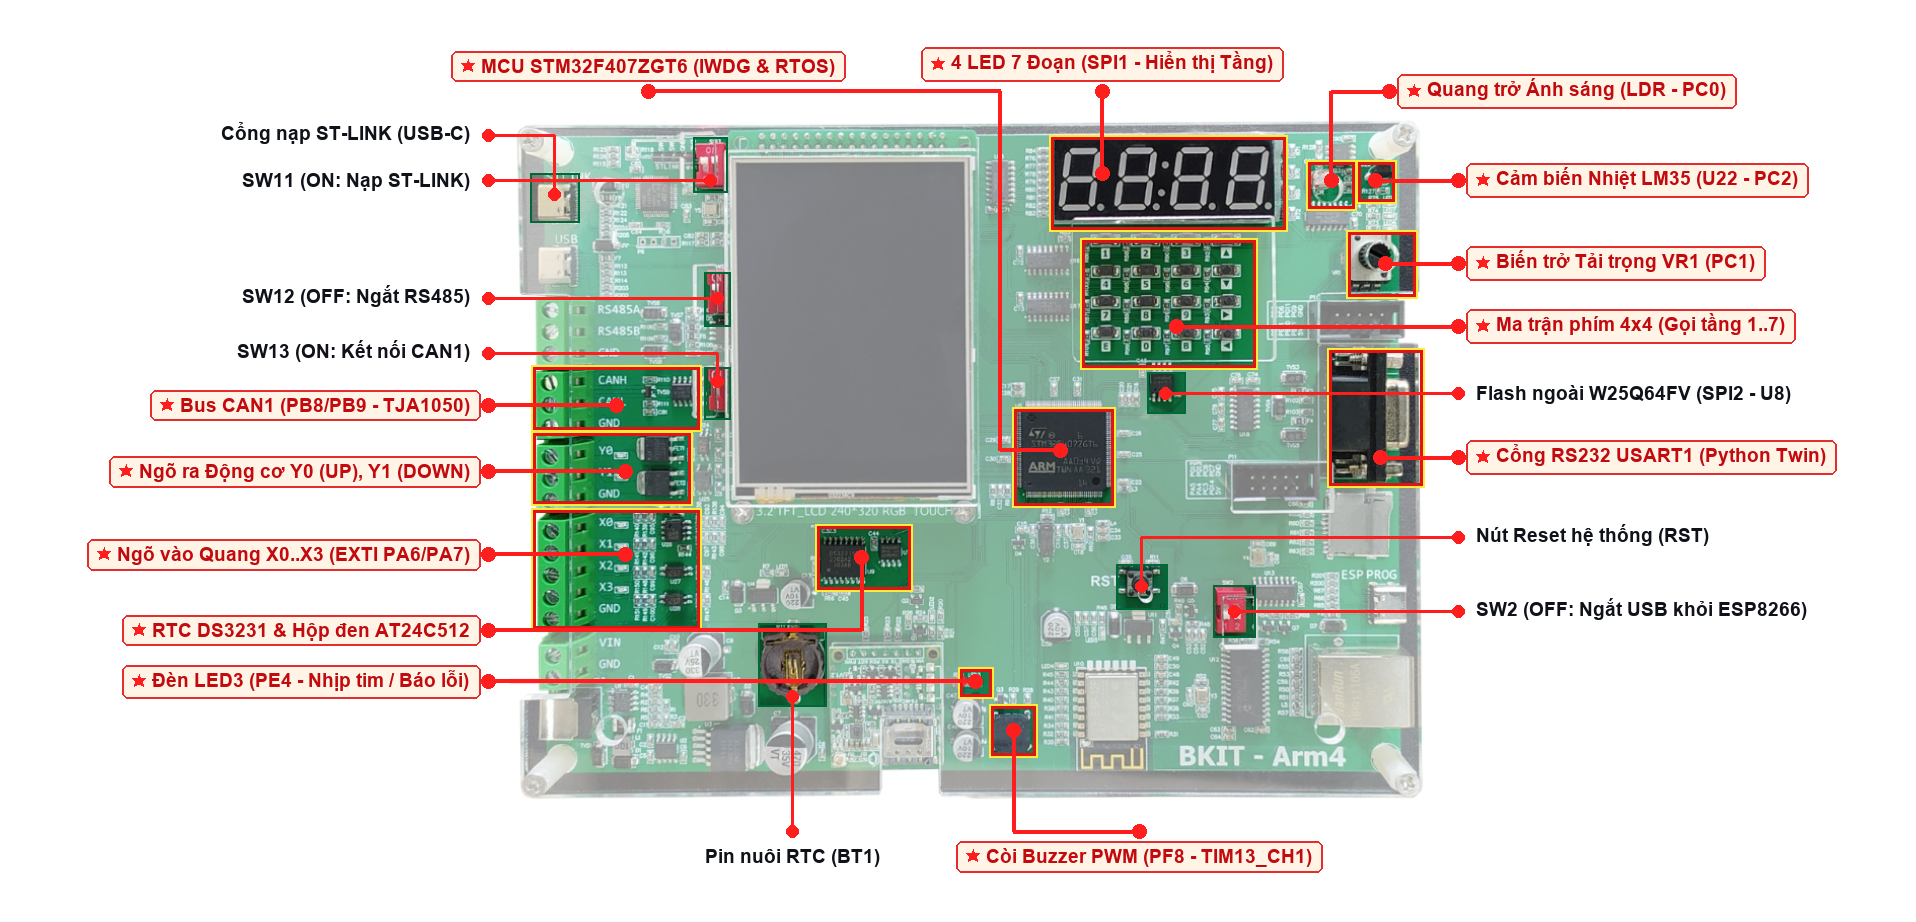
\includegraphics[width=\textwidth]{image/bkit_arm4_project_map.png}
\caption{Sơ đồ định vị thực tế 13 cụm ngoại vi cốt lõi và cấu hình DIP Switch trên bo mạch BKIT ARM4}
\label{fig:bkit_map}
\end{figure}

\newpage
\subsection{Phân tích Nguyên lý Giao tiếp 4 Phân hệ Ngoại vi trên Kit}
Nguyên lý kết nối phần cứng, mức điện áp và cơ chế phân xử bus của 4 phân hệ gồm:

\subsubsection{Phân hệ An toàn Cách ly Quang (\texttt{X0..X3}, \texttt{Y0..Y1}) và Còi xung \texttt{PWM PF8}}
\begin{itemize}[nosep]
    \item \textbf{Ngõ vào cách ly quang \texttt{Opto In X0..X3} (\texttt{PA6, PA7, PC4, PC5}):}
    \begin{itemize}[nosep]
        \item \textit{Cách ly và mức logic:} Tín hiệu công tắc và cảm biến đi qua tầng ghép quang \textit{optocoupler} giúp cách ly điện áp công nghiệp và chống nhiễu xung khỏi các chân vi điều khiển; ngõ vào cấu hình điện trở kéo lên nội và tích cực mức thấp, giữ mức cao ổn định khi hở mạch.
        \item \textit{Ngắt cứng \texttt{EXTI6/7} (\texttt{X0, X1}):} Hai chân \texttt{X0 (PA6 -- Kẹt cửa)} và \texttt{X1 (PA7 -- E-Stop)} cấu hình ngắt ngoài theo sườn tích cực, lập tức chụp giá trị bộ đếm chu kỳ phần cứng \texttt{DWT} trước khâu lọc rung tiếp điểm \texttt{40~ms} để định lượng độ trễ phần cứng ở mức micro-giây.
        \item \textit{Đọc định kỳ \texttt{X2/X3}:} Chân \texttt{X3 (PC5)} nối công tắc quá tải cơ khí được tác vụ giám sát an toàn lấy mẫu mỗi \texttt{100~ms} và hợp logic (OR) cùng ngưỡng cân \texttt{VR1} ($\ge 800\text{ kg}$), còn \texttt{X2 (PC4)} dự phòng cho cảm biến hành trình tầng.
    \end{itemize}
    \item \textbf{Ngõ ra cách ly quang \texttt{Y0/Y1} (\texttt{PE5/PE6}) và \texttt{LED3} (\texttt{PE4}):}
    \begin{itemize}[nosep]
        \item \textit{Điều khiển động cơ kéo:} Hai ngõ ra tích cực mức cao cách ly quang để kích rơ-le chiều \textbf{LÊN (\texttt{Y0 -- PE5})} và \textbf{XUỐNG (\texttt{Y1 -- PE6})}; mạch và logic điều khiển luôn áp dụng khóa liên động kép, tự động ngắt cả hai chân về mức \texttt{0} nếu xuất hiện lệnh xung đột.
        \item \textit{Đèn nhịp hệ thống (\texttt{PE4}):} \texttt{LED3} đóng vai đèn nhịp giám sát trực quan trạng thái vận hành, nháy chậm chu kỳ \texttt{800~ms} khi cabin làm việc bình thường và chuyển sang nháy nhanh \texttt{200~ms} ngay khi hệ thống phát sinh báo cháy hoặc sự cố an toàn.
    \end{itemize}
    \item \textbf{Còi cảnh báo \texttt{PWM PF8} (\texttt{TIM13\_CH1}):}
    \begin{itemize}[nosep]
        \item \textit{Cấu hình bộ định thời:} Chân \texttt{PF8} được ánh xạ sang chức năng thay thế \texttt{AF9} nối với \texttt{TIM13\_CH1}; xung nhịp timer trên bus \texttt{APB1} đạt \texttt{84~MHz}, qua bộ chia tần \texttt{/84} tạo chuẩn đếm \texttt{1~MHz} ($1~\mu\text{s/tick}$) để sinh dải tần chính xác.
        \item \textit{Phát âm không chặn:} Xuất xung vuông chu kỳ nhiệm vụ \texttt{50\%} giúp còi thụ động đạt âm lượng cực đại theo 5 âm báo chuẩn lưu trong Flash (\texttt{1.5..3.0~kHz}), có khóa \textit{mutex} đồng bộ truy cập và tự ngắt theo nhịp định thời không chặn trên tác vụ giao diện.
    \end{itemize}
\end{itemize}

\subsubsection{Phân hệ Đo lường Tương tự 5 Kênh (\texttt{ADC1 12-bit})}
Bộ chuyển đổi \texttt{ADC1} vận hành ở chế độ lấy mẫu đồng bộ, độ phân giải \texttt{12-bit} ($0..4095$) với điện áp tham chiếu nội ($V_{\text{REF}} = 3300\text{ mV}$, bước lượng tử $V_{\text{LSB}} \approx 0.806\text{ mV}$), độ lợi $1\times$ và bộ chia xung nhịp \texttt{/4}:
\begin{itemize}[nosep]
    \item \textbf{Cảm biến nhiệt độ \texttt{LM35} (\texttt{PC2 -- ADC1\_IN12}):} Tuân theo đặc tuyến tuyến tính chuẩn $10\text{ mV}/^\circ\text{C}$, được quy đổi trực tiếp từ điện áp \texttt{mV} sang đơn vị nguyên $0.1^\circ\text{C}$ ($1\text{ mV} \equiv 0.1^\circ\text{C}$, số học dấu phẩy tĩnh), tránh chi phí dấu phẩy động mà vẫn bảo đảm theo dõi chính xác ngưỡng cháy $55.0^\circ\text{C}/48.0^\circ\text{C}$.
    \item \textbf{Biến trở tải trọng \texttt{VR1} (\texttt{PC1 -- ADC1\_IN11}):} Quy đổi tuyến tính dải điện áp $0..3300\text{ mV}$ theo tỉ lệ $m_{\text{kg}} = (V_{\text{VR1}} / 3300) \times 1000\text{ kg}$ thành tải trọng giả lập $0..1000\text{ kg}$ thay thế \textit{loadcell}, kết hợp trễ hồi (\textit{hysteresis}) để chặn đóng cửa khi vượt ngưỡng $800\text{ kg}/750\text{ kg}$.
    \item \textbf{Ba kênh đo giám sát bổ trợ (\texttt{PC0, PB0, PB1}):} Thu nhận trực tiếp điện áp \texttt{mV} ($0..3300\text{ mV}$) từ quang trở \texttt{LDR (PC0 -- IN10)}, kênh đo áp nguồn bus (\texttt{PB0 -- IN8}) và dòng tải (\texttt{PB1 -- IN9}), phục vụ tự kiểm tra độ ổn định mạch tương tự và xuất thông số chẩn đoán qua giao diện dòng lệnh trên UART.
\end{itemize}

\subsubsection{Phân hệ Bus Dùng chung \texttt{SPI1}, \texttt{I2C1} và NOR Flash \texttt{SPI2}}
Đây là cụm ngoại vi chia sẻ bus vật lý, đòi hỏi đồng bộ chặt chẽ ở cả tầng phần cứng lẫn hệ điều hành thời gian thực (Hình~\ref{fig:shared_buses}):
\begin{itemize}[nosep]
    \item \textbf{Bus \texttt{SPI1} dùng chung (\texttt{PB3 SCK}, \texttt{PB4 MISO}, \texttt{PB5 MOSI}, \texttt{1~MHz}):}
    \begin{itemize}[nosep]
        \item \textit{Nhánh xuất LED 7 đoạn:} Sử dụng \textbf{2 $\times$ \texttt{74HC595}} mắc nối tiếp nhận \texttt{16-bit} dữ liệu (byte mã đoạn \texttt{a..g} và byte chọn vị trí LED) truyền bit có trọng số cao trước (\textit{MSB-first}), chốt đồng loạt bằng xung sườn lên \texttt{2~$\mu$s} trên chân \texttt{PG6 (LD\_LATCH)} ở tần số quét \texttt{100~Hz} để hiển thị tầng, mũi tên \texttt{UP/dn}, \texttt{FE} và \texttt{Err}.
        \item \textit{Nhánh nhập ma trận phím 4$\times$4:} Sử dụng \textbf{2 $\times$ \texttt{74HC165}} đọc 16 phím tích cực mức thấp; trước mỗi lượt quét chu kỳ \texttt{50~ms}, vi điều khiển phát xung nạp song song qua chân \texttt{PD3 (BTN\_LOAD)} rồi dịch 2 byte về \texttt{MISO (PB4)}, tự động lọc bỏ trạng thái nghỉ (\texttt{0xFFFF}) và nhiễu thả nổi (\texttt{0x0000}).
        \item \textit{Phân xử bus:} Do hai mạch thanh ghi dịch dùng chung đường xung nhịp \texttt{SCK (PB3)}, mọi giao dịch trên \texttt{SPI1} đều được tuần tự hóa bằng khóa \textit{mutex} phân xử bus có kế thừa độ ưu tiên (\textit{Priority Inheritance}), ngăn chặn hoàn toàn hiện tượng lem LED hay sai mã phím khi tác vụ quét đồng thời.
    \end{itemize}
    \item \textbf{Bus \texttt{I2C1} dùng chung (\texttt{PB6 SCL}, \texttt{PB7 SDA}, \textit{Fast-Mode} \texttt{400~kHz}):}
    \begin{itemize}[nosep]
        \item \textit{Đồng hồ \texttt{DS3231 RTC} (\texttt{0x68}):} Tích hợp pin dự phòng CR2032 giúp duy trì giờ chuẩn ngay cả khi mất nguồn chính; vi điều khiển đọc liên tiếp các thanh ghi \texttt{0x00..0x06} và giải mã từ dạng nhị phân thập phân (\texttt{BCD}) sang nhị phân thuần để gắn dấu thời gian cho từng bản ghi sự cố.
        \item \textit{Hộp đen \texttt{AT24C512 EEPROM} (\texttt{0x50}):} Dung lượng \texttt{64~KB} (\texttt{65\,536 Bytes}) tổ chức theo trang \texttt{128 Bytes}; vùng đầu (\texttt{0x0000}) lưu khối tiêu đề kiểm tra \texttt{CRC32}, còn vùng dữ liệu (\texttt{0x0080}) lưu bộ đệm vòng 32 bản ghi bước \texttt{32 Bytes} kèm \texttt{CRC16} nhằm bảo toàn nhật ký khi mất điện mà không ghi vượt ranh giới trang.
        \item \textit{Phân xử bus:} Hai thiết bị dùng chung đường truyền cực máng hở \texttt{PB6/PB7} nối điện trở kéo lên $R_{p1}, R_{p2}$ về nguồn \texttt{+3.3~V}, đồng thời mọi thao tác đọc/ghi thời gian hay hộp đen đều được tuần tự hóa qua khóa \textit{mutex} riêng của bus \texttt{I2C1} để tránh xung đột khung truyền.
    \end{itemize}
    \newpage
    \item \textbf{Bus \texttt{SPI2} độc lập (\texttt{PB12..PB15}, \texttt{2~MHz}):}
    \begin{itemize}[nosep]
        \item \textit{NOR Flash \texttt{W25Q64FV} (\texttt{8~MB}):} Vận hành trên bus \texttt{SPI2} tách biệt qua chân chọn chip \texttt{PB12} tích cực mức thấp nên không tranh chấp băng thông với nhánh HMI; khi khởi tạo hoặc kiểm tra phần cứng, firmware phát lệnh \texttt{0x9F} đọc về mã \texttt{JEDEC ID 0xEF 0x40 0x17} xác nhận kết nối.
    \end{itemize}
\end{itemize}

\begin{figure}[H]
\centering
\resizebox{\textwidth}{!}{%
\begin{tikzpicture}
    % ==================== NUA TRAI: SHARED SPI1 ====================
    \draw[draw=black!55, dashed, fill=black!2, line width=0.6pt] (-0.3, -4.55) rectangle (9.05, 3.65);
    \node[font=\footnotesize\bfseries, text=tablehead, anchor=west] at (-0.1, 3.30) {(a) Kiến trúc Bus \texttt{SPI1} Dùng chung (1 MHz)};

    % MCU SPI1 Master
    \node[acadmcu, text width=2.55cm, minimum height=4.8cm] (mcu_spi) at (1.30, -0.20)
        {\textbf{STM32F407}\\[-1pt]\texttt{SPI1 Master}\\[6pt]
         {\tiny Bộ phân xử:}\\[-1pt]
         {\tiny\textbf{Mutex Bus SPI1}}\\[-1pt]
         {\tiny (\textit{Priority Inheritance})}};

    % 2x 74HC595 + 4 LED 7 doan
    \node[acadbox, text width=3.10cm, minimum height=1.85cm] (hc595) at (7.20, 1.45)
        {\textbf{2 $\times$ IC \texttt{74HC595}}\\[-1pt]
         {\tiny Ghi dịch SIPO (16-bit)}\\[-1pt]
         {\tiny $\rightarrow$ \textbf{4 LED 7 đoạn Anode chung}}\\[-1pt]
         {\tiny Hiển thị \texttt{UP/dn}, \texttt{FE}, \texttt{Err} @ 100 Hz}};

    % 2x 74HC165 + Ma tran 16 phim
    \node[acadbox, text width=3.10cm, minimum height=1.85cm] (hc165) at (7.20, -1.95)
        {\textbf{2 $\times$ IC \texttt{74HC165}}\\[-1pt]
         {\tiny Ghi dịch PISO (16-bit)}\\[-1pt]
         {\tiny $\leftarrow$ \textbf{Ma trận 16 phím 4$\times$4}}\\[-1pt]
         {\tiny Active-Low (\texttt{0..15}, \texttt{0xFFFF}=idle)}};

    % Dau noi day bus SPI1 (kenh day rong ~2.7cm, nhan can giua khoang trong, tach hoan toan vien hop)
    \draw[acadarr] (mcu_spi.east |- 0, 1.95) -- node[acadpin, above=1.5pt, pos=0.44] {\texttt{PB3 (SCK)}} (hc595.west |- 0, 1.95);
    \draw[acadarr] (5.12, 1.95) |- ($(hc165.west)+(0, 0.50)$);
    \fill (5.12, 1.95) circle (1.4pt);

    \draw[acadarr] (mcu_spi.east |- 0, 1.25) -- node[acadpin, above=1.5pt, pos=0.44] {\texttt{PB5 (MOSI)}} (hc595.west |- 0, 1.25);
    \draw[acadarr] (hc165.west |- 0, -1.25) -- node[acadpin, above=1.5pt, pos=0.50] {\texttt{PB4 (MISO)}} (mcu_spi.east |- 0, -1.25);

    \draw[acadarr, draw=tablehead] (mcu_spi.east |- 0, 0.58) -- node[acadpin, above=1.5pt, pos=0.48] {\texttt{PG6 (LD\_LATCH)}} (hc595.west |- 0, 0.58);
    \draw[acadarr, draw=tablehead] (mcu_spi.east |- 0, -2.45) -- node[acadpin, above=1.5pt, pos=0.50] {\texttt{PD3 (BTN\_LOAD)}} (hc165.west |- 0, -2.45);

    \node[font=\tiny\itshape, align=center, text=black!80] at (4.35, -3.95)
        {Lưu ý: Tác vụ HMI khóa \textbf{Mutex Bus SPI1} trước khi tạo xung \texttt{PG6} hoặc \texttt{PD3},\\
         loại bỏ hoàn toàn nhiễu bấm phím làm nhòe LED 7 đoạn.};

    % ==================== NUA PHAI: SHARED I2C1 ====================
    \draw[draw=black!55, dashed, fill=black!2, line width=0.6pt] (9.35, -4.55) rectangle (19.15, 3.65);
    \node[font=\footnotesize\bfseries, text=tablehead, anchor=west] at (9.55, 3.30) {(b) Kiến trúc Bus \texttt{I2C1} Dùng chung (400 kHz)};

    % MCU I2C1 Master
    \node[acadmcu, text width=2.45cm, minimum height=4.2cm] (mcu_i2c) at (10.85, -0.35)
        {\textbf{STM32F407}\\[-1pt]\texttt{I2C1 Master}\\[6pt]
         {\tiny Bộ phân xử:}\\[-1pt]
         {\tiny\textbf{Mutex Bus I2C1}}\\[-1pt]
         {\tiny (\textit{Priority Inheritance})}};

    % Nguon 3.3V va dien tro keo len Rp (tach xa vien MCU va day doc bus I2C)
    \node[font=\tiny\bfseries] (vcc) at (14.40, 2.58) {\texttt{+3.3V}};
    \draw[acadline] (13.70, 2.33) -- (15.10, 2.33);
    % Rp1 SCL
    \draw[acadline] (14.00, 2.33) -- (14.00, 1.98);
    \draw[acadline, fill=white] (13.89, 1.43) rectangle (14.11, 1.98);
    \draw[acadline] (14.00, 1.43) -- (14.00, 0.85);
    \node[font=\tiny] at (13.60, 1.70) {$R_{p1}$};
    % Rp2 SDA
    \draw[acadline] (14.80, 2.33) -- (14.80, 1.98);
    \draw[acadline, fill=white] (14.69, 1.43) rectangle (14.91, 1.98);
    \draw[acadline] (14.80, 1.43) -- (14.80, 0.05);
    \node[font=\tiny] at (15.20, 1.70) {$R_{p2}$};

    % Duong bus SCL & SDA (nhan dat cach xa mep phai MCU >= 2.5mm)
    \draw[acadarr] (mcu_i2c.east |- 0, 0.85) -- (15.72, 0.85);
    \node[acadpin, anchor=south west] at (12.48, 0.90) {\texttt{PB6(SCL)}};
    \draw[acadbiarr] (mcu_i2c.east |- 0, 0.05) -- (15.72, 0.05);
    \node[acadpin, anchor=south west] at (12.48, 0.10) {\texttt{PB7(SDA)}};
    \fill (14.00, 0.85) circle (1.4pt);
    \fill (14.80, 0.05) circle (1.4pt);

    % 2 IC tren I2C1: DS3231 & AT24C512
    \node[acadbox, text width=2.85cm, minimum height=1.75cm] (ds3231) at (17.45, 1.45)
        {\textbf{IC \texttt{DS3231 RTC}}\\[-1pt]
         {\tiny Địa chỉ 7-bit: \texttt{0x68}}\\[-1pt]
         {\tiny Pin dự phòng CR2032}\\[-1pt]
         {\tiny Cung cấp giờ thực BCD}};

    \node[acadbox, text width=2.85cm, minimum height=1.95cm] (at24) at (17.45, -1.75)
        {\textbf{IC \texttt{AT24C512 EEPROM}}\\[-1pt]
         {\tiny Địa chỉ 7-bit: \texttt{0x50}}\\[-1pt]
         {\tiny 64 KB (Trang 128 B)}\\[-1pt]
         {\tiny Hộp đen 32 ô \texttt{CRC16/32}}};

    % Nhanh re xuong DS3231 & AT24C512 (o x=15.55 cach xa Rp2 o 15.20)
    \draw[acadline] (15.55, 0.85) |- ($(ds3231.west)+(0, 0.30)$);
    \draw[acadline] (15.55, 0.05) |- ($(ds3231.west)+(0, -0.30)$);
    \draw[acadline] (15.55, 0.85) |- ($(at24.west)+(0, 0.35)$);
    \draw[acadline] (15.55, 0.05) |- ($(at24.west)+(0, -0.25)$);
    \fill (15.55, 0.85) circle (1.4pt);
    \fill (15.55, 0.05) circle (1.4pt);

    \node[font=\tiny\itshape, align=center, text=black!80] at (14.25, -3.95)
        {Lưu ý: Loại bỏ \texttt{\&audio\_codec CS43L22} và chuyển \texttt{\&i2c1} về \texttt{PB6/PB7}\\
         giúp giải phóng hoàn toàn chân \texttt{PB9} cho bộ thu phát \texttt{CAN1\_TX}.};
\end{tikzpicture}%
}

\caption{Sơ đồ nguyên lý ghép nối và phân xử bus dùng chung \texttt{SPI1} (\texttt{74HC595} / \texttt{74HC165}) và \texttt{I2C1} (\texttt{DS3231} / \texttt{AT24C512})}
\label{fig:shared_buses}
\end{figure}

\subsubsection{Phân hệ Truyền thông Phân tán \texttt{CAN1} và Giao tiếp \texttt{USART1 RS232}}
\begin{itemize}[nosep]
    \item \textbf{Mạng \texttt{bxCAN1} tốc độ \texttt{500~kbps} (\texttt{PB8 CAN1\_RX}, \texttt{PB9 CAN1\_TX}):}
    \begin{itemize}[nosep]
        \item \textit{Giao tiếp vi sai chống nhiễu:} Bộ điều khiển \texttt{bxCAN1} chuẩn \texttt{CAN 2.0A} (ID 11-bit) xuất tín hiệu qua bộ thu phát vi sai \textbf{\texttt{TJA1050}} (đóng \texttt{SW13 = ON}) ra cặp dây \texttt{CANH / CANL} có trở đầu cuối \texttt{120~$\Omega$}, điểm lấy mẫu $87.5\%$ chu kỳ bit giúp miễn nhiễu công nghiệp.
        \item \textit{Chế độ vận hành linh hoạt:} Chuyển đổi linh hoạt giữa tự kiểm 1 kit (\texttt{LOOPBACK}) và nối mạng 2 kit (\texttt{NORMAL}: \texttt{CABIN} $\leftrightarrow$ \texttt{HALL}); bộ lọc phần cứng thu hẹp 3 dải ID trọng yếu (\texttt{0x080}, \texttt{0x100..0x10F}, \texttt{0x200..0x3FF}), hỗ trợ khung \texttt{RTR} và giám sát \texttt{TEC/REC} kèm cơ chế phục hồi lỗi bus.
    \end{itemize}
    \item \textbf{Cổng nối tiếp \texttt{USART1 RS232} (\texttt{PA9 TX}, \texttt{PA10 RX}, \texttt{115200 8N1}):}
    \begin{itemize}[nosep]
        \item \textit{Tầng chuyển mức:} Chuyển đổi mức áp \texttt{3.3~V TTL} sang chuẩn đối xứng RS232 qua IC \textbf{\texttt{MAX3232}} ra đầu DB9 về máy tính; gạt \texttt{SW12 = OFF} để cô lập hoàn toàn nhánh RS485 dùng chung chân truyền nhận.
        \item \textit{Kênh song công Shell \& Telemetry:} Đảm nhiệm đồng thời giao diện dòng lệnh \textbf{Zephyr Shell CLI} phục vụ chẩn đoán ngoại vi và luồng bản tin JSON \texttt{\$TWIN} mỗi \texttt{200~ms} đồng bộ trạng thái thời gian thực lên \textbf{PC Digital Twin}.
    \end{itemize}
\end{itemize}

\clearpage
\subsection{Thiết kế Devicetree (\texttt{app.overlay}) và Giải quyết Xung đột Chân}
Bo mạch \textbf{BKIT ARM4} dùng vi điều khiển \texttt{STM32F407ZGT6} (vỏ \texttt{LQFP144}), trong khi bo chuẩn gần nhất của Zephyr RTOS là \texttt{stm32f4\_disco} (\texttt{STM32F407VGT6}, vỏ \texttt{LQFP100}). Do khác biệt số chân I/O và ngoại vi hàn sẵn trên bo Discovery (âm thanh \texttt{cs43l22@4a}, \texttt{usbotg\_fs}, \texttt{leds}, \texttt{gpio\_keys}), việc giữ nguyên cây thiết bị gốc sẽ gây xung đột chân. Tệp phủ \texttt{app.overlay} được viết để chuyển hướng \texttt{chosen} (\texttt{\&usart1}, \texttt{\&can1}), chuẩn hóa \texttt{aliases} (\texttt{led0..2}, \texttt{sw0..3}, \texttt{watchdog0}, \texttt{eeprom-0}, \texttt{pwm-buzzer}) và xử lý 3 nhóm xung đột chính (Hình~\ref{fig:dt_conflict}):
\begin{enumerate}[nosep]
    \item \textbf{Tách chân \texttt{PA6} khỏi \texttt{\&adc1} để dành cho ngắt cứng \texttt{X0}:}
    \begin{itemize}[nosep]
        \item \textit{Xung đột gốc:} Trên \texttt{stm32f4\_disco}, \texttt{pinctrl-0} mặc định của \texttt{\&adc1} ánh xạ cả \texttt{adc1\_in6\_pa6}, trong khi kit \textbf{BKIT ARM4} nối \texttt{PA6} với ngõ vào quang \texttt{X0} đòi hỏi ngắt sườn phát hiện kẹt cửa tức thời.
        \item \textit{Can thiệp \texttt{app.overlay}:} Ghi đè \texttt{pinctrl-0} của \texttt{\&adc1} chỉ giữ 5 kênh (\texttt{PB0, PB1, PC0, PC1, PC2}), khai báo 5 nút \texttt{channel@8..c} (\texttt{12-bit}, \texttt{ADC\_REF\_INTERNAL}, \texttt{SYNC}), tắt \texttt{gpio\_keys} mặc định và gán \texttt{PA6} cho \texttt{bkit\_in\_x0} (\texttt{sw0}).
        \item \textit{Kết quả:} Giải phóng hoàn toàn \texttt{PA6} làm ngắt sườn \texttt{EXTI6} cho cảm biến kẹt cửa \texttt{X0}, tách bạch khỏi chu kỳ quét 5 kênh của \texttt{ADC1}.
    \end{itemize}
    \item \textbf{Tách \texttt{\&i2c1} khỏi chân \texttt{PB9} để giải phóng \texttt{CAN1\_TX}:}
    \begin{itemize}[nosep]
        \item \textit{Xung đột gốc:} Mặc định \texttt{\&i2c1} dùng chân \texttt{i2c1\_sda\_pb9} cho codec âm thanh \texttt{cs43l22@4a}, trùng trực tiếp với chân phát \texttt{CAN1\_TX (PB9)} nối IC \texttt{TJA1050}, đồng thời tồn tại nhiều nút ngoại vi dư thừa dễ tranh chấp chân.
        \item \textit{Can thiệp \texttt{app.overlay}:} Chuyển \texttt{\&i2c1} dùng \texttt{I2C\_BITRATE\_FAST} (\texttt{400~kHz}) tại cặp \texttt{PB6 (SCL) / PB7 (SDA)}, khai báo \texttt{eeprom@50} (\texttt{atmel,at24}, \texttt{64~KB}, trang \texttt{128~B}), tắt các nút \texttt{\&audio\_codec}, \texttt{\&can2}, \texttt{\&usart2}, \texttt{\&i2s3}, \texttt{\&usbotg\_fs}, \texttt{\&timers2/4}, \texttt{leds}, \texttt{pwmleds}; và gán \texttt{\&can1} ra \texttt{PB8/PB9} (\texttt{500~kbps}, \texttt{sample-point = <875>}).
        \item \textit{Kết quả:} Bus vi sai \texttt{bxCAN1} (\texttt{PB8/PB9}) và \texttt{I2C1} (\texttt{PB6/PB7}) phục vụ \texttt{DS3231 RTC} cùng \texttt{AT24C512} vận hành song song không đụng chân.
    \end{itemize}
    \item \textbf{Kích hoạt \texttt{GPIOF/G}, nút \texttt{zephyr,user} và bổ sung \texttt{pinctrl} cho \texttt{PF8}:}
    \begin{itemize}[nosep]
        \item \textit{Giới hạn gốc:} Vỏ \texttt{LQFP100} không khai báo Port F và Port G nên cây thiết bị gốc thiếu định tuyến chân còi \texttt{PF8 (TIM13\_CH1)} và chốt LED 7 đoạn \texttt{PG6 (LD\_LATCH)}.
        \item \textit{Can thiệp \texttt{app.overlay}:} Bật tường minh \texttt{\&gpiof}, \texttt{\&gpiog}, \texttt{\&timers13} (\texttt{st,prescaler = <83>}) và \texttt{\&iwdg}; tạo mới \texttt{tim13\_ch1\_pf8} (\texttt{STM32\_PINMUX('F', 8, AF9)}) cho \texttt{bkit\_buzzer}; đồng thời gom 5 \texttt{io-channels} và 3 chân điều khiển (\texttt{ld-latch-gpios = <\&gpiog 6>}, \texttt{btn-load-gpios = <\&gpiod 3>}, \texttt{w25q-cs-gpios = <\&gpiob 12>}) vào \texttt{zephyr,user}.
        \item \textit{Kết quả:} Khai thác trọn vẹn tài nguyên \texttt{LQFP144} gồm còi \texttt{PWM13 (PF8)}, chốt \texttt{74HC595 (PG6)}, nạp phím \texttt{74HC165 (PD3)} và chọn NOR Flash \texttt{PB12}.
    \end{itemize}
\end{enumerate}

\clearpage
\begin{figure}[H]
\centering
\resizebox{\textwidth}{!}{%
\begin{tikzpicture}
    % Tieu de 3 cot (khop rong voi 3 cot ben duoi, khong bao gio de nhau)
    \node[acadhdr, text width=4.65cm, minimum height=0.68cm] (H1) at (2.5, 4.75)  {TARGET \texttt{stm32f4\_disco} (\texttt{LQFP100})};
    \node[acadhdr, text width=4.85cm, minimum height=0.68cm, fill=tablehead, text=white] (H2) at (8.05, 4.75)  {CAN THIỆP TRONG \texttt{app.overlay}};
    \node[acadhdr, text width=4.85cm, minimum height=0.68cm] (H3) at (13.6, 4.75) {ÁNH XẠ \texttt{BKIT ARM4} (\texttt{LQFP144})};

    % Hang 1: Xung dot PA6
    \node[acadbox, text width=4.65cm, minimum height=1.55cm] (C1L) at (2.5, 3.25)
        {\textbf{Xung đột 1: Chân \texttt{PA6}}\\[1pt]
         {\tiny Mặc định \texttt{\&adc1} gán \texttt{adc1\_in6\_pa6}}\\
         {\tiny $\Rightarrow$ Chiếm dụng chân ngắt cứng \texttt{X0}}};

    \node[acadboxnav, text width=4.85cm, minimum height=1.55cm] (C1M) at (8.05, 3.25)
        {\texttt{\&adc1} ghi đè \texttt{pinctrl-0}:\\[1pt]
         {\tiny Chỉ giữ 5 kênh \texttt{PB0, PB1, PC0, PC1, PC2}}\\
         {\tiny Khai báo \texttt{bkit\_in\_x0: PA6 (ACTIVE\_LOW)}}};

    \node[acadbox, text width=4.85cm, minimum height=1.55cm] (C1R) at (13.6, 3.25)
        {\textbf{\texttt{PA6} $\rightarrow$ Ngắt cứng \texttt{EXTI6} (\texttt{X0})}\\[1pt]
         {\tiny Phát hiện vật cản cửa cabin (tức thời)}\\
         {\tiny Tách bạch hoàn toàn với 5 kênh \texttt{ADC1}}};

    % Hang 2: Xung dot PB9
    \node[acadbox, text width=4.65cm, minimum height=1.55cm] (C2L) at (2.5, 1.30)
        {\textbf{Xung đột 2: Chân \texttt{PB9}}\\[1pt]
         {\tiny Mặc định \texttt{\&i2c1} dùng \texttt{i2c1\_sda\_pb9}}\\
         {\tiny nối codec \texttt{cs43l22@4a} $\Rightarrow$ Đụng \texttt{CAN1\_TX}}};

    \node[acadboxnav, text width=4.85cm, minimum height=1.55cm] (C2M) at (8.05, 1.30)
        {\texttt{\&i2c1} chuyển \texttt{PB6/PB7} (\texttt{400 kHz}):\\[1pt]
         {\tiny Gắn \texttt{status = "disabled"} cho \texttt{\&audio\_codec},}\\
         {\tiny \texttt{\&can2}, \texttt{\&usart2}, \texttt{\&i2s3}, \texttt{\&timers2/4}}};

    \node[acadbox, text width=4.85cm, minimum height=1.55cm] (C2R) at (13.6, 1.30)
        {\textbf{\texttt{PB8/PB9} $\rightarrow$ \texttt{CAN1} | \texttt{PB6/7} $\rightarrow$ \texttt{I2C1}}\\[1pt]
         {\tiny \texttt{bxCAN1} 500 kbps (\texttt{TJA1050}) \& \texttt{DS3231/}}\\
         {\tiny \texttt{AT24C512} chạy đồng thời không xung đột}};

    % Hang 3: Port F va Port G thieu tren LQFP100
    \node[acadbox, text width=4.65cm, minimum height=1.55cm] (C3L) at (2.5, -0.65)
        {\textbf{Xung đột 3: Thiếu Port \texttt{F/G}}\\[1pt]
         {\tiny Vỏ \texttt{LQFP100} không có cổng \texttt{GPIOF/G}}\\
         {\tiny $\Rightarrow$ Không có nút còi \texttt{PF8} \& chốt \texttt{PG6}}};

    \node[acadboxnav, text width=4.85cm, minimum height=1.55cm] (C3M) at (8.05, -0.65)
        {Bật \texttt{\&gpiof}, \texttt{\&gpiog}, \texttt{\&timers13}:\\[1pt]
         {\tiny Khai báo mới \texttt{tim13\_ch1\_pf8 (AF9)}}\\
         {\tiny Gán \texttt{ld-latch-gpios = <\&gpiog 6>}}};

    \node[acadbox, text width=4.85cm, minimum height=1.55cm] (C3R) at (13.6, -0.65)
        {\textbf{\texttt{PF8} $\rightarrow$ \texttt{PWM13} | \texttt{PG6} $\rightarrow$ \texttt{LD\_LATCH}}\\[1pt]
         {\tiny Còi xung PWM đa âm báo (\texttt{TIM13\_CH1})}\\
         {\tiny Chốt dữ liệu 4 LED 7 đoạn qua \texttt{74HC595}}};

    % Mui ten ket noi giua 3 cot
    \foreach \r in {1, 2, 3} {
        \draw[acadarr] (C\r L.east) -- (C\r M.west);
        \draw[acadarr] (C\r M.east) -- (C\r R.west);
    }
\end{tikzpicture}%
}

\caption{Kiến trúc ánh xạ Devicetree giải quyết 3 xung đột phần cứng từ \texttt{stm32f4\_disco} (\texttt{LQFP100}) sang BKIT ARM4 (\texttt{LQFP144})}
\label{fig:dt_conflict}
\end{figure}

Đoạn trích cấu hình từ \texttt{app.overlay} dưới đây minh họa trực tiếp cách phân giải xung đột \texttt{pinctrl} và khai báo thiết bị \texttt{AT24C512} / \texttt{bxCAN1}:

\begin{lstlisting}[language=C, caption={Trích đoạn cấu hình giải quyết xung đột chân và bus ngoại vi trong app.overlay}]
&gpiof { status = "okay"; };  &gpiog { status = "okay"; };
&pinctrl {
    tim13_ch1_pf8: tim13_ch1_pf8 { pinmux = <STM32_PINMUX('F',8,AF9)>; };
};
/* Go bo adc1_in6_pa6 de giai phong PA6 cho ngat cung EXTI6 (X0) */
&adc1 {
    pinctrl-0 = <&adc1_in8_pb0 &adc1_in9_pb1
                 &adc1_in10_pc0 &adc1_in11_pc1 &adc1_in12_pc2>;
    pinctrl-names = "default"; status = "okay";
};
&audio_codec { status = "disabled"; };
/* Chuyen I2C1 ve PB6/PB7 de tranh xung dot PB9 voi CAN1_TX */
&i2c1 {
    pinctrl-0 = <&i2c1_scl_pb6 &i2c1_sda_pb7>;
    clock-frequency = <I2C_BITRATE_FAST>; status = "okay";
    at24_eeprom: eeprom@50 {
        compatible = "atmel,at24"; reg = <0x50>;
        size = <65536>; pagesize = <128>;
    };
};
/* CAN1 500 kbps qua TJA1050 (yeu cau SW13 = ON) */
&can1 {
    pinctrl-0 = <&can1_rx_pb8 &can1_tx_pb9>;
    bitrate = <500000>; sample-point = <875>; status = "okay";
};
\end{lstlisting}

\clearpage
\subsection{Cấu hình Công tắc DIP Switch và Bảng Ánh xạ Chân Tổng hợp}
Trước khi cấp nguồn và nạp firmware xuống kit \textbf{BKIT ARM4}, 4 công tắc gạt DIP Switch cần được đặt đúng vị trí quy định ở Bảng~\ref{tab:switches} để đấu nối chính xác mạch nạp và bộ thu phát \texttt{CAN}. Bảng~\ref{tab:pinmap} tổng hợp toàn bộ ánh xạ chân \texttt{STM32F407ZGT6} và driver Zephyr tương ứng.

\begingroup
\renewcommand{\arraystretch}{1.14}%
\setlength{\tabcolsep}{4.5pt}%
\fontsize{8.3}{10.4}\selectfont
\arrayrulecolor{tableborder}%
\begin{xltabular}{\textwidth}{|C{2.0cm}|C{2.0cm}|Y|}
\caption{Cấu hình 4 cụm công tắc DIP Switch bắt buộc trên bo mạch BKIT ARM4}\label{tab:switches}\\
\hline
\rowcolor{tablehead}
\thcell{Công tắc} & \thcell{Trạng thái} & \thcell{Tác dụng phần cứng trên bo mạch BKIT ARM4} \\
\hline
\endfirsthead
\hline
\rowcolor{tablehead}
\thcell{Công tắc} & \thcell{Trạng thái} & \thcell{Tác dụng phần cứng trên bo mạch BKIT ARM4} \\
\hline
\endhead
\hline
\endfoot
\hline
\endlastfoot
\texttt{SW11} & \textbf{ON} & Kết nối mạch nạp/gỡ lỗi tích hợp \textbf{ST-LINK} với chân \texttt{SWDIO/SWCLK} của \texttt{STM32F407}. \\
\hline
\rowcolor{roweven}
\texttt{SW13} & \textbf{ON} & Nối cặp chân \texttt{PB8 (CAN1\_RX) / PB9 (CAN1\_TX)} vào IC thu phát vi sai \textbf{TJA1050}. \\
\hline
\texttt{SW12} & \textbf{OFF} & Cách ly khối thu phát RS485 để tránh xung đột tải trên đường truyền nối tiếp. \\
\hline
\rowcolor{roweven}
\texttt{SW2} & \textbf{OFF} & Ngắt kết nối UART từ cổng USB-C sang module ESP8266 khi làm việc trực tiếp với STM32. \\
\end{xltabular}
\endgroup

\begingroup
\renewcommand{\arraystretch}{1.12}%
\setlength{\tabcolsep}{4.5pt}%
\fontsize{8.1}{10.1}\selectfont
\arrayrulecolor{tableborder}%
\begin{xltabular}{\textwidth}{|L{2.6cm}|L{2.8cm}|L{3.0cm}|Y|}
\caption{Bảng ánh xạ chân vi điều khiển STM32F407ZGT6 và Driver Zephyr trong \texttt{app.overlay}}\label{tab:pinmap}\\
\hline
\rowcolor{tablehead}
\thcell{Ngoại vi / Bus} & \thcell{Chân MCU} & \thcell{Driver / Alias} & \thcell{Vai trò trong Hệ thống Thang máy} \\
\hline
\endfirsthead
\hline
\rowcolor{tablehead}
\thcell{Ngoại vi / Bus} & \thcell{Chân MCU} & \thcell{Driver / Alias} & \thcell{Vai trò trong Hệ thống Thang máy} \\
\hline
\endhead
\hline
\endfoot
\hline
\endlastfoot
\texttt{LED3 Debug} & \texttt{PE4} & \texttt{gpio-leds} (\texttt{led0}) & Nháy Heartbeat RTOS (chậm bình thường, chớp nhanh khi lỗi). \\
\hline
\rowcolor{roweven}
\texttt{Opto Out Y0/Y1} & \texttt{PE5 / PE6} & \texttt{gpio-leds} (\texttt{led1/2}) & Rơ-le quang điều khiển động cơ \textbf{CHẠY LÊN (Y0)} / \textbf{CHẠY XUỐNG (Y1)}. \\
\hline
\texttt{Opto In X0..X3} & \texttt{PA6, PA7, PC4, PC5} & \texttt{gpio-keys} (\texttt{sw0..sw3}) & \texttt{X0}: Chống kẹt cửa (EXTI6); \texttt{X1}: E-Stop (EXTI7); \texttt{X2}: Tầng; \texttt{X3}: Quá tải. \\
\hline
\rowcolor{roweven}
\texttt{Buzzer PWM} & \texttt{PF8} (\texttt{TIM13\_CH1}) & \texttt{pwm-leds} (\texttt{AF9}) & Phát âm báo đa tần số \texttt{1.5..3.0 kHz} không chặn (\textit{non-blocking}). \\
\hline
\texttt{ADC1 Sensors} & \texttt{PC2, PC1, PC0} & \texttt{adc\_dt} (\texttt{IN12,11,10}) & \texttt{PC2}: Nhiệt độ LM35 ($10~\text{mV}/^\circ\text{C}$); \texttt{PC1}: Biến trở tải \texttt{VR1}; \texttt{PC0}: Quang trở. \\
\hline
\rowcolor{roweven}
\texttt{ADC1 Power} & \texttt{PB0, PB1} & \texttt{adc\_dt} (\texttt{IN8, IN9}) & Giám sát điện áp đường nguồn (\texttt{PB0}) và dòng tải tiêu thụ (\texttt{PB1}). \\
\hline
\texttt{Shared SPI1} & \texttt{PB3/4/5 + PG6/PD3} & \texttt{spi\_stm32} (Mutex bus) & Quét 4 LED 7 đoạn (\texttt{2$\times$74HC595}, \texttt{PG6}) và 16 phím 4$\times$4 (\texttt{2$\times$74HC165}, \texttt{PD3}). \\
\hline
\rowcolor{roweven}
\texttt{Shared I2C1} & \texttt{PB6 / PB7} & \texttt{i2c\_stm32} (Mutex bus) & Đọc đồng hồ thực \texttt{DS3231} (\texttt{0x68}) và ghi hộp đen \texttt{AT24C512} (\texttt{0x50}). \\
\hline
\texttt{SPI2 Flash} & \texttt{PB12..PB15} & \texttt{spi\_stm32} (\texttt{w25q-cs}) & Kiểm tra nhận dạng chip NOR Flash \texttt{W25Q64FV} (JEDEC ID \texttt{0xEF 0x40 0x17}). \\
\hline
\rowcolor{roweven}
\texttt{CAN1 Bus} & \texttt{PB8 / PB9} & \texttt{st,stm32-bxcan} & Mạng CAN 500 kbps (\texttt{TJA1050}), hỗ trợ \texttt{LOOPBACK} 1 kit và \texttt{NORMAL} 2 kit. \\
\hline
\texttt{USART1 RS232} & \texttt{PA9 / PA10} & \texttt{uart\_stm32} (115200) & Giao diện dòng lệnh Zephyr Shell CLI \& luồng telemetry \texttt{\$TWIN} lên PC. \\
\hline
\end{xltabular}
\endgroup

\clearpage
\section{THIẾT KẾ VÀ HIỆN THỰC FIRMWARE}

\subsection{Tổ chức Mã nguồn theo Kiến trúc Phân lớp Mô-đun}
Để tách biệt rõ ràng giữa thuật toán điều khiển và thao tác thanh ghi phần cứng, 13 tệp mã nguồn C trong thư mục \texttt{smart\_elevator\_zephyr/} được phân chia thành 4 tầng chức năng độc lập, thuận tiện cho bảo trì và kiểm thử từng phân hệ trên Zephyr Shell (Bảng~\ref{tab:modules}):
\begin{itemize}[nosep]
    \item \textbf{Tầng Hỗ trợ Bo mạch (\texttt{src/bsp/}):} Đóng gói toàn bộ thao tác thanh ghi và driver thiết bị Zephyr của 6 nhóm ngoại vi vật lý trên bo mạch BKIT ARM4; cung cấp các hàm API an toàn luồng (\textit{thread-safe}) lên tầng trên.
    \item \textbf{Tầng Logic Cốt lõi (\texttt{src/core/}):} Chứa Máy trạng thái phân cấp 9 trạng thái (\texttt{elevator\_hsm.c}) và bộ lập lịch hai chiều \texttt{SCAN/LOOK} (\texttt{elevator\_scheduler.c}), được thiết kế hoàn toàn độc lập với phần cứng để kiểm chứng logic xác định (\textit{deterministic}).
    \item \textbf{Tầng Truyền thông Phân tán (\texttt{src/comms/}):} Đảm nhiệm giao thức mạng \texttt{CAN1 500 kbps} (\texttt{can\_bus.c}) và đóng gói luồng dữ liệu JSON \texttt{\$TWIN} (\texttt{twin\_telemetry.c}) gửi lên máy tính.
    \item \textbf{Tầng Giao diện Dòng lệnh (\texttt{src/cli/}):} Cung cấp hai bộ lệnh Shell tương tác qua cổng \texttt{USART1 RS232} gồm \texttt{elev *} (vận hành \& tiêm lỗi HIL) và \texttt{bkit *} (chẩn đoán phần cứng). Mỗi mô-đun đăng ký một định danh \texttt{LOG\_MODULE\_REGISTER} riêng để kỹ sư bật/tắt log từng phân hệ ngay khi hệ thống đang chạy.
\end{itemize}

\begingroup
\renewcommand{\arraystretch}{1.20}%
\setlength{\tabcolsep}{4.5pt}%
\fontsize{8.2}{10.5}\selectfont
\arrayrulecolor{tableborder}%
\begin{xltabular}{\textwidth}{|L{2.2cm}|L{3.3cm}|Y|C{1.8cm}|}
\caption{Cấu trúc phân lớp 13 mô-đun mã nguồn C và định danh gỡ lỗi (\texttt{LOG\_MODULE\_\allowbreak REGISTER})}\label{tab:modules}\\
\hline
\rowcolor{tablehead}
\thcell{Phân lớp} & \thcell{Tệp mã nguồn (.c)} & \thcell{Chức năng kỹ thuật chính} & \thcell{Log Tag} \\
\hline
\endfirsthead
\hline
\rowcolor{tablehead}
\thcell{Phân lớp} & \thcell{Tệp mã nguồn (.c)} & \thcell{Chức năng kỹ thuật chính} & \thcell{Log Tag} \\
\hline
\endhead
\hline
\endfoot
\hline
\endlastfoot
\textbf{Ứng dụng} & \texttt{src/main.c} & Khởi tạo hệ thống, 5 \texttt{k\_timer} ISR \& 7 luồng RTOS tĩnh hướng sự kiện. & \texttt{app\_main} \\
\hline
\rowcolor{roweven}
\textbf{BSP Layer} & \texttt{bsp\_gpio\_exti.c} & Điều khiển \texttt{PE4..PE6}, khóa liên động motor, ngắt EXTI \texttt{X0/X1} (\texttt{DWT}). & \texttt{bsp\_gpio} \\
\hline
\textbf{BSP Layer} & \texttt{bsp\_pwm\_buzzer.c} & Còi PWM \texttt{PF8} (\texttt{TIM13\_CH1}), bảng tra mẫu âm Flash + \texttt{k\_mutex}. & \texttt{bsp\_pwm} \\
\hline
\rowcolor{roweven}
\textbf{BSP Layer} & \texttt{bsp\_adc\_sensors.c} & Đọc ADC1 5 kênh (\texttt{PC2 LM35}, tải \texttt{VR1}, quang trở, áp, dòng). & \texttt{bsp\_adc} \\
\hline
\textbf{BSP Layer} & \texttt{bsp\_spi\_hmi.c} & Shared \texttt{SPI1} (4 LED 7 đoạn \texttt{PG6}, 16 phím \texttt{PD3}) \& \texttt{SPI2 W25Q64}. & \texttt{bsp\_spi} \\
\hline
\rowcolor{roweven}
\textbf{BSP Layer} & \texttt{bsp\_i2c\_storage.c} & Shared \texttt{I2C1}: đồng hồ \texttt{DS3231} \& hộp đen \texttt{AT24C512} (\texttt{CRC16/32}). & \texttt{bsp\_i2c} \\
\hline
\textbf{BSP Layer} & \texttt{bsp\_watchdog.c} & \texttt{IWDG} 2500~ms, đọc nguyên nhân reset \texttt{HWINFO}, giám sát đa luồng. & \texttt{bsp\_wdt} \\
\hline
\rowcolor{roweven}
\textbf{Core Layer} & \texttt{elevator\_scheduler.c} & Bộ lập lịch hai chiều SCAN/LOOK dùng mặt nạ bit 7 tầng $O(1)$. & \texttt{elev\_sched} \\
\hline
\textbf{Core Layer} & \texttt{elevator\_hsm.c} & HSM 9 trạng thái, chu kỳ 100~ms, bộ đếm \texttt{atomic\_t} \& ma trận V-Model. & \texttt{elev\_hsm} \\
\hline
\rowcolor{roweven}
\textbf{Comms Layer} & \texttt{can\_bus.c} & CAN1 500~kbps (\texttt{tx\_cb}, \texttt{RTR}), 3 HW filter, role \texttt{CABIN/HALL}, Fail-Safe. & \texttt{can\_bus} \\
\hline
\textbf{Comms Layer} & \texttt{twin\_telemetry.c} & Đóng gói và truyền khung JSON \texttt{\$TWIN} chu kỳ 200~ms qua \texttt{USART1}. & \texttt{twin\_tx} \\
\hline
\rowcolor{roweven}
\textbf{CLI Layer} & \texttt{cli\_elev.c} & Lệnh \texttt{elev}: \texttt{status}, \texttt{call}, \texttt{door}, \texttt{fault}, \texttt{role}, \texttt{coverage}, \texttt{log}. & \texttt{cli\_elev} \\
\hline
\textbf{CLI Layer} & \texttt{cli\_bkit\_test.c} & Lệnh \texttt{bkit}: chẩn đoán ngoại vi (\texttt{adc}, \texttt{io}, \texttt{7seg}, \texttt{key}, \texttt{rtc}, \texttt{canping}). & \texttt{cli\_bkit} \\
\end{xltabular}
\endgroup

\subsection{Kiến trúc 7 Luồng RTOS Tĩnh Hướng Sự kiện và Đồng bộ hóa}
Để xử lý đồng thời các tín hiệu an toàn thời gian thực mà không tranh chấp CPU hay phân mảnh RAM, phần mềm trên nhân \textbf{Zephyr RTOS v4.4.0} được tổ chức thành 7 luồng liên kết chặt chẽ theo chuỗi \textit{Ngữ cảnh ngắt (ISR) $\rightarrow$ Đồng bộ Kernel $\rightarrow$ Luồng xử lý $\rightarrow$ Bảo vệ tài nguyên} (Hình~\ref{fig:rtos_arch} và Bảng~\ref{tab:threads}), tuân thủ 4 nguyên tắc cốt lõi:
\begin{itemize}[nosep]
    \item \textbf{Khởi tạo tĩnh toàn bộ \& Vận hành phi thăm dò (\textit{Static Allocation \& Zero-Polling}):}
    \begin{itemize}[nosep]
        \item Cả 7 luồng (\texttt{t1\_safety}..\texttt{t5\_wdt}) cùng toàn bộ đối tượng đồng bộ (\texttt{k\_sem}, \texttt{k\_msgq}, \texttt{k\_mutex}, \texttt{k\_timer}) đều được cấp phát tĩnh lúc biên dịch bằng \texttt{K\_THREAD\_DEFINE}, loại bỏ hoàn toàn cấp phát động (\texttt{malloc/heap}) và nguy cơ phân mảnh RAM.
        \item Mỗi luồng được ấn định độ trễ khởi chạy \texttt{500~ms} để hàm \texttt{main()} hoàn tất khởi tạo ngoại vi và ghi bản ghi bật nguồn vào hộp đen trước khi tác vụ vận hành; khi rảnh, luồng ngủ hoàn toàn trên \texttt{k\_sem\_take} hoặc \texttt{k\_msgq\_get} với cờ \texttt{K\_FOREVER}, chỉ thức dậy khi có ngắt hoặc nhịp định thời.
    \end{itemize}
    \item \textbf{Kỷ luật ngắt tối giản không chặn (\textit{Non-Blocking Minimal ISR}):}
    \begin{itemize}[nosep]
        \item Trong ngữ cảnh ngắt ngoài (\texttt{exti\_x0\_handler}, \texttt{exti\_x1\_handler}), 5 bộ định thời \texttt{K\_TIMER\_DEFINE} (\texttt{g\_safety\_timer}, \texttt{g\_hsm\_tick\_timer}, \texttt{g\_can\_hb\_timer}, \texttt{g\_hmi\_timer}, \texttt{g\_wdt\_timer}) và callback phát CAN (\texttt{can\_tx\_done\_cb}), mã ngắt chỉ thực hiện ba việc tức thời: chụp bộ đếm chu kỳ phần cứng \texttt{k\_cycle\_get\_32()} trước khâu lọc rung \texttt{40~ms}, tăng biến nguyên tử \texttt{atomic\_t} và đánh thức luồng qua \texttt{k\_sem\_give()} hoặc \texttt{k\_msgq\_put(..., K\_NO\_WAIT)}.
        \item Tuyệt đối cấm gọi \texttt{LOG\_*} đồng bộ, khóa \texttt{k\_mutex} hay giao tiếp \texttt{SPI/I2C} bên trong ISR; cấu hình \texttt{CONFIG\_LOG\_MODE\_DEFERRED} đẩy việc in log về tác vụ nền để giữ thời gian chiếm dụng ngắt ngắn nhất.
    \end{itemize}
    \item \textbf{Phân cấp ưu tiên tiền chiếm theo thời hạn (\textit{Deadline-Monotonic Priority 2..8}):}
    \begin{itemize}[nosep]
        \item Độ ưu tiên phản ánh trực tiếp thời hạn đáp ứng: \texttt{t1\_safety} (mức \textbf{2}) đáp ứng tức thời ngắt \texttt{X0/X1} và lấy mẫu 5 kênh \texttt{ADC1} (\texttt{100~ms}); \texttt{t2\_fsm} (mức \textbf{3}) điều hành HSM 9 trạng thái; cụm 3 luồng \texttt{t3\_can\_rx/tx/wdt} (mức \textbf{4}) tách rời thu/phát/giám sát mất kết nối \texttt{2000~ms} tránh chặn chéo; \texttt{t4\_hmi} (mức \textbf{5}) quét 4 LED 7 đoạn (\texttt{100~Hz}), 16 phím (\texttt{50~ms}), còi \texttt{PF8} và đèn \texttt{PE4}.
        \item Riêng \texttt{t5\_wdt} giữ mức ưu tiên thấp nhất (\textbf{8}) để quét check-in 4 luồng giám sát (\texttt{t1\_safety}, \texttt{t2\_fsm}, \texttt{t3\_can\_tx}, \texttt{t4\_hmi}) qua khóa spinlock nhẹ \texttt{g\_wdt\_lock} (ngưỡng treo \texttt{1500~ms}) trước khi nạp \texttt{IWDG} (\texttt{2500~ms}), đồng thời xuất JSON \texttt{\$TWIN} mỗi \texttt{200~ms} mà không làm trễ luồng an toàn.
    \end{itemize}
    \item \textbf{Đồng bộ đa lớp \& Chống đảo ngược độ ưu tiên (\textit{Priority Inheritance}):}
    \begin{itemize}[nosep]
        \item \textit{Trên bus vật lý dùng chung:} \texttt{g\_spi1\_bus\_mutex} tuần tự hóa giao dịch \texttt{SPI1} (LED \texttt{74HC595} và phím \texttt{74HC165}), còn \texttt{g\_i2c1\_bus\_mutex} bảo vệ cặp thiết bị \texttt{DS3231}/\texttt{AT24C512} trên \texttt{I2C1} giữa \texttt{t2\_fsm} (mức 3), \texttt{t3\_can\_tx} (mức 4) cùng giao diện \texttt{Shell CLI}.
        \item \textit{Trên dữ liệu trạng thái chia sẻ:} \texttt{g\_hsm\_state\_mutex}, \texttt{g\_can\_state\_mutex} và \texttt{g\_buzzer\_mutex} bảo đảm nhất quán ảnh chụp giữa luồng điều khiển ưu tiên cao với tác vụ xuất telemetry \texttt{t5\_wdt} (mức 8). Nhờ cơ chế \textit{Priority Inheritance} của \texttt{k\_mutex}, nhân Zephyr tự nâng tạm độ ưu tiên của luồng giữ khóa lên ngang mức luồng chờ ưu tiên cao để hoàn tất giao dịch và nhả khóa ngay lập tức.
    \end{itemize}
\end{itemize}

\begin{figure}[H]
\centering
\resizebox{\textwidth}{!}{%
\begin{tikzpicture}
    % Tieu de 4 cot (khoang ho giua cac cot >= 1.25cm -> tuyet doi khong chong day/mui ten)
    \node[acadhdr, text width=3.80cm, minimum height=0.72cm] at (2.05, 8.30) {1. NGỮ CẢNH NGẮT\\{\tiny (Non-Blocking ISR)}};
    \node[acadhdr, text width=3.20cm, minimum height=0.72cm] at (7.05, 8.30) {2. ĐỒNG BỘ KERNEL\\{\tiny (\texttt{k\_sem} / \texttt{k\_msgq})}};
    \node[acadhdr, text width=5.00cm, minimum height=0.72cm, fill=tablehead, text=white] at (12.85, 8.30) {3. 7 LUỒNG RTOS TĨNH\\{\tiny (\texttt{K\_THREAD\_DEFINE})}};
    \node[acadhdr, text width=3.75cm, minimum height=0.72cm] at (18.85, 8.30) {4. KHÓA \texttt{MUTEX} \& I/O\\{\tiny (\textit{Priority Inheritance})}};

    % Cot 1: Nguon danh thuc ISR (x=2.05, east ~ 4.13)
    \node[acadbox, text width=3.80cm, minimum height=1.35cm] (I1) at (2.05, 6.95)
        {\textbf{Ngắt cứng \texttt{EXTI6 / EXTI7}}\\[1pt]
         {\tiny \texttt{X0(PA6)}, \texttt{X1(PA7)} (lọc rung 40ms)}\\
         {\tiny Chụp \texttt{k\_cycle\_get\_32()} (\texttt{DWT})}};

    \node[acadbox, text width=3.80cm, minimum height=1.40cm] (I2) at (2.05, 4.70)
        {\textbf{5 Bộ định thời \texttt{k\_timer}}\\[1pt]
         {\tiny \texttt{safety}(100ms) $\cdot$ \texttt{hsm}(100ms)}\\
         {\tiny \texttt{can\_hb}(250ms) $\cdot$ \texttt{hmi}(10ms) $\cdot$ \texttt{wdt}}};

    \node[acadbox, text width=3.80cm, minimum height=1.35cm] (I3) at (2.05, 2.55)
        {\textbf{Ngắt bộ điều khiển \texttt{bxCAN1}}\\[1pt]
         {\tiny 3 HW Filter (\texttt{0x080, 0x10x, 0x200+})}\\
         {\tiny \texttt{can\_tx\_done\_cb} $\rightarrow$ \texttt{atomic\_t}}};

    \node[acadbox, text width=3.80cm, minimum height=1.35cm] (I4) at (2.05, 0.50)
        {\textbf{Zephyr Shell CLI / HIL}\\[1pt]
         {\tiny \texttt{USART1 (115200)}: \texttt{elev call/fault}}\\
         {\tiny Phím ma trận 4$\times$4 (\texttt{0..15})}};

    % Cot 2: Kernel Sync Primitives (x=7.05, west ~ 5.27, east ~ 8.83)
    \node[acadbox, text width=3.20cm, minimum height=1.10cm] (K1) at (7.05, 6.95)
        {\texttt{g\_safety\_wakeup\_sem}\\[1pt]{\tiny \texttt{k\_sem} (Đánh thức T1)}};

    \node[acadboxnav, text width=3.20cm, minimum height=1.35cm] (K2) at (7.05, 4.70)
        {\texttt{g\_hsm\_event\_msgq}\\[1pt]
         {\tiny \texttt{k\_msgq} (32 gói sự kiện)}\\
         {\tiny Hội tụ Phần cứng thật \& HIL}};

    \node[acadbox, text width=3.20cm, minimum height=1.35cm] (K3) at (7.05, 2.55)
        {\texttt{g\_can\_rx\_msgq} \&\\[-1pt]
         \texttt{g\_can\_partner\_sem}\\[1pt]
         {\tiny Timeout \texttt{2000 ms} (-EAGAIN)}};

    \node[acadbox, text width=3.20cm, minimum height=1.20cm] (K4) at (7.05, 0.50)
        {\texttt{g\_hmi\_sem} (10ms) \&\\[-1pt]
         \texttt{g\_wdt\_sem} (100ms)};

    % Cot 3: 7 Luong RTOS (x=12.85, west ~ 10.17, east ~ 15.53)
    \node[acadbox, text width=5.00cm, minimum height=0.86cm] (T1) at (12.85, 6.95)
        {\textbf{\texttt{t1\_safety}} {\tiny [Prio 2 -- 1536 B]}\\[-1pt]
         {\tiny Đọc \texttt{ADC1} (5 ch) + Hysteresis \texttt{LM35/VR1}}};
    \node[acadbox, text width=5.00cm, minimum height=0.86cm] (T2) at (12.85, 5.77)
        {\textbf{\texttt{t2\_fsm}} {\tiny [Prio 3 -- 2048 B]}\\[-1pt]
         {\tiny HSM 9 trạng thái + \texttt{SCAN/LOOK} + Khóa L1}};
    \node[acadbox, text width=5.00cm, minimum height=0.86cm] (T3a) at (12.85, 4.59)
        {\textbf{\texttt{t3\_can\_rx}} {\tiny [Prio 4 -- 1536 B]}\\[-1pt]
         {\tiny Giải mã CAN, trả lời \texttt{RTR}, cấp \texttt{partner\_sem}}};
    \node[acadbox, text width=5.00cm, minimum height=0.86cm] (T3b) at (12.85, 3.41)
        {\textbf{\texttt{t3\_can\_tx}} {\tiny [Prio 4 -- 1536 B]}\\[-1pt]
         {\tiny Phát HB/Status 250ms, phục hồi \texttt{BUS-OFF}}};
    \node[acadbox, text width=5.00cm, minimum height=0.86cm] (T3c) at (12.85, 2.23)
        {\textbf{\texttt{t3\_can\_wdt}} {\tiny [Prio 4 -- 1024 B]}\\[-1pt]
         {\tiny Giám sát \texttt{partner\_sem} 2000ms $\rightarrow$ \texttt{FAIL\_SAFE}}};
    \node[acadbox, text width=5.00cm, minimum height=0.86cm] (T4) at (12.85, 1.05)
        {\textbf{\texttt{t4\_hmi}} {\tiny [Prio 5 -- 1536 B]}\\[-1pt]
         {\tiny Quét 7Seg (\texttt{PG6}), 16 phím (\texttt{PD3}), Còi \texttt{PF8}}};
    \node[acadbox, text width=5.00cm, minimum height=0.86cm] (T5) at (12.85, -0.13)
        {\textbf{\texttt{t5\_wdt}} {\tiny [Prio 8 -- 1536 B]}\\[-1pt]
         {\tiny Kiểm tra check-in \texttt{IWDG} \& Xuất JSON \texttt{\$TWIN}}};

    % Cot 4: 4 Khoi Tai nguyen xep DUNG THU TU TUONG UNG T1..T5 -> KHONG BAO GIO CAT CHEO!
    % (x=18.85, west ~ 16.79)
    \node[acadboxnav, text width=3.75cm, minimum height=1.38cm] (R1) at (18.85, 6.45)
        {\textbf{Khóa Liên động Lớp 2}\\[1pt]
         {\tiny \texttt{bsp\_gpio\_set\_motor\_outputs()}}\\
         {\tiny Cấm \texttt{PE5} \& \texttt{PE6} bật đồng thời}};

    \node[acadboxnav, text width=3.75cm, minimum height=1.38cm] (R2) at (18.85, 4.15)
        {\textbf{\texttt{g\_i2c1\_bus\_mutex}}\\[1pt]
         {\tiny (\textit{Priority Inheritance})}\\
         {\tiny \texttt{DS3231} (\texttt{0x68}) + \texttt{AT24C512} (\texttt{0x50})}};

    \node[acadboxnav, text width=3.75cm, minimum height=1.42cm] (R3) at (18.85, 1.75)
        {\textbf{\texttt{g\_spi1\_bus\_mutex}}\\[1pt]
         {\tiny (\textit{Priority Inheritance})}\\
         {\tiny 2$\times$\texttt{74HC595} (\texttt{PG6}) \& 2$\times$\texttt{74HC165} (\texttt{PD3})}};

    \node[acadboxnav, text width=3.75cm, minimum height=1.18cm] (R4) at (18.85, -0.25)
        {\textbf{Hardware \texttt{IWDG} (2500 ms)}\\[1pt]
         {\tiny Chỉ nạp \texttt{wdt\_feed()} khi đủ 4 check-in}};

    % === KENH 1 -> 2 (x = 4.13 .. 5.27 -> cac track 4.52 va 4.88 cach deu, thoang) ===
    \draw[acadarr] (I1.east) -- (K1.west);
    \draw[acadarr] (I2.east) -- (K2.west);
    \draw[acadarr] ($(I2.east)+(0,-0.32)$) -- (4.88, 4.38) |- (K4.west |- 0, 0.72);
    \draw[acadarr] (I3.east) -- (K3.west);
    \draw[acadarr] (I4.east) -- (4.52, 0.50) |- (K2.west |- 0, 4.30);

    % === KENH 2 -> 3 (x = 8.83 .. 10.17 -> tach rieng tung duong theo y, khong dinh chum) ===
    \draw[acadarr] (K1.east) -- (T1.west);
    \draw[acadarr] (K2.east) -- (9.35, 4.70) |- (T2.west);
    \draw[acadarr] ($(K3.east)+(0, 0.25)$) -- (9.65, 2.80) |- (T3a.west);
    \draw[acadarr] ($(K3.east)+(0,-0.25)$) -- (9.65, 2.30) |- (T3c.west);
    \draw[acadarr] ($(K4.east)+(0, 0.22)$) -- (9.35, 0.72) |- (T4.west);
    \draw[acadarr] ($(K4.east)+(0,-0.22)$) -- (9.35, 0.28) |- (T5.west);

    % Duong Post Event tu T1 quay lai K2 (chay o y=6.24 -> sach phia tren T2=5.77 & duoi K1=6.40)
    \draw[acaddash] ($(T1.west)+(0,-0.22)$) -- (9.85, 6.73) |- (7.05, 6.24) -- (K2.north);

    % === KENH 3 -> 4 (x = 15.53 .. 16.79 -> 100% PHANG, 0 DUONG CAT NHAU!) ===
    \draw[acadarr] (T1.east) -- (16.15, 6.95) |- ($(R1.west)+(0, 0.28)$);
    \draw[acadarr] ($(T2.east)+(0, 0.16)$) -- (15.90, 5.93) |- ($(R1.west)+(0,-0.25)$);
    \draw[acadarr] ($(T2.east)+(0,-0.20)$) -- (16.35, 5.57) |- ($(R2.west)+(0, 0.25)$);
    \draw[acadarr] (T3b.east) -- (16.10, 3.41) |- ($(R2.west)+(0,-0.25)$);
    \draw[acadarr] (T4.east) -- (16.15, 1.05) |- (R3.west);
    \draw[acadarr] (T5.east) -- (16.15, -0.13) |- (R4.west);
\end{tikzpicture}%
}

\caption{Kiến trúc 7 luồng RTOS tĩnh hướng sự kiện, ngắt cứng (ISR), hàng đợi \texttt{k\_msgq} và đồng bộ hóa \texttt{k\_mutex}}
\label{fig:rtos_arch}
\end{figure}

\begingroup
\renewcommand{\arraystretch}{1.20}%
\setlength{\tabcolsep}{4.5pt}%
\fontsize{8.1}{10.4}\selectfont
\arrayrulecolor{tableborder}%
\begin{xltabular}{\textwidth}{|L{2.1cm}|C{1.4cm}|C{1.4cm}|Y|L{3.7cm}|}
\caption{Đặc tả 7 luồng thời gian thực tĩnh hướng sự kiện trong \texttt{src/main.c}}\label{tab:threads}\\
\hline
\rowcolor{tablehead}
\thcell{Tên Thread} & \thcell{Ưu tiên} & \thcell{Stack} & \thcell{Nhiệm vụ kỹ thuật chính} & \thcell{Đối tượng đồng bộ / ISR} \\
\hline
\endfirsthead
\hline
\rowcolor{tablehead}
\thcell{Tên Thread} & \thcell{Ưu tiên} & \thcell{Stack} & \thcell{Nhiệm vụ kỹ thuật chính} & \thcell{Đối tượng đồng bộ / ISR} \\
\hline
\endhead
\hline
\endfoot
\hline
\endlastfoot
\texttt{t1\_safety} & 2 (Cao) & 1536~B & Đáp ứng ngắt EXTI \texttt{X0/X1}; đọc ADC1 5 kênh kèm lọc Hysteresis (\texttt{LM35}, \texttt{VR1}). & \texttt{g\_safety\_wakeup\_sem},\newline\texttt{g\_safety\_timer} (100~ms) \\
\hline
\rowcolor{roweven}
\texttt{t2\_fsm} & 3 & 2048~B & Thực thi HSM 9 trạng thái, khóa liên động \texttt{PE5/PE6} và lập lịch SCAN/LOOK. & \texttt{g\_hsm\_event\_msgq},\newline\texttt{g\_hsm\_tick\_timer} (100~ms) \\
\hline
\texttt{t3\_can\_rx} & 4 & 1536~B & Nhận khung CAN1 (\texttt{K\_FOREVER}), phân tách \texttt{RTR}/Data, cấp \texttt{partner\_sem}. & \texttt{g\_can\_rx\_msgq},\newline\texttt{g\_can\_partner\_sem} \\
\hline
\rowcolor{roweven}
\texttt{t3\_can\_tx} & 4 & 1536~B & Phát trạng thái/Heartbeat 250~ms, giám sát \texttt{TEC/REC} \& phục hồi \texttt{can\_recover()}. & \texttt{g\_can\_hb\_sem},\newline\texttt{g\_can\_hb\_timer} (250~ms) \\
\hline
\texttt{t3\_can\_wdt} & 4 & 1024~B & Chờ \texttt{partner\_sem} ngưỡng 2000~ms; kích Fail-Safe ngay khi gặp \texttt{-EAGAIN}. & \texttt{k\_sem\_take(..., 2000~ms)},\newline\texttt{k\_sem\_reset()} \\
\hline
\rowcolor{roweven}
\texttt{t4\_hmi} & 5 & 1536~B & Quét 4 LED 7 đoạn (\texttt{PG6}), 16 phím 4$\times$4 (\texttt{PD3}), còi \texttt{PF8} \& đèn \texttt{PE4}. & \texttt{g\_hmi\_timer} (10~ms),\newline\texttt{g\_spi1\_bus\_mutex} \\
\hline
\texttt{t5\_wdt} & 8 (Thấp) & 1536~B & Kiểm tra 4 check-in (\texttt{bsp\_wdt\_service()}) 100~ms và xuất \texttt{\$TWIN} mỗi 200~ms. & \texttt{g\_wdt\_timer} (100~ms),\newline\texttt{g\_wdt\_lock}, \texttt{g\_hsm\_state\_mutex} \\
\end{xltabular}
\endgroup

\subsection{Máy Trạng thái Phân cấp 9 Trạng thái (HSM), Khóa Liên động Kép và Hội tụ Sự kiện}
Để đồng bộ hành vi cabin giữa thực tế với kiểm thử và ngăn bật nhầm hai chiều động cơ, lõi điều khiển (Hình~\ref{fig:hsm_states} và Bảng~\ref{tab:hsm_table}) chạy theo nhịp \texttt{100~ms} (\texttt{EV\_TICK\_100MS}) với 3 cơ chế:
\begin{itemize}[nosep]
    \item \textbf{Phân cấp 9 Trạng thái (HSM) và Luồng Chuyển tiếp (Hình~\ref{fig:hsm_states}):}
    \begin{itemize}[nosep]
        \item \textit{Chu trình Bình thường (\texttt{Superstate}, \texttt{1..7}):} Từ \texttt{INIT} tại Tầng 1, thang về \texttt{IDLE\_CLOSED} để bộ lập lịch \texttt{LOOK} chọn hướng: mở cửa tại chỗ nếu gọi cùng tầng, hoặc chạy \texttt{MOVING\_UP/DOWN} (\texttt{1500~ms/tầng}) tới khi \texttt{elev\_sched\_should\_stop()} thỏa. Chu trình cửa chạy qua \texttt{DOOR\_OPENING} (\texttt{700~ms}), \texttt{DOOR\_OPEN} (giữ \texttt{1800~ms}, treo mở nếu quá tải $\ge 800\text{ kg}$) và \texttt{DOOR\_CLOSING} (\texttt{700~ms}); nếu kẹt cửa \texttt{X0} khi đang đóng, HSM giữ nguyên \texttt{resume\_pct} để mở ngược lại ngay.
        \item \textit{Tiền chiếm Khẩn cấp (\texttt{8..9}, ngoài \texttt{Superstate}):} Ngắt ngang mọi trạng thái thường không cần lặp cung: \textbf{\texttt{FIRE\_EVAC}} (khi \texttt{LM35} $\ge 55^\circ\text{C}$, Phím \texttt{10} hoặc \texttt{CAN 0x080}) xóa hàng đợi, đóng cửa (nếu tầng $>1$), chạy về Tầng 1 mở cửa thoát và về \texttt{IDLE\_CLOSED} khi $\le 48^\circ\text{C}$ \& hết lỗi; \textbf{\texttt{FAIL\_SAFE}} (\texttt{E-Stop X1} hoặc đứt CAN $>2000\text{ ms}$) cắt ngay \texttt{Y0/Y1=0}, mở cửa nếu mất CAN rồi đóng lại khi nối mạng, hoặc khóa chờ \texttt{EV\_CLEAR\_FAULT}.
        \item \textit{Đo Độ phủ V-Model (\texttt{hsm\_transition}):} Mọi chuyển tiếp hợp lệ tăng cạnh \texttt{transition\_matrix[9][9]} và bật \texttt{visited\_states\_mask} cho lệnh \texttt{elev coverage}.
    \end{itemize}
    \item \textbf{Khóa Liên động Động cơ 2 Tầng Độc lập (\textit{Dual-Layer Motor Interlock}):}
    \begin{itemize}[nosep]
        \item \textit{Lớp 1 -- Core (\texttt{drive\_interlocked\_outputs} / \texttt{elevator\_hsm.c}):} Chỉ bật \texttt{Y0} (\texttt{MOVING\_UP}) hoặc \texttt{Y1} (\texttt{MOVING\_DOWN}, hay hạ tầng \texttt{FIRE\_EVAC} từ tầng $>1$) khi \texttt{door\_pos == DOOR\_POS\_CLOSED} và \texttt{!estop\_active}.
        \item \textit{Lớp 2 -- BSP (\texttt{bsp\_gpio\_set\_motor\_outputs} / \texttt{bsp\_gpio\_exti.c}):} Kiểm tra chéo \texttt{up\_en} và \texttt{down\_en} trước khi ghi GPIO; nếu cùng bằng \texttt{true}, lập tức cắt \texttt{PE5=0, PE6=0}, ghi log lỗi và trả \texttt{-EINVAL}.
    \end{itemize}
    \item \textbf{Cơ chế Hội tụ Hai Nhánh Sự kiện (Phần cứng thật \& Tiêm lỗi HIL/CLI):}
    \begin{itemize}[nosep]
        \item Qua \texttt{elevator\_hsm\_post\_event()} (Hình~\ref{fig:event_convergence}), các gói sự kiện \texttt{elevator\_event\_t} hội tụ về \texttt{g\_hsm\_event\_msgq} từ \textbf{Nhánh Phần cứng thật} (\texttt{LM35}, \texttt{VR1}, \texttt{X0/X1}, phím \texttt{4$\times$4 PD3}) và \textbf{Nhánh HIL/CLI} (nút \textit{Inject} trên \textbf{PC Digital Twin}, lệnh \texttt{elev fault/call}, \texttt{CAN 0x080/0x10x}).
        \item Hàm \texttt{elevator\_hsm\_step()} rút tuần tự từng gói cập nhật \texttt{g\_hsm}, bảo đảm HIL và vận hành thật dùng chung mã rơ-le \texttt{PE5/PE6}, còi \texttt{PF8}, LED 7 đoạn và \texttt{AT24C512}.
    \end{itemize}
\end{itemize}

\begin{figure}[H]
\centering
\resizebox{\textwidth}{!}{%
\begin{tikzpicture}[
    umlstate/.style={
        rectangle split, rectangle split parts=2,
        rectangle split part align={center, left},
        draw=black!85, fill=white, line width=0.8pt,
        rounded corners=3pt, font=\scriptsize, inner sep=3.5pt,
        rectangle split part fill={black!4, white}
    },
    umlemerg/.style={
        rectangle split, rectangle split parts=2,
        rectangle split part align={center, left},
        draw=tablehead, fill=white, line width=1.05pt,
        rounded corners=3pt, font=\scriptsize, inner sep=4pt,
        rectangle split part fill={tablehead!12, white}
    }
]
    % === SUPERSTATE: NORMAL OPERATION ===
    \draw[draw=black!70, dashed, line width=0.75pt, rounded corners=4pt, fill=black!1]
        (-0.4, -4.55) rectangle (16.6, 5.15);
    \node[font=\scriptsize\bfseries, text=tablehead, anchor=west] at (-0.2, 4.82)
        {SUPERSTATE: VẬN HÀNH BÌNH THƯỜNG \quad {\tiny\normalfont\itshape(Khóa liên động: \texttt{Y0/Y1 = 1} $\iff$ \texttt{door\_pos == CLOSED \&\& !estop})}};

    % Initial pseudostate [*]
    \fill[black!90] (0.0, 2.75) circle (3.2pt);

    % Hang tren: INIT, IDLE_CLOSED, MOVING_UP, MOVING_DOWN
    \node[umlstate, text width=2.25cm] (S_INIT) at (1.65, 2.75) {
        \textbf{1. INIT}
        \nodepart{second}
        \tiny \texttt{floor = 1}\\
        \tiny \texttt{door = CLOSED (0\%)}\\
        \tiny \texttt{Y0 = 0, Y1 = 0}
    };

    \node[umlstate, text width=3.20cm, draw=tablehead, line width=1.0pt] (S_IDLE) at (5.55, 2.75) {
        \textbf{2. IDLE\_CLOSED}
        \nodepart{second}
        \tiny \texttt{entry / Y0=0, Y1=0, dir=IDLE}\\
        \tiny \texttt{LED 7Seg: F- [floor]}\\
        \tiny \texttt{do / elev\_sched\_pick\_next()}
    };

    \node[umlstate, text width=2.95cm] (S_UP) at (10.35, 2.75) {
        \textbf{6. MOVING\_UP}
        \nodepart{second}
        \tiny \texttt{entry / Y0(PE5)=1, Y1=0}\\
        \tiny \texttt{LED 7Seg: UP [\_/-/¯] [f]}\\
        \tiny \texttt{do / +1 tầng mỗi 1500 ms}
    };

    \node[umlstate, text width=3.55cm] (S_DN) at (14.65, 2.75) {
        {\scriptsize\textbf{7. MOVING\_DOWN}}
        \nodepart{second}
        \tiny \texttt{entry / Y0=0, Y1(PE6)=1}\\
        \tiny \texttt{LED 7Seg: dn [¯/-/\_] [f]}\\
        \tiny \texttt{do / -1 tầng mỗi 1500 ms}
    };

    % Hang duoi trong Superstate: Chu trinh cua
    \node[umlstate, text width=3.55cm] (S_OPENING) at (2.15, -1.85) {
        \textbf{3. DOOR\_OPENING}
        \nodepart{second}
        \tiny \texttt{entry / Y0=0, Y1=0, Còi arrived}\\
        \tiny \texttt{do / door\_pct: 0 -> 100\% (700 ms)}
    };

    \node[umlstate, text width=3.85cm] (S_OPEN) at (7.90, -1.85) {
        \textbf{4. DOOR\_OPEN}
        \nodepart{second}
        \tiny \texttt{entry / Đếm giữ cửa 1800 ms}\\
        \tiny \texttt{do / Giữ mở nếu \texttt{overload >= 800kg}}\\
        \tiny \texttt{     hoặc \texttt{fire \&\& floor == 1}}
    };

    \node[umlstate, text width=3.55cm] (S_CLOSING) at (13.85, -1.85) {
        \textbf{5. DOOR\_CLOSING}
        \nodepart{second}
        \tiny \texttt{do / door\_pct: 100 -> 0\% (700 ms)}\\
        \tiny \texttt{guard / Theo dõi \texttt{EXTI6 X0} (\texttt{PA6})}
    };

    % === 2 TRANG THAI KHAN CAP (UU TIEN TOI CAO) ===
    \node[umlemerg, text width=7.1cm] (S_FIRE) at (3.65, -6.50) {
        \textbf{8. FIRE\_EVAC (Sơ tán Hỏa hoạn Khẩn cấp)}
        \nodepart{second}
        \tiny \texttt{trigger / LM35 >= 55.0°C} | Phím \texttt{10} | CAN \texttt{0x080}\\
        \tiny \texttt{do / Xóa hàng đợi, đóng cửa, chạy thẳng Tầng 1 \& Mở cửa}\\
        \tiny \texttt{LED: FE [f] | Thoát khi \texttt{EV\_CLEAR} \&\& LM35 <= 48.0°C}
    };

    \node[umlemerg, text width=7.3cm] (S_FAIL) at (12.35, -6.50) {
        \textbf{9. FAIL\_SAFE (Khóa An toàn / Dừng Khẩn cấp)}
        \nodepart{second}
        \tiny \texttt{trigger / E-Stop X1 (PA7)} | Phím \texttt{11} | Đứt CAN \texttt{> 2000 ms}\\
        \tiny \texttt{entry / Cắt ngay \texttt{Y0=0, Y1=0}; mở cửa nếu lỗi CAN}\\
        \tiny \texttt{LED: Err [f] | Phục hồi khi \texttt{EV\_FAULT\_CLEAR} (Phím \texttt{12..15})}
    };

    % === CHUYEN TIEP HANG TREN ===
    \draw[acadarr] (0.12, 2.75) -- (S_INIT.west);
    \draw[acadarr] (S_INIT.east) -- node[acadlbl, above=2pt] {\tiny Boot OK} (S_IDLE.west);
    \draw[acadarr] (S_IDLE.east) -- node[acadlbl, above=2pt] {\tiny\texttt{target>cur}} (S_UP.west);
    \draw[acadarr] ($(S_IDLE.north)+(0.4,0)$) -- ++(0, 0.55) -| node[acadlbl, pos=0.25] {\tiny\texttt{target < cur} (Chạy xuống)} ($(S_DN.north)+(-0.2,0)$);

    % === CHUYEN TIEP DI XUONG & QUAY VE (CAC DUONG CACH NHAU 0.55CM, KHONG CAT CHONG) ===
    \draw[acadarr] (S_IDLE.south -| S_OPENING.north) -- node[acadlbl, pos=0.45] {\tiny\texttt{target == cur}} (S_OPENING.north);
    \draw[acadarr] (S_UP.south) -- ++(0, -0.52) -| node[acadlbl, pos=0.25] {\tiny Chạm tầng cần dừng (\texttt{LOOK})} ($(S_OPENING.north)+(0.95,0)$);
    \draw[acadarr] (S_DN.south) -- ++(0, -1.08) -| node[acadlbl, pos=0.18] {\tiny Chạm tầng đích} ($(S_OPENING.north)+(1.45,0)$);

    \draw[acadarr] ($(S_CLOSING.north)+(-0.85,0)$) -- ++(0, 0.88) -| node[acadlbl, pos=0.25] {\tiny Đóng kín \texttt{0\%} (\texttt{700 ms})} ($(S_IDLE.south)+(0.85,0)$);

    % === CHUYEN TIEP GIUA 3 TRANG THAI CUA ===
    \draw[acadarr] (S_OPENING.east) -- node[acadlbl, above=2pt] {\tiny \texttt{700ms (100\%)}} (S_OPEN.west);
    \draw[acadarr] (S_OPEN.east) -- node[acadlbl, above=2pt] {\tiny \texttt{1800ms \& <=750kg}} (S_CLOSING.west);

    % === CUNG PHAN XA CHONG KET CUA X0 ===
    \draw[acadarr, line width=0.9pt] ($(S_CLOSING.south)+(0,-0.02)$) -- ++(0, -0.82) -|
        node[acadlbl, pos=0.25] {\textbf{Kẹt cửa \texttt{X0 (PA6)} / Phím \texttt{9} / Quá tải $\ge 800\text{ kg}$ $\rightarrow$ Đảo chiều mở cửa ngay!}}
        ($(S_OPENING.south)+(0,-0.02)$);

    % === CHUYEN TIEP KHAN CAP TU SUPERSTATE XUONG FIRE_EVAC / FAIL_SAFE ===
    \draw[acadarr, draw=tablehead, line width=0.95pt] (1.65, -4.55) -- node[acadlbl] {\tiny\texttt{OVERHEAT / CAN 0x080}} (1.65, -5.52);
    \draw[acaddash] (5.40, -5.52) -- node[acadlbl] {\tiny\texttt{CLEAR (<=48°C)}} (5.40, -4.55);

    \draw[acadarr, draw=tablehead, line width=0.95pt] (10.35, -4.55) -- node[acadlbl] {\tiny\texttt{ESTOP\_X1 / CAN\_LOST}} (10.35, -5.52);
    \draw[acaddash] (14.40, -5.52) -- node[acadlbl] {\tiny\texttt{CLEAR (Phím 12..15)}} (14.40, -4.55);
\end{tikzpicture}%
}

\caption{Sơ đồ Máy trạng thái phân cấp 9 trạng thái (HSM) và các luồng chuyển tiếp an toàn ưu tiên cao}
\label{fig:hsm_states}
\end{figure}

\begingroup
\renewcommand{\arraystretch}{1.18}%
\setlength{\tabcolsep}{4pt}%
\fontsize{8.0}{10.2}\selectfont
\arrayrulecolor{tableborder}%
\begin{xltabular}{\textwidth}{|L{2.55cm}|C{0.9cm}|C{0.9cm}|C{1.4cm}|C{1.55cm}|Y|}
\caption{Bảng đặc tả ngõ ra cơ chấp hành và điều kiện chuyển tiếp của 9 trạng thái HSM}\label{tab:hsm_table}\\
\hline
\rowcolor{tablehead}
\thcell{Trạng thái HSM} & \thcell{Y0} & \thcell{Y1} & \thcell{Cửa (\%)} & \thcell{LED 7Seg} & \thcell{Hành vi \& Điều kiện chuyển tiếp chính} \\
\hline
\endfirsthead
\hline
\rowcolor{tablehead}
\thcell{Trạng thái HSM} & \thcell{Y0} & \thcell{Y1} & \thcell{Cửa (\%)} & \thcell{LED 7Seg} & \thcell{Hành vi \& Điều kiện chuyển tiếp chính} \\
\hline
\endhead
\hline
\endfoot
\hline
\endlastfoot
\texttt{1. INIT} & \texttt{0} & \texttt{0} & \texttt{0\%} & \texttt{F- 1} & Khởi tạo biến trạng thái tại Tầng 1, chuyển ngay sang \texttt{IDLE\_CLOSED}. \\
\hline
\rowcolor{roweven}
\texttt{2. IDLE\_CLOSED} & \texttt{0} & \texttt{0} & \texttt{0\%} & \texttt{F- [f]} & Chờ lệnh từ bộ lập lịch LOOK: cùng tầng $\rightarrow$ Mở cửa; khác tầng $\rightarrow$ Chạy. \\
\hline
\texttt{3. DOOR\_OPENING} & \texttt{0} & \texttt{0} & \texttt{0..100\%} & \texttt{F- [f]} & Mở cửa tuyến tính trong \texttt{700~ms}; đạt \texttt{100\%} $\rightarrow$ sang \texttt{DOOR\_OPEN}. \\
\hline
\rowcolor{roweven}
\texttt{4. DOOR\_OPEN} & \texttt{0} & \texttt{0} & \texttt{100\%} & \texttt{F- [f]} & Giữ mở \texttt{1800~ms}; treo vô thời hạn nếu Quá tải ($\ge 800\text{ kg}$) hoặc Cháy ở Tầng 1. \\
\hline
\texttt{5. DOOR\_CLOSING} & \texttt{0} & \texttt{0} & \texttt{100..0\%} & \texttt{F- [f]} & Đóng cửa trong \texttt{700~ms}; nếu gặp ngắt \texttt{X0 (PA6)} $\rightarrow$ đảo chiều sang \texttt{DOOR\_OPENING}. \\
\hline
\rowcolor{roweven}
\texttt{6. MOVING\_UP} & \textbf{\texttt{1}} & \texttt{0} & \texttt{0\%} & \texttt{UP\textasciimacron [f]} & Kéo cabin đi Lên (\texttt{1500~ms}/tầng); dừng khi \texttt{elev\_sched\_should\_stop()} thỏa. \\
\hline
\texttt{7. MOVING\_DOWN} & \texttt{0} & \textbf{\texttt{1}} & \texttt{0\%} & \texttt{dn\_ [f]} & Kéo cabin đi Xuống (\texttt{1500~ms}/tầng); dừng mở cửa khi chạm tầng cần phục vụ. \\
\hline
\rowcolor{roweven}
\texttt{8. FIRE\_EVAC} & \texttt{0} & \texttt{0/1} & \texttt{0/100\%} & \texttt{FE- [f]} & Xóa hàng đợi, đóng cửa nếu đang mở, chạy thẳng về Tầng 1 và mở cửa thoát hiểm. \\
\hline
\texttt{9. FAIL\_SAFE} & \texttt{0} & \texttt{0} & \texttt{An toàn} & \texttt{Err[f]} & Cắt ngay động cơ \texttt{Y0=0, Y1=0}; mở cửa nếu đứt CAN; chờ lệnh \texttt{EV\_FAULT\_CLEAR}. \\
\end{xltabular}
\endgroup

\begin{figure}[H]
\centering
\resizebox{\textwidth}{!}{%
\begin{tikzpicture}
    % === COT 1: 2 NHANH SU KIEN ===
    \node[acadbox, text width=4.35cm, minimum height=2.25cm] (SRC1) at (2.25, 1.60)
        {\textbf{NHÁNH PHẦN CỨNG THẬT}\\[-1pt]
         \rule{4.0cm}{0.3pt}\\[1pt]
         {\tiny $\bullet$ Hơ nóng \texttt{LM35 (PC2)} $\ge 55.0^\circ\text{C}$\\
         $\bullet$ Vặn biến trở \texttt{VR1 (PC1)} $\ge 800\text{ kg}$\\
         $\bullet$ Ngắt cứng \texttt{X0(PA6)} / \texttt{X1(PA7)}\\
         $\bullet$ Phím ma trận 4$\times$4 (\texttt{PD3}) \texttt{0..15}}};

    \node[acadbox, text width=4.35cm, minimum height=2.25cm] (SRC2) at (2.25, -1.60)
        {\textbf{NHÁNH TIÊM LỖI HIL / CLI}\\[-1pt]
         \rule{4.0cm}{0.3pt}\\[1pt]
         {\tiny $\bullet$ Nút \textit{Inject Fire / Overload} (PC)\\
         $\bullet$ Nút \textit{Obstruct X0 / E-Stop X1} (PC)\\
         $\bullet$ Lệnh \texttt{elev fault <fire|estop|...>}\\
         $\bullet$ Khung mạng \texttt{CAN 0x080 / 0x10x}}};

    % === COT 2: DIEM HOI TU ===
    \node[acadboxnav, text width=3.45cm, minimum height=3.2cm] (MSGQ) at (9.35, 0)
        {\textbf{ĐIỂM HỘI TỤ DUY NHẤT}\\[-1pt]
         \texttt{g\_hsm\_event\_msgq}\\[3pt]
         {\tiny Hàng đợi \texttt{k\_msgq} (32 gói)\\
         \texttt{elevator\_hsm\_post\_event()}}\\[4pt]
         \rule{3.0cm}{0.3pt}\\[2pt]
         {\tiny Cập nhật chung ngữ cảnh \texttt{g\_hsm}:\\
         \texttt{fire\_active}, \texttt{overload\_active},\\
         \texttt{estop\_active}, \texttt{door\_pos}}};

    % === COT 3: KHOA LIEN DONG KEP 2 LOP ===
    \draw[draw=black!60, dashed, fill=black!2, line width=0.65pt] (11.75, -2.95) rectangle (16.15, 3.30);
    \node[font=\tiny\bfseries, text=tablehead] at (13.95, 3.00) {KHÓA LIÊN ĐỘNG ĐỘNG CƠ 2 LỚP};

    \node[acadbox, text width=3.75cm, minimum height=1.80cm] (L1) at (13.95, 1.55)
        {\textbf{Lớp 1 -- Tầng Core}\\[-1pt]
         {\tiny \texttt{drive\_interlocked\_outputs()}}\\[1pt]
         {\tiny Điều kiện cho phép chuyển động:\\
         \texttt{(door\_pos == CLOSED) \&\& !estop}}};

    \node[acadbox, text width=3.75cm, minimum height=1.85cm] (L2) at (13.95, -1.45)
        {\textbf{Lớp 2 -- Tầng Driver BSP}\\[-1pt]
         {\tiny \texttt{bsp\_gpio\_set\_motor\_outputs()}}\\[1pt]
         {\tiny Bảo vệ phần cứng trực tiếp:\\
         \texttt{if (up\_en \&\& down\_en)}\\
         $\rightarrow$ Cắt \texttt{PE5=0, PE6=0} \& Log lỗi}};

    % === COT 4: CO CHAP HANH & HOP DEN ===
    \node[acadbox, text width=2.95cm, minimum height=3.9cm] (ACT) at (18.25, 0)
        {\textbf{CƠ CHẤP HÀNH}\\[-1pt]\textbf{\& HỘP ĐEN}\\[-1pt]
         \rule{2.6cm}{0.3pt}\\[2pt]
         {\tiny $\bullet$ Rơ-le \texttt{Y0 (PE5)} Lên\\
         $\bullet$ Rơ-le \texttt{Y1 (PE6)} Xuống\\
         $\bullet$ Còi xung \texttt{PF8} PWM\\
         $\bullet$ LED 7 đoạn \texttt{SPI1}\\
         $\bullet$ Hộp đen \texttt{AT24C512}\\
         $\bullet$ Gói JSON \texttt{\$TWIN}}};

    % Mui ten ket noi (khoang ho ngang ~2.45cm -> nhan nam gon giua doan thang, cach xa vien hop)
    \draw[acadarr] (SRC1.east) -- (7.05, 1.60) |- ($(MSGQ.west)+(0, 0.75)$);
    \node[acadlbl, anchor=south] at (5.82, 1.66) {\tiny\texttt{elevator\_event\_t}};
    \draw[acadarr] (SRC2.east) -- (7.05, -1.60) |- ($(MSGQ.west)+(0, -0.75)$);
    \node[acadlbl, anchor=south] at (5.82, -1.54) {\tiny\texttt{elevator\_event\_t}};

    \draw[acadarr] (MSGQ.east) -- ++(0.35, 0) |- (L1.west);
    \draw[acadarr] (L1.south) -- node[acadlbl] {\tiny\texttt{up\_en, down\_en}} (L2.north);
    \draw[acadarr] (L2.east) -| ($(ACT.west)+(-0.35,0)$) -- (ACT.west);
\end{tikzpicture}%
}

\caption{Cơ chế hội tụ hai nhánh sự kiện (Phần cứng thật \& Tiêm lỗi HIL/CLI) về \texttt{g\_hsm\_event\_msgq} và Khóa liên động 2 lớp}
\label{fig:event_convergence}
\end{figure}

Đoạn mã nguồn C trích từ \texttt{src/core/elevator\_hsm.c} và \texttt{src/bsp/bsp\_gpio\_exti.c} dưới đây minh họa trực tiếp cơ chế hội tụ sự kiện vào hàng đợi \texttt{g\_hsm\_event\_msgq}, vòng xử lý sự kiện trung tâm \texttt{elevator\_hsm\_step()}, giải thuật chuyển trạng thái HSM 9 trạng thái kèm cập nhật ma trận độ phủ V-Model, và cơ chế khóa liên động kép 2 tầng bảo vệ động cơ:

\begin{lstlisting}[language=C, caption={Hội tụ sự kiện, vòng lặp HSM (elevator\_hsm.c) và Khóa liên động 2 lớp (bsp\_gpio\_exti.c)}]
/* 1. Hoi tu su kien tu phan cung that va HIL vao hang doi (K_NO_WAIT) */
int elevator_hsm_post_event(const elevator_event_t *ev) {
    if (ev == NULL) { return -EINVAL; }
    int err = k_msgq_put(&g_hsm_event_msgq, ev, K_NO_WAIT);
    if (err == 0) { atomic_inc(&g_isr_ev_sent); }
    return err;
}
/* 2. Vong xu ly su kien trung tam HSM duoc luong t2_fsm thuc thi */
void elevator_hsm_step(void) {
    elevator_event_t ev = { 0 };
    if (k_msgq_get(&g_hsm_event_msgq, &ev, K_FOREVER) != 0) { return; }
    atomic_inc(&g_isr_ev_recv);
    k_mutex_lock(&g_hsm_state_mutex, K_FOREVER);
    switch (ev.type) {
    case EV_TICK_100MS:
        handle_periodic_tick(&g_hsm, 100U);
        break;
    case EV_CALL_CABIN:
    case EV_CALL_HALL_UP:
    case EV_CALL_HALL_DOWN:
        if (!g_hsm.fire_active && !g_hsm.estop_active) {
            (void)elev_sched_add_request(&g_hsm.queues, ev.type, ev.floor);
        }
        break;
    case EV_DOOR_OBSTRUCT_EXTI: /* Hoi tu ngat X0 hoac CLI/HIL */
        record_exti_latency(&g_hsm, ev.isr_cycles);
        if (g_hsm.state == HSM_STATE_DOOR_CLOSING) {
            hsm_transition(&g_hsm, HSM_STATE_DOOR_OPENING);
            bsp_pwm_buzzer_play_tone(BUZZER_TONE_DOOR_OBSTRUCT);
            (void)bsp_blackbox_append(BB_FAULT_DOOR_OBSTRUCT,
                                      g_hsm.state, g_hsm.current_floor, 0);
        }
        break;
    case EV_ESTOP_ACTIVE: /* Hoi tu ngat X1 hoac CLI/HIL */
        hsm_transition(&g_hsm, HSM_STATE_FAIL_SAFE);
        break;
    case EV_FIRE_ALARM_SET: /* Hoi tu LM35 >= 55C hoac CLI/HIL */
        hsm_transition(&g_hsm, HSM_STATE_FIRE_EVAC);
        break;
    default: break;
    }
    k_mutex_unlock(&g_hsm_state_mutex);
}
/* 3. Chuyen trang thai 9 HSM va cap nhat ma tran do phu V-Model */
static void hsm_transition(hsm_ctx_t *ctx, elevator_state_t next) {
    elevator_state_t prev = ctx->state;
    if (prev == next || next >= HSM_STATE_COUNT) { return; }
    ctx->state = next; ctx->phase_elapsed_ms = 0U;
    ctx->visited_states_mask |= BIT((uint32_t)next);
    ctx->transition_matrix[prev][next]++; /* Do phu 9x9 */
    drive_interlocked_outputs(ctx);       /* Khoa lien dong */
}
/* 4. Khoa lien dong Dong co 2 Lop: Lop 1 (Core) & Lop 2 (BSP) */
static void drive_interlocked_outputs(const hsm_ctx_t *ctx) {
    bool closed = (ctx->door_pos == DOOR_POS_CLOSED);
    bool allow  = closed && (!ctx->estop_active);
    bool up     = allow && (ctx->state == HSM_STATE_MOVING_UP);
    bool evac   = (ctx->state == HSM_STATE_FIRE_EVAC && ctx->current_floor > 1);
    bool dn     = allow && (ctx->state == HSM_STATE_MOVING_DOWN || evac);
    (void)bsp_gpio_set_motor_outputs(up, dn);
}
int bsp_gpio_set_motor_outputs(bool up_en, bool down_en) {
    if (up_en && down_en) { /* Phat hien xung dot logic */
        gpio_pin_set_dt(&y0_up_led, 0);
        gpio_pin_set_dt(&y1_down_led, 0);
        LOG_ERR("INTERLOCK VIOLATION: Y0 & Y1 both ON!");
        return -EINVAL;
    }
    gpio_pin_set_dt(&y0_up_led, up_en ? 1 : 0);
    gpio_pin_set_dt(&y1_down_led, down_en ? 1 : 0);
    return 0;
}
\end{lstlisting}

\subsection{Thuật toán Lập lịch Hai chiều SCAN/LOOK dùng Mặt nạ Bit \texorpdfstring{$O(1)$}{O(1)}}
Nhằm tối ưu hóa thời gian chờ của hành khách và tránh hiện tượng buồng thang di chuyển ngược xuôi lãng phí giữa các tầng như giải thuật phục vụ đến trước (\textit{FCFS}), bộ điều phối gọi tầng triển khai giải thuật quét hai chiều \textbf{SCAN/LOOK} với cấu trúc mặt nạ bit gọn nhẹ, đảm bảo thời gian ra quyết định đạt độ phức tạp cố định $O(1)$:
\begin{itemize}[nosep]
    \item \textbf{Biểu diễn 3 hàng đợi bằng mặt nạ bit 8-bit (\texttt{elev\_sched\_queues\_t}):}
    \begin{itemize}[nosep]
        \item Toàn bộ trạng thái chờ của tòa nhà 7 tầng được nén gọn vào ba thanh ghi \texttt{uint8\_t}: \texttt{cabin\_mask} (chọn tầng bên trong cabin, Tầng \texttt{1..7}), \texttt{hall\_up\_mask} (gọi Lên ngoài sảnh, chỉ nhận Tầng \texttt{1..6}) và \texttt{hall\_down\_mask} (gọi Xuống ngoài sảnh, chỉ nhận Tầng \texttt{2..7}).
        \item Tầng $f \in [1..7]$ ánh xạ trực tiếp sang bit $f - 1$ qua hàm \texttt{floor\_bit(f) = BIT(f - 1U)}. Khi đăng ký yêu cầu (\texttt{elev\_sched\_add\_request()}), bộ lập lịch loại bỏ sẵn các lệnh vô nghĩa tại hai biên (gọi Lên ở Tầng 7, gọi Xuống ở Tầng 1); khi cabin đến nơi, \texttt{elev\_sched\_clear\_floor()} xóa đồng thời cả 3 mặt nạ bằng phép \texttt{\&= \textasciitilde bit} trong 1 thao tác bit.
    \end{itemize}
    \item \textbf{Cây quyết định quét hai chiều và Đổi hướng tại biên (\textit{LOOK Optimization}):}
    \begin{itemize}[nosep]
        \item Khác với \textbf{SCAN} cổ điển luôn phải chạy kịch khung lên Tầng 7 hoặc xuống Tầng 1, hàm \texttt{elev\_sched\_pick\_next\_target()} triển khai chiến lược \textbf{LOOK} theo thứ tự ưu tiên: (1) nếu ngay tại \texttt{cur\_floor} đang có yêu cầu thì mở cửa tại chỗ; (2) giữ nguyên chiều hiện tại nếu phía trước vẫn còn lệnh chờ (\texttt{pick\_upward\_target()} / \texttt{pick\_downward\_target()}); (3) chỉ đảo chiều ngay tại tầng cao nhất hoặc thấp nhất có khách gọi để loại bỏ hoàn toàn quãng chạy rỗng.
        \item Khi quét hướng Lên, thuật toán ưu tiên điểm dừng gần nhất thuộc \texttt{cabin\_mask | hall\_up\_mask}; nếu phía trên không còn khách đi Lên, hàm mới tìm tầng gọi Xuống cao nhất để đưa cabin tới đúng biên yêu cầu rồi quay đầu đi Xuống (chiều Xuống xử lý đối xứng hoàn toàn).
    \end{itemize}
    \item \textbf{Quy tắc dừng đón/trả khách dọc đường (\texttt{elev\_sched\_should\_stop()}):}
    \begin{itemize}[nosep]
        \item Khi cabin đang hành trình qua tầng $f$ theo hướng \texttt{travel\_dir}, thang dừng mở cửa ngay nếu khách trong cabin chọn tầng này (\texttt{cabin\_mask \& bit}), hoặc có cuộc gọi hành lang cùng chiều (\texttt{hall\_up\_mask} khi đi Lên / \texttt{hall\_down\_mask} khi đi Xuống).
        \item Với lệnh hành lang ngược chiều đang chạy, cabin chỉ dừng khi phía trước $f$ đã hết yêu cầu (\texttt{!has\_request\_above()} hoặc \texttt{!has\_request\_below()}), bảo đảm phục vụ trọn vẹn một chiều trước khi đón chiều ngược lại ở điểm quay đầu. Do chỉ quét qua tối đa 7 tầng cố định, mọi thao tác lập lịch đạt độ phức tạp xác định $O(1)$.
    \end{itemize}
\end{itemize}


Đoạn mã nguồn C trích từ \texttt{src/core/elevator\_scheduler.c} sau đây minh họa cây quyết định chọn tầng đích LOOK (\texttt{elev\_sched\_pick\_next\_target}) và điều kiện dừng đón khách dọc đường (\texttt{elev\_sched\_should\_stop}):

\begin{lstlisting}[language=C, caption={Cây quyết định chọn tầng đích LOOK và quy tắc dừng O(1) trong elevator\_scheduler.c}]
/* 1. Cay quyet dinh LOOK: chon tang dich va huong di chuyen */
uint8_t elev_sched_pick_next_target(
    const elev_sched_queues_t *q, uint8_t cur_floor,
    elevator_dir_t cur_dir, elevator_dir_t *out_dir) {
    if (q == NULL || out_dir == NULL || merged_requests(q) == 0U) {
        if (out_dir != NULL) { *out_dir = ELEV_DIR_IDLE; }
        return 0U;
    }
    /* Phuc vu ngay neu co yeu cau tai tang hien tai */
    if ((merged_requests(q) & floor_bit(cur_floor)) != 0U) {
        *out_dir = cur_dir; return cur_floor;
    }
    /* Uu tien giu huong quet neu phia truoc con yeu cau */
    if (cur_dir >= 0 && has_request_above(q, cur_floor)) {
        uint8_t tgt = pick_upward_target(q, cur_floor);
        if (tgt != 0U) { *out_dir = ELEV_DIR_UP; return tgt; }
    }
    if (has_request_below(q, cur_floor)) {
        uint8_t tgt = pick_downward_target(q, cur_floor);
        if (tgt != 0U) { *out_dir = ELEV_DIR_DOWN; return tgt; }
    }
    if (has_request_above(q, cur_floor)) {
        uint8_t tgt = pick_upward_target(q, cur_floor);
        if (tgt != 0U) { *out_dir = ELEV_DIR_UP; return tgt; }
    }
    *out_dir = ELEV_DIR_IDLE;
    return 0U;
}

/* 2. Kiem tra dieu kien dung don/tra khach tai tang floor */
bool elev_sched_should_stop(
    const elev_sched_queues_t *q, uint8_t floor, elevator_dir_t dir) {
    if (q == NULL || floor_bit(floor) == 0U) { return false; }
    uint8_t bit = floor_bit(floor);
    if ((q->cabin_mask & bit) != 0U) { return true; } /* Cabin */

    if (dir == ELEV_DIR_UP) {
        if ((q->hall_up_mask & bit) != 0U) { return true; }
        return !has_request_above(q, floor) &&
               ((q->hall_down_mask & bit) != 0U);
    }
    if (dir == ELEV_DIR_DOWN) {
        if ((q->hall_down_mask & bit) != 0U) { return true; }
        return !has_request_below(q, floor) &&
               ((q->hall_up_mask & bit) != 0U);
    }
    return ((q->hall_up_mask | q->hall_down_mask) & bit) != 0U;
}
\end{lstlisting}

\subsection{Quy đổi Cảm biến ADC1 5 Kênh, Bộ lọc Hysteresis và Giao diện SPI1 Dùng chung}
Để giám sát chính xác các thông số an toàn vật lý của thang máy trong điều kiện nhiễu công nghiệp và chia sẻ tài nguyên phần cứng hiệu quả giữa các thiết bị ngoại vi, tầng BSP tích hợp mạch chuyển đổi ADC 5 kênh, giải thuật lọc trễ Hysteresis và cơ chế đồng bộ hóa bus SPI1 (Hình~\ref{fig:hysteresis_hmi} và Bảng~\ref{tab:keypad_7seg}):
\begin{itemize}[nosep]
    \item \textbf{Quy đổi tuyến tính 5 kênh ADC1 12-bit (\texttt{bsp\_adc\_\allowbreak sensors.c}):}
    \begin{itemize}[nosep]
        \item \textit{Cảm biến nhiệt độ \texttt{LM35 (PC2 -- ADC1\_IN12)}:} Độ nhạy chuẩn $10\text{ mV}/^\circ\text{C}$ (tức $1\text{ mV} = 0.1^\circ\text{C}$). Điện áp đo $V_{\text{mV}}$ qua hàm \texttt{adc\_raw\_to\_millivolts\_dt} được quy đổi trực tiếp thành nhiệt độ theo đơn vị $0.1^\circ\text{C}$ ($T_{\text{deci-}^\circ\text{C}} = V_{\text{mV}}$, ví dụ $285\text{ mV} \rightarrow 28.5^\circ\text{C}$; $\ge 550\text{ mV} \rightarrow \ge 55.0^\circ\text{C}$), loại bỏ hoàn toàn các phép tính số thực (\textit{float}) tốn chu kỳ CPU.
        \item \textit{Biến trở tải trọng buồng thang \texttt{VR1 (PC1 -- ADC1\_IN11)}:} Điện áp dải $0..3300\text{ mV}$ được ánh xạ tuyến tính sang tải trọng $0..1000\text{ kg}$ bằng công thức số nguyên: $\text{Load}_{\text{kg}} = \text{CLAMP}\left(\frac{V_{\text{mV}} \times 1000}{3300}, 0, 1000\right)$. Ngưỡng quá tải kích hoạt khi tải trọng đạt $\ge 800\text{ kg}$.
        \item \textit{Quang trở \texttt{LDR (PC0)} và Giám sát nguồn điện (\texttt{PB0/PB1}):} Giữ nguyên đơn vị millivolt ($0..3300\text{ mV}$) để theo dõi độ rọi chiếu sáng cabin, điện áp thanh cái bus chính và dòng tải tiêu thụ thực tế của hệ cơ chấp hành.
    \end{itemize}
    \item \textbf{Bộ lọc trễ 2 ngưỡng (\textit{Hysteresis}) chống dao động và bão sự kiện (\texttt{t1\_safety}):}
    \begin{itemize}[nosep]
        \item \textit{Chống bão sự kiện Báo cháy khẩn cấp (\texttt{LM35} -- Hình~\ref{fig:hysteresis_hmi}a):} Sự kiện \texttt{EV\_OVERHEAT\_TEMP} được kích hoạt và chốt cứng khi nhiệt độ chạm ngưỡng cảnh báo $T \ge 55.0^\circ\text{C}$ ($550\text{ deci-}^\circ\text{C}$). Để ngăn chặn việc phát lệnh hủy báo cháy liên tục do nhiễu gợn sóng quanh ngưỡng $55^\circ\text{C}$, hệ thống chỉ giải tỏa (\texttt{EV\_TEMP\_NORMAL}) khi nhiệt độ hạ sâu xuống dưới ngưỡng an toàn $T \le 48.0^\circ\text{C}$ ($480\text{ deci-}^\circ\text{C}$), tạo dải trễ ổn định $7.0^\circ\text{C}$.
        \item \textit{Chống chập chờn rơ-le cửa khi Quá tải (\texttt{VR1} -- Hình~\ref{fig:hysteresis_hmi}b):} Tình trạng quá tải kích hoạt ở mức $\ge 800\text{ kg}$ (hoặc kích hoạt công tắc quang \texttt{X3}), lập tức cưỡng bức giữ mở cửa buồng thang và bật còi cảnh báo. Trạng thái chỉ tự động xóa (\texttt{EV\_OVERLOAD\_CLEAR}) khi hành khách bước ra ngoài khiến tải trọng giảm xuống dưới ngưỡng $\le 750\text{ kg}$ (dải trễ $50\text{ kg}$) và ngõ vào \texttt{X3} đã nhả.
    \end{itemize}
    \item \textbf{Đồng bộ hóa bus \texttt{SPI1} bằng Mutex, Quét ma trận phím và Hiển thị LED 7 đoạn:}
    \begin{itemize}[nosep]
        \item Bus \texttt{SPI1} (\texttt{PB3/PB4/PB5}) được dùng chung giữa 2 IC dịch 74HC595 (xuất 4 LED 7 đoạn, chân chốt \texttt{PG6}) và 2 IC dịch 74HC165 (đọc 16 nút phím ma trận $4\times 4$, chân nạp \texttt{PD3}). Mọi giao dịch truyền nhận đều được bọc trong cặp khóa \texttt{k\_mutex\_lock(\&g\_spi1\_bus\_mutex, K\_FOREVER)} / \texttt{k\_mutex\_unlock()}, ngăn ngừa xung đột dữ liệu giữa thao tác xuất hiển thị và quét phím.
        \item Cụm 4 LED 7 đoạn hiển thị trực quan hướng di chuyển kết hợp hiệu ứng vạch cuộn 3 nấc mượt mà ở ô LED thứ 3 với chu kỳ 180 ms (Hình~\ref{fig:hysteresis_hmi}c), trong khi cả 16 phím bấm được giải mã đầy đủ chức năng gọi tầng, điều khiển đóng/mở cửa nhanh và tiêm lỗi kiểm thử kèm âm phản hồi phím $2400\text{ Hz} / 35\text{ ms}$ (Bảng~\ref{tab:keypad_7seg}).
    \end{itemize}
\end{itemize}

\begin{figure}[H]
\centering
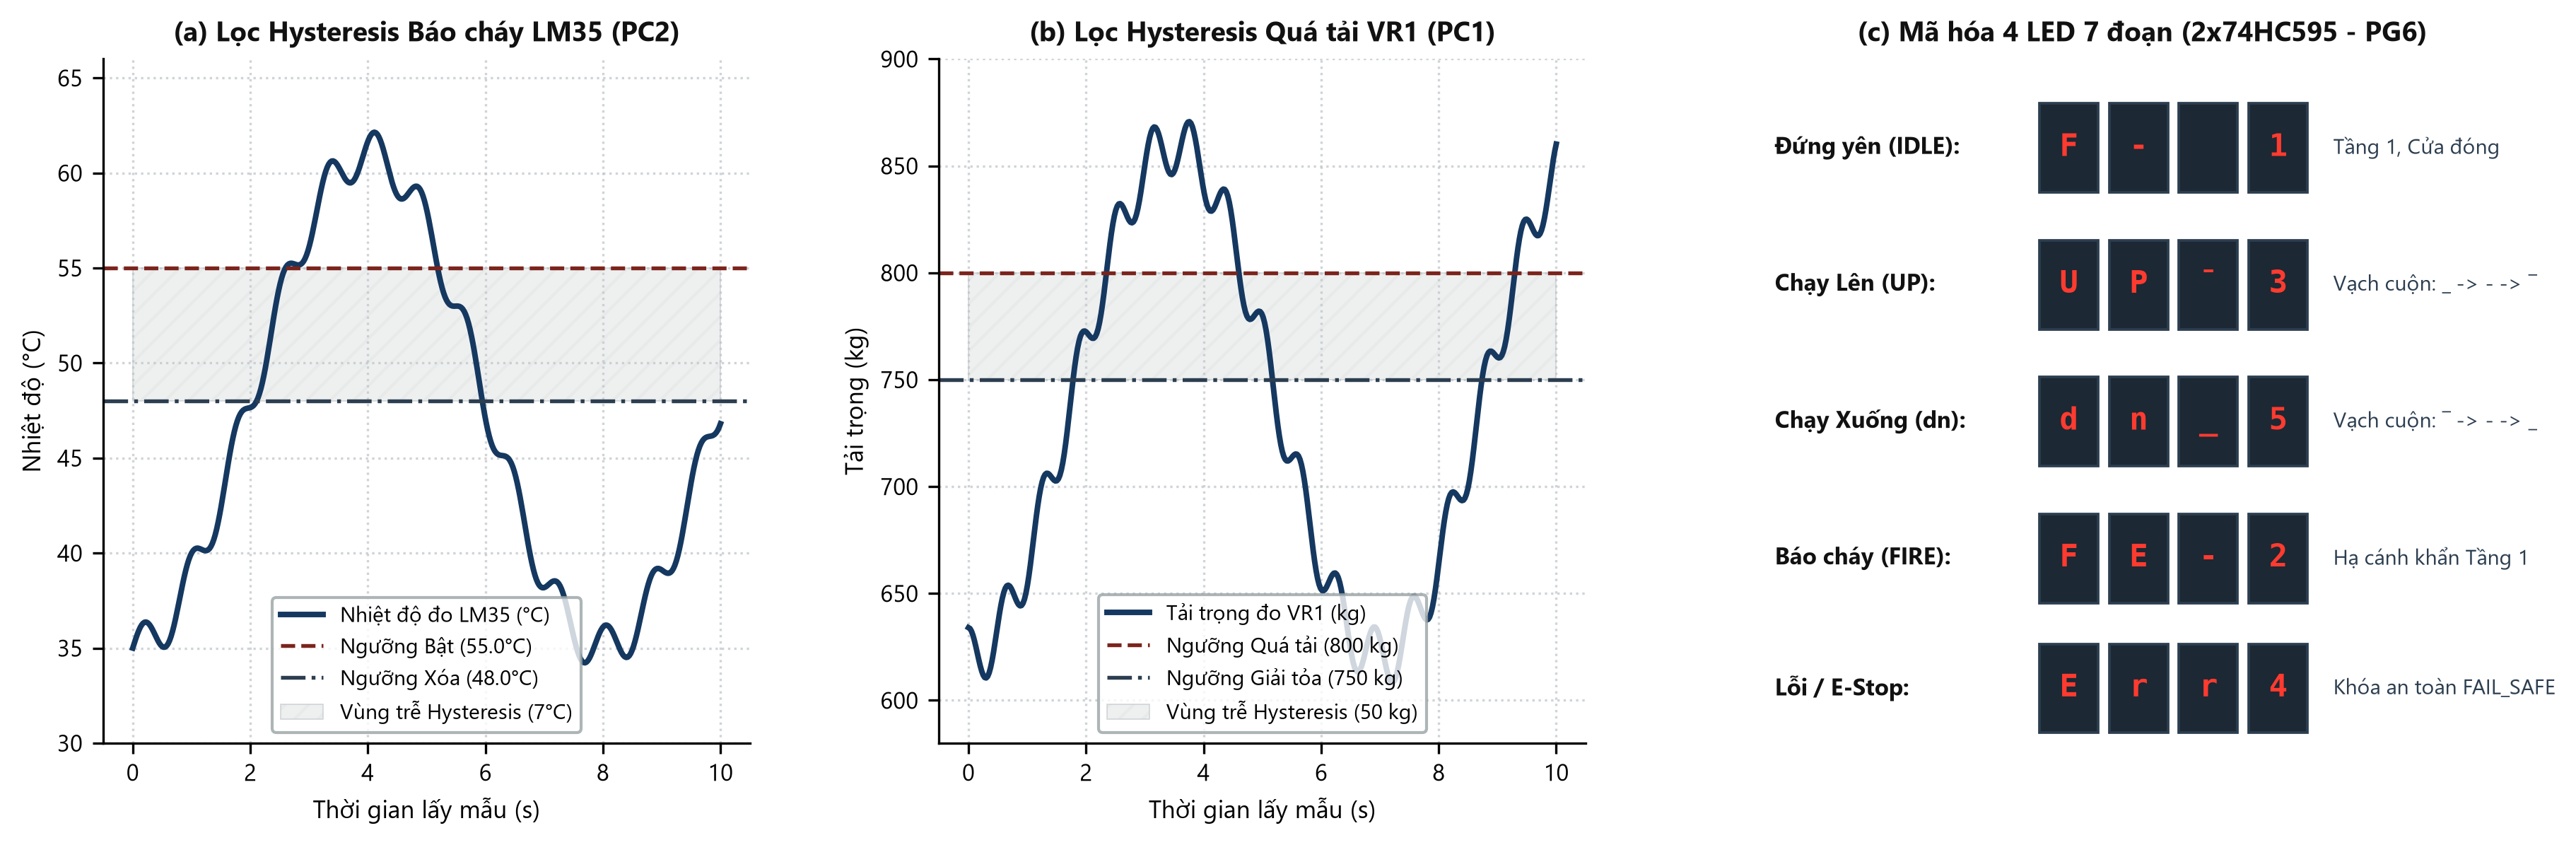
\includegraphics[width=0.99\textwidth]{image/fig_hysteresis_hmi.png}
\caption{Đồ thị đặc tuyến trễ 2 ngưỡng (Hysteresis) của \texttt{LM35} \& \texttt{VR1} và quy tắc mã hóa 4 LED 7 đoạn trên bus \texttt{SPI1}}
\label{fig:hysteresis_hmi}
\end{figure}

\begingroup
\renewcommand{\arraystretch}{1.18}%
\setlength{\tabcolsep}{4.5pt}%
\fontsize{8.2}{10.5}\selectfont
\arrayrulecolor{tableborder}%
\begin{xltabular}{\textwidth}{|C{2.0cm}|L{3.2cm}|L{3.5cm}|Y|}
\caption{Bảng ánh xạ chức năng 16 phím ma trận 4$\times$4 (\texttt{PD3}) và mã hiển thị 4 LED 7 đoạn (\texttt{PG6})}\label{tab:keypad_7seg}\\
\hline
\rowcolor{tablehead}
\thcell{Mã Phím} & \thcell{Sự kiện HSM phát sinh} & \thcell{Chức năng trên Bo mạch} & \thcell{Phản hồi Âm thanh (PF8) \& LED 7 Đoạn (PG6)} \\
\hline
\endfirsthead
\hline
\rowcolor{tablehead}
\thcell{Mã Phím} & \thcell{Sự kiện HSM phát sinh} & \thcell{Chức năng trên Bo mạch} & \thcell{Phản hồi Âm thanh (PF8) \& LED 7 Đoạn (PG6)} \\
\hline
\endhead
\hline
\endfoot
\hline
\endlastfoot
\texttt{Phím 0..6} & \texttt{EV\_CALL\_CABIN (1..7)} & Gọi trực tiếp \textbf{Tầng 1 .. Tầng 7}. & Còi bíp \texttt{2400 Hz (35 ms)}; đưa tầng vào \texttt{cabin\_mask}. \\
\hline
\rowcolor{roweven}
\texttt{Phím 7} & \texttt{EV\_DOOR\_OPEN\_REQ} & Nút \textbf{Mở cửa nhanh (\texttt{<|>})} tại tầng. & Còi bíp \texttt{2400 Hz}; mở lại cửa nếu đang đứng yên/đang đóng. \\
\hline
\texttt{Phím 8} & \texttt{EV\_DOOR\_CLOSE\_REQ} & Nút \textbf{Đóng cửa nhanh (\texttt{>|<})}. & Còi bíp \texttt{2400 Hz}; rút ngắn thời gian giữ mở cửa. \\
\hline
\rowcolor{roweven}
\texttt{Phím 9} & \texttt{EV\_DOOR\_OBSTRUCT\_X0} & Giả lập \textbf{Kẹt cửa (\texttt{X0 -- PA6})}. & Còi cảnh báo kép \texttt{1800 Hz}; đảo chiều mở cửa ngay lập tức. \\
\hline
\texttt{Phím 10} & \texttt{EV\_FIRE\_DETECTED} & Kích hoạt \textbf{Báo cháy khẩn cấp}. & Còi hụ báo cháy \texttt{2800/1800 Hz}; LED hiển thị \texttt{FE- [Tầng]}. \\
\hline
\rowcolor{roweven}
\texttt{Phím 11} & \texttt{EV\_ESTOP\_X1} & Kích hoạt \textbf{Dừng khẩn (\texttt{E-Stop})}. & Còi cảnh báo lỗi; cắt rơ-le \texttt{PE5/PE6}, LED hiển thị \texttt{Err[Tầng]}. \\
\hline
\texttt{Phím 12..15} & \texttt{EV\_FAULT\_CLEAR} & \textbf{Xóa lỗi / Khôi phục (\texttt{CLEAR})}. & Xóa trạng thái \texttt{FIRE\_EVAC / FAIL\_SAFE} về \texttt{IDLE\_CLOSED}. \\
\end{xltabular}
\endgroup

\pagebreak
Đoạn mã nguồn C dưới đây minh họa trực tiếp giải thuật quy đổi điện áp 5 kênh ADC sang các đại lượng vật lý chuẩn trong \texttt{bsp\_adc\_sensors.c} và thuật toán lọc trễ Hysteresis 2 ngưỡng kích hoạt cảnh báo an toàn trong luồng \texttt{t1\_safety}:

\begin{lstlisting}[language=C, caption={Quy đổi ADC 5 kênh (bsp\_adc\_sensors.c) và cơ chế Hysteresis trong t1\_safety (main.c)}]
/* 1. Quy doi dien ap ADC 12-bit sang dai do vat ly (zero-float) */
int bsp_adc_read(bsp_adc_data_t *out) {
    out->temp_deci_c = mv_vals[0]; /* LM35: 10 mV/C -> 0.1 C */
    int32_t load = (mv_vals[1] * (int32_t)ELEV_LOAD_MAX_KG) / 3300;
    out->load_kg = (uint16_t)CLAMP(load, 0, ELEV_LOAD_MAX_KG);
    out->light_mv   = (uint16_t)CLAMP(mv_vals[2], 0, 3300);
    out->bus_mv     = (uint16_t)CLAMP(mv_vals[3], 0, 3300);
    out->current_mv = (uint16_t)CLAMP(mv_vals[4], 0, 3300);
    return any_ok ? 0 : -EIO;
}

/* 2. Bo loc tre Hysteresis 2 nguong trong luong t1_safety */
/* Bao chay: Bat >=55.0 C (550), giai toa khi ha <=48.0 C (480) */
if (!prev_overheat && adc.temp_deci_c >= 550) {
    prev_overheat = true;
    elevator_event_t ev = { .type = EV_OVERHEAT_TEMP,
                            .param = adc.temp_deci_c };
    (void)elevator_hsm_post_event(&ev);
    (void)can_bus_send_emergency(1U, 0U);
} else if (prev_overheat &&
           adc.temp_deci_c <= ELEV_TEMP_CLEAR_THRESH_DC) {
    prev_overheat = false;
    elevator_event_t ev = { .type = EV_TEMP_NORMAL };
    (void)elevator_hsm_post_event(&ev);
}

/* Qua tai: Bat >=800 kg (giu cua), chi xoa khi tai <=750 kg */
if (!prev_overload && ((adc_ok && adc.load_kg >= 800) || x3)) {
    prev_overload = true;
    elevator_event_t ev = { .type = EV_OVERLOAD_SET,
                            .param = adc.load_kg };
    (void)elevator_hsm_post_event(&ev);
} else if (prev_overload && !x3 &&
           (!adc_ok || adc.load_kg <= ELEV_LOAD_CLEAR_KG)) {
    prev_overload = false;
    elevator_event_t ev = { .type = EV_OVERLOAD_CLEAR };
    (void)elevator_hsm_post_event(&ev);
}
\end{lstlisting}

\subsection{Giao thức CAN Bus 500 kbps, Bộ lọc Phần cứng và Cơ chế Fail-Safe}
Nhằm hiện thực hóa mạng truyền thông công nghiệp phân tán có khả năng kháng nhiễu điện từ cao giữa bộ điều khiển cabin và trạm hiển thị hành lang ngoài sảnh, lớp truyền thông tích hợp bộ điều khiển vi mô CAN 2.0A ở tốc độ 500 kbps kết hợp cơ chế tự phục hồi lỗi đường truyền (Hình~\ref{fig:can_eeprom}A và Bảng~\ref{tab:can_frames}):
\begin{itemize}[nosep]
    \item \textbf{Trình tự khởi tạo chuẩn theo Zephyr Driver và Phân bổ CAN ID ưu tiên (\textit{CSMA/AMP}):}
    \begin{itemize}[nosep]
        \item \textit{Trình tự khởi động driver:} Tuân thủ nghiêm ngặt chuỗi gọi hàm tiêu chuẩn của Zephyr CAN API: cấu hình chế độ hoạt động kèm cơ chế phục hồi thủ công qua \texttt{can\_set\_mode(can\_dev, mode | CAN\_MODE\_MANUAL\_RECOVERY)} $\rightarrow$ đăng ký 3 bộ lọc phần cứng vào hàng đợi \texttt{g\_can\_rx\_msgq} bằng \texttt{can\_add\_rx\_filter\_msgq()} $\rightarrow$ kích hoạt bộ điều khiển bằng \texttt{can\_start()}.
        \item \textit{3 bộ lọc chấp nhận phần cứng (Hardware Acceptance Filters):} Tận dụng cơ chế lọc mặt nạ trực tiếp trên thanh ghi của khối \texttt{bxCAN1} để loại bỏ 100\% các khung tin không thuộc phạm vi xử lý mà không làm tiêu tốn chu kỳ CPU:
        \begin{itemize}[nosep]
            \item \textbf{Filter 1 (Mask \texttt{0x7FF}):} Khớp chính xác duy nhất khung khẩn cấp \texttt{0x080} (Dừng khẩn / Báo cháy).
            \item \textbf{Filter 2 (Mask \texttt{0x7F0}):} Khớp dải 16 mã ID \texttt{0x100..0x10F} chuyên dùng nhận các lệnh gọi tầng từ sảnh ngoài.
            \item \textbf{Filter 3 (Mask \texttt{0x600}):} Khớp toàn bộ dải ID \texttt{0x200..0x3FF}, tiếp nhận đồng thời khung trạng thái cabin (\texttt{0x200}), khung nhịp tim Heartbeat định kỳ (\texttt{0x300}), khung kiểm tra độ trễ khứ hồi \texttt{canping} (\texttt{0x380/0x381}) và yêu cầu truyền từ xa (\texttt{RTR}).
        \end{itemize}
        \item \textit{Phân cấp ưu tiên không phá hủy:} Dựa trên đặc tính mức logic '0' có tính trạng thái trội (Dominant Bit) của chuẩn CAN 2.0A, các gói tin có CAN ID nhỏ hơn sẽ luôn chiếm quyền truyền dẫn tức thời. Khung sự cố an toàn (\texttt{0x080}) luôn chiếm ưu thế tuyệt đối trước khung dữ liệu định kỳ (\texttt{0x200/0x300}).
    \end{itemize}
    \item \textbf{Truyền bất đồng bộ kèm Callback, chuẩn hóa Big-Endian và Phản hồi khung \texttt{RTR}:}
    \begin{itemize}[nosep]
        \item Mọi thao tác phát khung tin qua \texttt{can\_send()} đều thiết lập hàm callback bất đồng bộ \texttt{can\_tx\_done\_cb()} với thời gian chờ tối đa 20 ms. Việc truyền diễn ra hoàn toàn không chặn (non-blocking), cập nhật số lượng khung thành công/thất bại qua hai biến đếm nguyên tử \texttt{g\_tx\_ok} và \texttt{g\_tx\_err}.
        \item Toàn bộ dữ liệu nhiều byte (\texttt{uptime\_ms} 32-bit, số thứ tự \texttt{seq} 16-bit, dấu thời gian đo độ trễ \texttt{RTT}) đều được mã hóa tường minh theo định dạng mạng \textbf{Big-Endian} (\texttt{sys\_put\_be32}, \texttt{sys\_put\_be16}), bảo đảm tính tương thích nhị phân tuyệt đối giữa STM32 Cortex-M4 (Little-Endian) và ứng dụng giám sát PC Digital Twin (x86\_64).
        \item Tùy chọn cấu hình \texttt{CONFIG\_CAN\_ACCEPT\_RTR=y} cho phép bộ điều khiển cabin phát hiện và phản hồi ngay lập tức khung trạng thái mới nhất khi trạm sảnh phát tín hiệu truy vấn từ xa \texttt{CAN\_FRAME\_RTR} trên ID \texttt{0x200}.
    \end{itemize}
    \item \textbf{Giám sát mất kết nối 2000~ms và Phục hồi tự động khỏi trạng thái \texttt{BUS-OFF}:}
    \begin{itemize}[nosep]
        \item \textit{Watchdog đối tác (\texttt{t3\_can\_wdt}):} Luồng chuyên trách ngủ trên lệnh nhận semaphore \texttt{k\_sem\_take(\&g\_can\_partner\_sem, K\_MSEC(2000))}. Khi đối tác mất nguồn hoặc cáp truyền thông bị đứt quá 2000 ms, hàm trả về lỗi \texttt{-EAGAIN}. Hệ thống chốt cờ lỗi đường truyền \texttt{g\_link\_fault\_latched}, hủy bỏ chế độ hiển thị từ xa và phát sự kiện \texttt{EV\_CAN\_LINK\_LOST} đưa thang máy vào trạng thái an toàn \texttt{HSM\_STATE\_FAIL\_SAFE}.
        \item \textit{Tự động thoát lỗi BUS-OFF:} Khi bộ đếm lỗi truyền \texttt{TEC} vượt quá ngưỡng 255 do đoản mạch hoặc xung nhiễu lớn, phần cứng tự động cô lập bộ thu phát (\texttt{CAN\_STATE\_BUS\_OFF}). Trong luồng \texttt{t3\_can\_tx}, hệ thống định kỳ kiểm tra trạng thái bus; nếu phát hiện \texttt{BUS-OFF}, hệ thống ghi mã sự cố \texttt{BB\_FAULT\_CAN\_BUS\_OFF} vào hộp đen EEPROM, giới hạn tần suất xử lý (tối đa 1 lần/giây) và kích hoạt hàm phục hồi Zephyr \texttt{can\_recover(can\_dev, K\_MSEC(100))} để kéo bộ điều khiển trở lại mạng.
    \end{itemize}
\end{itemize}

\begin{figure}[H]
\centering
\resizebox{\textwidth}{!}{%
\begin{tikzpicture}
    % === PHAN A: 3 BO LOC PHAN CUNG bxCAN1 (500 kbps) ===
    \node[font=\footnotesize\bfseries, text=tablehead, anchor=west] at (0, 5.75)
        {(a) Phân hoạch Ưu tiên 11-bit (\textit{CSMA/AMP}) và 3 Bộ lọc Chấp nhận Phần cứng \texttt{bxCAN1} (\texttt{500 kbps})};

    \node[acadbox, text width=4.85cm, minimum height=1.80cm] (F1) at (2.55, 4.40)
        {\textbf{HW Filter 1 -- Mức Khẩn cấp}\\[1pt]
         {\tiny \texttt{ID = 0x080 | Mask = 0x7FF}}\\[2pt]
         {\tiny Thắng phân xử bit tuyệt đối trên bus\\
         \texttt{DLC=2}: [\texttt{Mã E-Stop/Fire}, \texttt{Tầng}]}};

    \node[acadbox, text width=4.85cm, minimum height=1.80cm] (F2) at (7.90, 4.40)
        {\textbf{HW Filter 2 -- Gọi tầng Hành lang}\\[1pt]
         {\tiny \texttt{ID = 0x100..0x10F | Mask = 0x7F0}}\\[2pt]
         {\tiny Gom lệnh gọi nút \texttt{HALL} về \texttt{CABIN}\\
         \texttt{DLC=2}: [\texttt{Tầng 1..7}, \texttt{UP/DOWN}]}};

    \node[acadbox, text width=4.85cm, minimum height=1.80cm] (F3) at (13.25, 4.40)
        {\textbf{HW Filter 3 -- Giám sát \& Đo RTT}\\[1pt]
         {\tiny \texttt{ID = 0x200..0x3FF | Mask = 0x600}}\\[2pt]
         {\tiny \texttt{0x200} Status (\texttt{RTR}) $\cdot$ \texttt{0x300} HB \texttt{250ms}\\
         \texttt{0x380/0x381} Khung đo \texttt{PING/PONG}}};

    % === PHAN B: TO CHUC BO NHO AT24C512 EEPROM (64 KB, Trang 128 B) ===
    \node[font=\footnotesize\bfseries, text=tablehead, anchor=west] at (0, 2.75)
        {(b) Sơ đồ Ánh xạ Vùng nhớ Hộp đen Vòng 32 Bản ghi trên \texttt{AT24C512 EEPROM} (\texttt{I2C1 0x50}, Trang \texttt{128 Byte})};

    \node[acadboxnav, text width=4.25cm, minimum height=1.85cm] (HDR) at (2.25, 1.25)
        {\textbf{Khối Header Quản lý}\\[1pt]
         {\tiny Địa chỉ \texttt{0x0000} (16 Bytes)}\\[2pt]
         {\tiny \texttt{magic = 0x454C4556 ("ELEV")}\\
         \texttt{next\_seq}, \texttt{write\_idx}, \texttt{valid\_cnt}\\
         Toàn vẹn: \texttt{crc32\_ieee} (4 Bytes)}};

    \node[acadbox, text width=5.65cm, minimum height=1.85cm] (RING) at (7.80, 1.25)
        {\textbf{Hàng đợi Vòng 32 Bản ghi Sự cố}\\[1pt]
         {\tiny Địa chỉ \texttt{0x0080 + idx * 32} (\texttt{STRIDE = 32 B})}\\[2pt]
         {\tiny Gói \texttt{elevator\_blackbox\_rec\_t} (22 Bytes packed)\\
          Nằm gọn trang \texttt{128 B}, chống xé trang I2C}};

    \node[acadbox, text width=4.35cm, minimum height=1.85cm] (REC) at (13.45, 1.25)
        {\textbf{Cơ chế An toàn \& Phục hồi}\\[1pt]
         {\tiny Tự ghi hộp đen khi xảy ra:}\\[2pt]
         {\tiny $\bullet$ \texttt{IWDG Reset} (2500ms) qua \texttt{HWINFO}\\
         $\bullet$ \texttt{CAN\_LINK\_LOST} (>2000ms)\\
         $\bullet$ \texttt{BUS-OFF} $\rightarrow$ \texttt{can\_recover()}}};

    \draw[acadarr] (HDR.east) -- (RING.west);
    \draw[acadarr] (REC.west) -- (RING.east);

    % Thanh chi tiet tung truong cua 1 ban ghi 22-byte packed ben trong 32-byte stride
    \node[font=\tiny\bfseries, text=black!80, anchor=west] at (0, -0.35)
        {Chi tiết phân bổ trường bên trong 1 bản ghi \texttt{elevator\_blackbox\_rec\_t} (địa chỉ tương đối \texttt{+0x00 .. +0x15}):};

    \draw[acadline, fill=black!3] (0.0, -1.45) rectangle (2.1, -0.70);
    \node[align=center, font=\tiny] at (1.05, -1.07) {\texttt{+0..3} (4B)\\\texttt{seq}};

    \draw[acadline, fill=white] (2.1, -1.45) rectangle (4.3, -0.70);
    \node[align=center, font=\tiny] at (3.20, -1.07) {\texttt{+4..7} (4B)\\\texttt{uptime\_ms}};

    \draw[acadline, fill=black!3] (4.3, -1.45) rectangle (7.6, -0.70);
    \node[align=center, font=\tiny] at (5.95, -1.07) {\texttt{+8..14} (7B)\\Giờ \texttt{DS3231} (\texttt{Y,M,D,h,m,s})};

    \draw[acadline, fill=white] (7.6, -1.45) rectangle (9.5, -0.70);
    \node[align=center, font=\tiny] at (8.55, -1.07) {\texttt{+15} (1B)\\\texttt{fault\_code}};

    \draw[acadline, fill=black!3] (9.5, -1.45) rectangle (11.4, -0.70);
    \node[align=center, font=\tiny] at (10.45, -1.07) {\texttt{+16..17} (2B)\\\texttt{state}, \texttt{floor}};

    \draw[acadline, fill=white] (11.4, -1.45) rectangle (13.6, -0.70);
    \node[align=center, font=\tiny] at (12.50, -1.07) {\texttt{+18..19} (2B)\\\texttt{temp\_deci\_c}};

    \draw[acadline, fill=tablehead!12] (13.6, -1.45) rectangle (15.80, -0.70);
    \node[align=center, font=\tiny] at (14.70, -1.07) {\texttt{+20..21} (2B)\\\textbf{\texttt{crc16\_ccitt}}};
\end{tikzpicture}%
}

\caption{Kiến trúc 3 bộ lọc phần cứng \texttt{bxCAN 500 kbps} và cấu trúc vùng nhớ hộp đen vòng 32 bản ghi trên \texttt{AT24C512 EEPROM}}
\label{fig:can_eeprom}
\end{figure}

\begingroup
\renewcommand{\arraystretch}{1.18}%
\setlength{\tabcolsep}{4pt}%
\fontsize{8.1}{10.4}\selectfont
\arrayrulecolor{tableborder}%
\begin{xltabular}{\textwidth}{|C{1.45cm}|C{2.1cm}|C{1.1cm}|C{1.9cm}|Y|}
\caption{Đặc tả tập khung truyền mạng CAN Bus 500 kbps và cấu trúc Payload (Big-Endian)}\label{tab:can_frames}\\
\hline
\rowcolor{tablehead}
\thcell{CAN ID} & \thcell{Bộ lọc Phần cứng} & \thcell{DLC} & \thcell{Chu kỳ / Kiểu} & \thcell{Định dạng Byte Payload (Big-Endian) \& Ý nghĩa} \\
\hline
\endfirsthead
\hline
\rowcolor{tablehead}
\thcell{CAN ID} & \thcell{Bộ lọc Phần cứng} & \thcell{DLC} & \thcell{Chu kỳ / Kiểu} & \thcell{Định dạng Byte Payload (Big-Endian) \& Ý nghĩa} \\
\hline
\endhead
\hline
\endfoot
\hline
\endlastfoot
\texttt{0x080} & Filter 1 (\texttt{0x7FF}) & 3~B & Sự kiện khẩn & \texttt{B0}: Mã lỗi (\texttt{1=Fire, 2=E-Stop}); \texttt{B1}: Tầng; \texttt{B2}: \texttt{0xFF}. \\
\hline
\rowcolor{roweven}
\texttt{0x10x} & Filter 2 (\texttt{0x7F0}) & 2~B & Khi bấm gọi & \texttt{B0}: Tầng gọi (\texttt{1..7}); \texttt{B1}: Hướng gọi (\texttt{1=UP, 0=DOWN}). \\
\hline
\texttt{0x200} & Filter 3 (\texttt{0x600}) & 8~B & 250~ms / \texttt{RTR} & \texttt{B0}: State; \texttt{B1}: Tầng; \texttt{B2}: Đích; \texttt{B3}: Dir+1; \texttt{B4}: Cửa\%; \texttt{B5}: Flags; \texttt{B6..7}: Mask. \\
\hline
\rowcolor{roweven}
\texttt{0x300} & Filter 3 (\texttt{0x600}) & 8~B & 250~ms (Định kỳ) & \texttt{B0}: Role (\texttt{0xA5/0x5A}); \texttt{B1}: State; \texttt{B2..5}: \texttt{uptime\_ms} (BE32); \texttt{B6..7}: \texttt{seq} (BE16). \\
\hline
\texttt{0x380} & Filter 3 (\texttt{0x600}) & 8~B & Lệnh \texttt{canping} & Khung \textbf{PING} chứa \texttt{seq} (\texttt{BE32}) và \texttt{uptime\_ms} (\texttt{BE32}). \\
\hline
\rowcolor{roweven}
\texttt{0x381} & Filter 3 (\texttt{0x600}) & 8~B & Phản hồi tức thời & Khung \textbf{PONG} hoàn trả payload để tính độ trễ khứ hồi \texttt{RTT} qua DWT. \\
\end{xltabular}
\endgroup

\pagebreak
Đoạn mã nguồn C trích từ \texttt{src/comms/can\_bus.c} dưới đây minh họa chi tiết quá trình thiết lập 3 bộ lọc phần cứng trên bộ điều khiển \texttt{bxCAN1}, vòng lặp giám sát liên kết truyền thông 2000~ms và cơ chế tự động phục hồi khỏi lỗi \texttt{BUS-OFF}:

\begin{lstlisting}[language=C, caption={Cấu hình 3 bộ lọc phần cứng (can\_bus.c) và giám sát liên kết CAN 2000~ms (t3\_can\_wdt)}]
/* 1. Cai dat 3 bo loc chap nhan phan cung tren bxCAN1 */
static int install_hw_filters(void) {
    /* Filter 1: 0x080 E-Stop (mask 0x7FF) */
    const struct can_filter f1 = {
        .id = CAN_ID_EMERGENCY_STOP, .mask = 0x7FFU
    };
    /* Filter 2: 0x100..0x10F Hall Calls (mask 0x7F0) */
    const struct can_filter f2 = {
        .id = CAN_ID_HALL_CALL, .mask = 0x7F0U
    };
    /* Filter 3: 0x200..0x3FF Cabin Status (mask 0x600) */
    const struct can_filter f3 = {
        .id = CAN_ID_CABIN_STATUS, .mask = 0x600U
    };
    int id1 = can_add_rx_filter_msgq(can_dev, &g_can_rx_msgq, &f1);
    int id2 = can_add_rx_filter_msgq(can_dev, &g_can_rx_msgq, &f2);
    int id3 = can_add_rx_filter_msgq(can_dev, &g_can_rx_msgq, &f3);
    return (id1 >= 0 && id2 >= 0 && id3 >= 0) ? 0 : -ENOSPC;
}

/* 2. Giam sat nhip tim doi tac voi timeout 2000 ms (t3_can_wdt) */
void can_bus_partner_watchdog_step(void) {
    int err = k_sem_take(&g_can_partner_sem,
                         K_MSEC(ELEV_CAN_TIMEOUT_MS));
    if (err == -EAGAIN) { /* Qua 2000 ms mat heartbeat */
        k_mutex_lock(&g_can_state_mutex, K_FOREVER);
        bool first_fault = !g_link_fault_latched;
        if (first_fault) {
            g_link_fault_latched = true;
            g_remote_valid = false;
        }
        k_mutex_unlock(&g_can_state_mutex);
        if (first_fault) {
            elevator_event_t ev = { .type = EV_CAN_LINK_LOST };
            (void)elevator_hsm_post_event(&ev);
        }
    }
}

/* 3. Phat hien BUS-OFF, ghi hop den va can_recover() */
if (state == CAN_STATE_BUS_OFF &&
    (now_ms - g_last_recover_ms) > 1000U) {
    g_last_recover_ms = now_ms;
    LOG_ERR("CAN BUS-OFF (TEC=%u) -> recover", cnt.tx_err_cnt);
    (void)bsp_blackbox_append(BB_FAULT_CAN_BUS_OFF,
                              HSM_STATE_FAIL_SAFE, 0U, 0);
    (void)can_recover(can_dev, K_MSEC(100));
}
\end{lstlisting}

\subsection{Hộp đen EEPROM AT24C512, Hardware Watchdog và Kết quả Biên dịch}
Nhằm đảm bảo khả năng tự giám sát độ sống của toàn bộ các luồng phần mềm, lưu trữ bất khả biến các biến cố an toàn và đánh giá hiệu năng tối ưu tài nguyên của hệ thống, firmware tích hợp bộ đếm Independent Watchdog, hệ thống hộp đen EEPROM hai tầng kiểm tra toàn vẹn và thực hiện đo lường bộ nhớ lúc biên dịch (Hình~\ref{fig:can_eeprom}B và Bảng~\ref{tab:eeprom_layout}):
\begin{itemize}[nosep]
    \item \textbf{Giám sát độ sống đa luồng qua Hardware Watchdog (\textmd{\texttt{IWDG}}) và Định danh nguyên nhân khởi động:}
    \begin{itemize}[nosep]
        \item \textit{Nguyên tắc điểm danh đa luồng (\texttt{bsp\_wdt\_checkin}):} Bộ đếm thời gian độc lập IWDG trên STM32F407 vận hành từ nguồn xung nội bộ LSI ($\sim 32\text{ kHz}$) độc lập hoàn toàn với mạch dao động chính, với ngưỡng tràn ngắt cứng là 2500 ms. Để ngăn ngừa hiện tượng một luồng đơn lẻ còn chạy tiếp tục nuôi watchdog trong khi các luồng khác đã bị treo chết (deadlock), hệ thống thiết lập cơ chế kiểm tra chéo: cả 4 luồng trọng yếu (\texttt{t1\_safety}, \texttt{t2\_fsm}, \texttt{t3\_can\_tx}, \texttt{t4\_hmi}) đều bắt buộc phải định kỳ gọi hàm \texttt{bsp\_wdt\_checkin(id)} để cập nhật mốc thời gian sống.
        \item \textit{Dịch vụ nạp Watchdog (\texttt{bsp\_wdt\_service}):} Luồng giám sát \texttt{t5\_wdt} định kỳ mỗi 100 ms quét mảng mốc thời gian của 4 luồng dưới sự bảo vệ của khóa quay \texttt{k\_spinlock} (\texttt{g\_wdt\_lock}). Chỉ khi toàn bộ 4 luồng đều có thời gian phản hồi trong vòng \texttt{THREAD\_STALL\_TIMEOUT\_MS = 1500 ms} gần nhất, hàm mới thực thi lệnh \texttt{wdt\_feed()}. Nếu bất kỳ luồng nào bị treo quá 1500 ms, lệnh nạp bị khóa hoàn toàn, buộc phần cứng kích hoạt reset hệ thống sau đúng 2500 ms.
        \item \textit{Định danh nguyên nhân khởi động qua \texttt{HWINFO}:} Ngay khi CPU khởi động lại, hàm \texttt{bsp\_watchdog\_init} kiểm tra cờ nguyên nhân qua \texttt{hwinfo\_get\_\allowbreak reset\_\allowbreak cause()}. Nếu phát hiện cờ \texttt{RESET\_\allowbreak WATCHDOG} (do IWDG kích hoạt), firmware lập tức ghi bản ghi sự cố \texttt{BB\_FAULT\_\allowbreak BOOT\_\allowbreak WATCHDOG} vào hộp đen EEPROM rồi gọi \texttt{hwinfo\_clear\_\allowbreak reset\_\allowbreak cause()}, giúp phân biệt rạch ròi giữa khởi động cấp nguồn và khởi động khôi phục lỗi treo.
    \end{itemize}
    \item \textbf{Hộp đen vòng 32 bản ghi trên AT24C512 EEPROM với IC thời gian thực DS3231:}
    \begin{itemize}[nosep]
        \item \textit{Phần cứng lưu trữ chuyên dụng:} Hệ thống khai thác chip nhớ EEPROM I2C \textbf{AT24C512} (dung lượng 64 KB, tổ chức theo trang vật lý 128 Byte) kết hợp chip đồng hồ thời gian thực \textbf{DS3231} (độ chính xác $\pm 2\text{ ppm}$, có pin CMOS dự phòng) trên cùng bus \texttt{I2C1} được bảo vệ bởi khóa kế thừa độ ưu tiên \texttt{g\_i2c1\_bus\_mutex}.
        \item \textit{Cấu trúc bản ghi và Căn chỉnh trang an toàn:} Mỗi bản ghi sự cố \texttt{elevator\_\allowbreak blackbox\_\allowbreak rec\_t} có kích thước nén 22 Byte và bước nhảy địa chỉ cố định \texttt{BB\_REC\_STRIDE = 32 Bytes}. Vùng nhớ 32 bản ghi (địa chỉ \texttt{0x0080..0x047F}) được thiết kế sao cho mỗi trang 128 Byte của EEPROM chứa trọn vẹn đúng 4 bản ghi, triệt tiêu hoàn toàn rủi ro ghi tràn biên trang vật lý (Page-boundary Wrap-around).
        \item \textit{Toàn vẹn dữ liệu hai tầng (\textit{Two-Tier Integrity}):} Khối thông tin đầu trang (\textit{Header}) tại \texttt{0x0000} quản lý \texttt{magic} (\texttt{0x424B4954}), con trỏ ghi xoay vòng \texttt{write\_idx}, số bản ghi hợp lệ \texttt{valid\_count} và số thứ tự đơn điệu \texttt{next\_seq}, được bảo vệ bởi mã băm kiểm tra \textbf{CRC32-IEEE}. Từng bản ghi sự cố tại \texttt{0x0080 + idx * 32} lưu trữ đầy đủ dấu thời gian thực (Năm, Tháng, Ngày, Giờ, Phút, Giây), mã lỗi, trạng thái HSM, tầng và nhiệt độ, được bảo vệ riêng bằng mã \textbf{CRC16-CCITT} (đa thức \texttt{0x1021}).
        \item \textit{Quy trình ghi bất đối xứng an toàn mất điện:} Firmware luôn ghi toàn bộ cấu trúc bản ghi mới xuống vùng nhớ ô dữ liệu trước; chỉ khi giao dịch I2C thành công mới cập nhật con trỏ \texttt{write\_idx} và tính lại \texttt{CRC32} ghi xuống Header, đảm bảo dữ liệu lịch sử không bao giờ bị hỏng nếu nguồn điện đột ngột bị ngắt giữa chừng.
    \end{itemize}
    \item \textbf{Kết quả biên dịch thực tế trên Zephyr SDK v1.0.1 (arm-zephyr-eabi-gcc 14.3.0):}
    \begin{itemize}[nosep]
        \item \textit{Độ tin cậy mã nguồn:} Toàn bộ 18 mục tiêu (bao gồm cả nhân Zephyr, driver BSP, máy trạng thái Core, mạng CAN và giao diện dòng lệnh CLI) đều được biên dịch thành công tuyệt đối: \textbf{0 lỗi (\texttt{0 errors}), 0 cảnh báo (\texttt{0 warnings})} ở mức cờ cảnh báo cao nhất \texttt{-Wall -Wextra}.
        \item \textit{Bộ nhớ chương trình (Flash ROM):} Chiếm dụng \textbf{104\,112 Bytes} trên tổng số 1\,048\,576 Bytes khả dụng (\textbf{9.93\%}), để lại hơn 900 KB dự phòng cho việc mở rộng thuật toán điều phối đa cabin và nạp firmware qua mạng (OTA).
        \item \textit{Bộ nhớ dữ liệu tĩnh (SRAM):} Chiếm dụng \textbf{28\,608 Bytes} trên tổng số 131\,072 Bytes (\textbf{21.83\%}). Toàn bộ 100\% biến nhớ và ngăn xếp luồng RTOS đều được cấp phát tĩnh lúc biên dịch (Zero Heap Dynamic Allocation), triệt tiêu hoàn toàn lỗi tràn bộ nhớ hoặc phân mảnh RAM trong các chu kỳ vận hành dài hạn.
    \end{itemize}
\end{itemize}

\begingroup
\renewcommand{\arraystretch}{1.18}%
\setlength{\tabcolsep}{4.5pt}%
\fontsize{8.2}{10.5}\selectfont
\arrayrulecolor{tableborder}%
\begin{xltabular}{\textwidth}{|C{2.0cm}|L{3.1cm}|C{2.1cm}|Y|}
\caption{Cấu trúc bản ghi sự cố (\texttt{elevator\_blackbox\_rec\_t}, bước 32-Byte) trên \texttt{AT24C512 EEPROM}}\label{tab:eeprom_layout}\\
\hline
\rowcolor{tablehead}
\thcell{Offset Byte} & \thcell{Tên Trường} & \thcell{Kiểu Dữ liệu} & \thcell{Mô tả Kỹ thuật \& Cơ chế Kiểm tra Toàn vẹn} \\
\hline
\endfirsthead
\hline
\rowcolor{tablehead}
\thcell{Offset Byte} & \thcell{Tên Trường} & \thcell{Kiểu Dữ liệu} & \thcell{Mô tả Kỹ thuật \& Cơ chế Kiểm tra Toàn vẹn} \\
\hline
\endhead
\hline
\endfoot
\hline
\endlastfoot
\texttt{Byte +0..+3} & \texttt{seq} & \texttt{uint32\_t} & Số thứ tự bản ghi tăng dần đơn điệu dùng để khôi phục thứ tự vòng đệm. \\
\hline
\rowcolor{roweven}
\texttt{Byte +4..+7} & \texttt{uptime\_ms} & \texttt{uint32\_t} & Thời gian hoạt động liên tục tính bằng mili-giây từ lúc MCU cấp nguồn. \\
\hline
\texttt{Byte +8..+14} & \texttt{year..sec} & \texttt{uint16\_t+5B} & Dấu thời gian thực (Năm, Tháng, Ngày, Giờ, Phút, Giây) đọc từ IC \textbf{DS3231} (\texttt{0x68}). \\
\hline
\rowcolor{roweven}
\texttt{Byte +15..+17} & \texttt{fault, state, floor} & \texttt{uint8\_t[3]} & Mã sự cố (\texttt{FIRE, OVERLOAD, OBSTRUCT, ESTOP, CAN\_LOST, WDT}), HSM state \& Tầng. \\
\hline
\texttt{Byte +18..+19} & \texttt{temp\_deci\_c} & \texttt{int16\_t} & Nhiệt độ cảm biến \texttt{LM35 (PC2)} tại thời điểm xảy ra sự cố (đơn vị $0.1^\circ\text{C}$). \\
\hline
\rowcolor{roweven}
\texttt{Byte +20..+21} & \texttt{crc16} & \texttt{uint16\_t} & Mã kiểm tra \textbf{CRC16-CCITT} (đa thức \texttt{0x1021}) tính trên 20 byte đầu của bản ghi. \\
\end{xltabular}
\endgroup

\pagebreak
Đoạn mã nguồn C trích từ \texttt{src/bsp/bsp\_watchdog.c} và \texttt{src/bsp/bsp\_i2c\_storage.c} sau đây minh họa thuật toán điểm danh 4 luồng trước khi nạp IWDG phần cứng và kỹ thuật ghi hộp đen xoay vòng bảo đảm toàn vẹn khi mất điện:

\begin{lstlisting}[language=C, caption={Dịch vụ Watchdog đa luồng (bsp\_watchdog.c) và ghi hộp đen an toàn (bsp\_i2c\_storage.c)}]
/* 1. Kiem tra 4 luong truoc khi nap IWDG (bsp_watchdog.c) */
bool bsp_wdt_service(bool force_freeze) {
    if (force_freeze || !g_wdt_ready) { return false; }
    int64_t now = k_uptime_get();
    k_spinlock_key_t key = k_spin_lock(&g_wdt_lock);
    for (size_t i = 0; i < WDT_MON_COUNT; i++) {
        if ((now - g_last_checkin_ms[i]) > 1500) {
            k_spin_unlock(&g_wdt_lock, key);
            LOG_ERR("WDT STALL: %s", bsp_wdt_slot_name(i));
            return false;
        }
    }
    k_spin_unlock(&g_wdt_lock, key);
    return (wdt_feed(wdt_dev, g_wdt_channel_id) == 0);
}

/* 2. Ghi hop den vong 32 ban ghi vao AT24C512 EEPROM (I2C1) */
int bsp_blackbox_append(blackbox_fault_code_t code,
                        elevator_state_t state,
                        uint8_t floor, int32_t temp_deci_c) {
    struct bb_header hdr = { 0 };
    elevator_blackbox_rec_t rec = { 0 };
    (void)bsp_rtc_get_datetime(&rec.year, &rec.month, &rec.day,
                               &rec.hour, &rec.min, &rec.sec);
    rec.seq = hdr.next_seq++; rec.fault_code = (uint8_t)code;
    rec.state = (uint8_t)state; rec.floor = floor;
    rec.temp_deci_c = (int16_t)temp_deci_c;
    rec.crc16 = bb_rec_crc(&rec); /* CRC16 tren 20 byte */

    k_mutex_lock(&g_i2c1_bus_mutex, K_FOREVER);
    off_t off = (off_t)(BB_REC_BASE_OFFSET +
                        hdr.write_idx * BB_REC_STRIDE);
    int err = eeprom_write(eeprom_dev, off, &rec, sizeof(rec));
    if (err == 0) {
        hdr.write_idx = (uint16_t)((hdr.write_idx + 1U) % 32U);
        hdr.crc32 = bb_hdr_crc(&hdr); /* CRC32 */
        err = eeprom_write(eeprom_dev, BB_HDR_OFFSET, &hdr, sizeof(hdr));
    }
    k_mutex_unlock(&g_i2c1_bus_mutex);
    return err;
}
\end{lstlisting}

\clearpage
\section{THỰC NGHIỆM VÀ ĐÁNH GIÁ KẾT QUẢ}

\subsection{Môi trường Kiểm thử Kép: Zephyr Shell CLI và PC Digital Twin / HIL}
Nhằm đánh giá toàn diện hành vi thời gian thực và kiểm chứng nghiêm ngặt cả 12 yêu cầu kỹ thuật (\texttt{REQ-001..REQ-012}) theo chuẩn chữ V (V-Model Verification \& Validation), hệ thống thiết lập kiến trúc kiểm thử kết hợp giữa \textbf{Đồng mô phỏng Phần cứng trong Vòng lặp (Hardware-in-the-Loop -- HIL Co-Simulation)} và tương tác dòng lệnh trực tiếp \textbf{Zephyr Shell CLI} qua giao tiếp nối tiếp \texttt{USART1 RS232} (\texttt{115200 8N1}) như minh họa tại Hình~\ref{fig:digital_twin_gui} và Bảng~\ref{tab:cli_commands}:
\begin{itemize}[nosep]
    \item \textbf{Tập lệnh chẩn đoán ngoại vi độc lập (\texttt{bkit *} trong \texttt{cli\_bkit\_test.c}):} Cho phép kỹ sư kiểm tra sức khỏe vật lý độc lập của toàn bộ 13 cụm linh kiện trên bo mạch BKIT ARM4 (đọc điện áp 5 kênh ADC1, kiểm tra các chân GPIO Opto \texttt{X0..X3}, quét hiển thị chuỗi ký tự trên 4 LED 7 đoạn, đọc bàn phím ma trận 16 phím, đồng bộ giờ chip RTC \textbf{DS3231}, đọc mã JEDEC ID chip SPI Flash \textbf{W25Q64FV}, đo độ trễ khứ hồi \texttt{CAN RTT} và thống kê dung lượng Stack 7 luồng) hoàn toàn độc lập với trạng thái của thang máy.
    \item \textbf{Tập lệnh điều khiển và tiêm lỗi HIL (\texttt{elev *} trong \texttt{cli\_elev.c}):} Hỗ trợ kích hoạt trực tiếp các thao tác nghiệp vụ: gọi tầng hai chiều (\texttt{elev call}), đóng/mở cửa cưỡng bức (\texttt{elev door}), tiêm các sự cố an toàn khẩn cấp (\texttt{elev fault} \texttt{<fire}\allowbreak\texttt{|ovl}\allowbreak\texttt{|estop}\allowbreak\texttt{|can\_drop}\allowbreak\texttt{|clear>}), chuyển đổi linh hoạt vai trò nút mạng CAN (\texttt{cabin/hall}), xuất ma trận độ phủ chuyển tiếp trạng thái $9\times 9$ (\texttt{elev coverage}) và trích xuất lịch sử 32 bản ghi hộp đen EEPROM (\texttt{elev log}).
    \item \textbf{Phần mềm Bản sao số PC Digital Twin (\texttt{pc\_hil\_twin/elevator\_twin.py}):}
    \begin{itemize}[nosep]
        \item Hiển thị trực quan toàn bộ không gian giếng thang 7 tầng, tọa độ cabin di chuyển mượt mà, độ mở cửa buồng thang tuyến tính $0..100\%$, bảng 4 LED 7 đoạn mô phỏng hướng \texttt{UP/dn} kèm vạch cuộn, đồ thị giám sát nhiệt độ \texttt{LM35} và tải trọng \texttt{VR1} theo thời gian thực từ luồng gói tin JSON \texttt{\$TWIN} (chu kỳ truyền \texttt{200~ms}).
        \item Cung cấp 2 chế độ làm việc: Chế độ kết nối trực tiếp bo mạch thật (\textit{Live RS232 Co-Simulation}) và Chế độ giả lập độc lập (\textit{Offline Simulator}), tích hợp sẵn bộ kịch bản kiểm thử tự động (\textit{HIL Smoke Suite}) và tính năng xuất nhật ký ra tệp định dạng \texttt{.csv}.
    \end{itemize}
\end{itemize}

\begin{figure}[H]
\centering
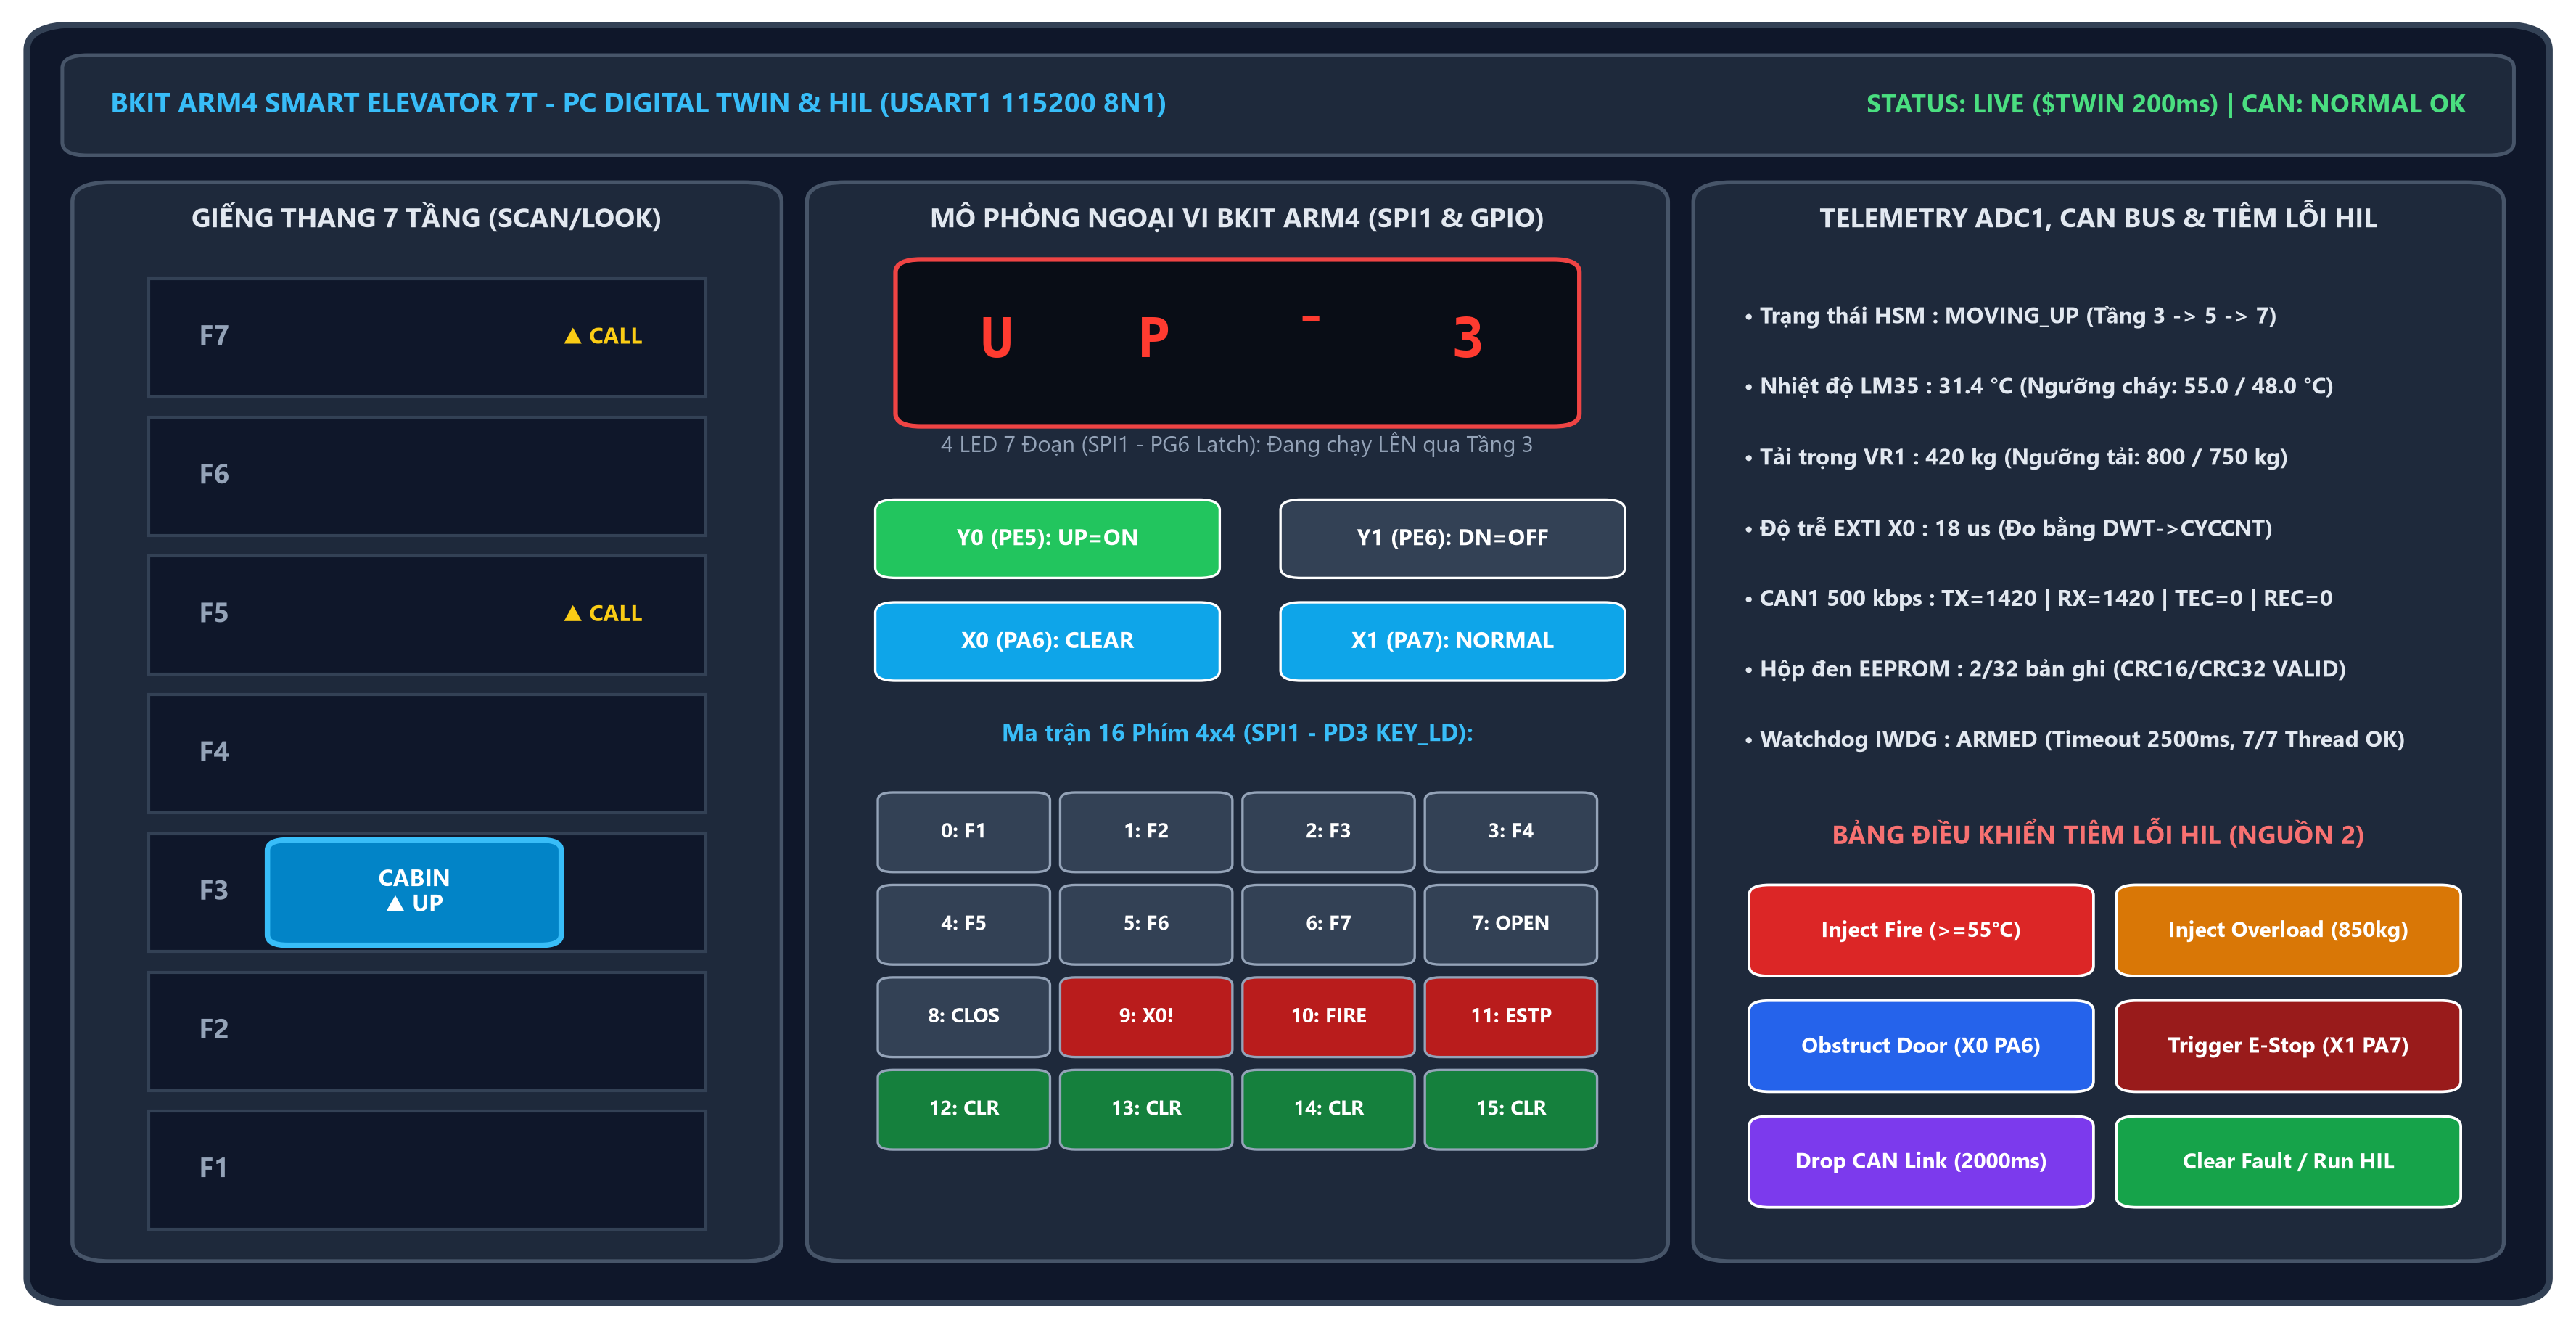
\includegraphics[width=0.99\textwidth]{image/fig_digital_twin_gui.png}
\caption{Giao diện phần mềm Bản sao số PC Digital Twin \& HIL Simulator (\texttt{elevator\_\allowbreak twin.py}) khi đang vận hành và giám sát}
\label{fig:digital_twin_gui}
\end{figure}

\begingroup
\renewcommand{\arraystretch}{1.18}%
\setlength{\tabcolsep}{4.5pt}%
\fontsize{8.1}{10.4}\selectfont
\arrayrulecolor{tableborder}%
\begin{xltabular}{\textwidth}{|L{4.1cm}|L{2.5cm}|Y|}
\caption{Tổng hợp tập lệnh chẩn đoán ngoại vi (\texttt{bkit *}) và điều khiển / tiêm lỗi HIL (\texttt{elev *}) trên Zephyr Shell}\label{tab:cli_commands}\\
\hline
\rowcolor{tablehead}
\thcell{Cú pháp Lệnh Shell CLI} & \thcell{Phân hệ / Bus} & \thcell{Chức năng Chẩn đoán và Kiểm thử Hệ thống} \\
\hline
\endfirsthead
\hline
\rowcolor{tablehead}
\thcell{Cú pháp Lệnh Shell CLI} & \thcell{Phân hệ / Bus} & \thcell{Chức năng Chẩn đoán và Kiểm thử Hệ thống} \\
\hline
\endhead
\hline
\endfoot
\hline
\endlastfoot
\texttt{bkit adc} & \texttt{ADC1 (5 kênh)} & Đọc điện áp mV và giá trị quy đổi của \texttt{LM35 ($^\circ$C)}, \texttt{VR1 (kg)}, \texttt{LDR (\%)}, \texttt{PB0/PB1}. \\
\hline
\rowcolor{roweven}
\texttt{bkit io} & \texttt{GPIO / EXTI} & Đọc mức logic \texttt{X0..X3}, trạng thái rơ-le \texttt{Y0/Y1} và độ trễ ngắt \texttt{last\_exti\_latency\_us}. \\
\hline
\texttt{bkit 7seg <chuỗi>} & \texttt{SPI1 (PG6)} & Hiển thị chuỗi ký tự bất kỳ lên 4 LED 7 đoạn để kiểm tra IC ghi dịch \texttt{74HC595}. \\
\hline
\rowcolor{roweven}
\texttt{bkit key} & \texttt{SPI1 (PD3)} & Quét và in mã phím hiện tại (\texttt{0..15}) của bàn phím ma trận 4$\times$4 (\texttt{2$\times$74HC165}). \\
\hline
\texttt{bkit rtc [set Y M D h m s]} & \texttt{I2C1 (0x68)} & Đọc hoặc đồng bộ thời gian thực cho chip đồng hồ \textbf{DS3231}. \\
\hline
\rowcolor{roweven}
\texttt{bkit flash} & \texttt{SPI2 (PB12..15)} & Đọc mã định danh JEDEC ID (\texttt{0xEF 0x40 0x17}) của chip NOR Flash \textbf{W25Q64FV}. \\
\hline
\texttt{bkit canping [rtr]} & \texttt{CAN1 (500kbps)} & Phát khung \texttt{PING (0x380)} hoặc \texttt{RTR (0x200)} để đo độ trễ khứ hồi \texttt{RTT ($\mu$s)}. \\
\hline
\rowcolor{roweven}
\texttt{bkit threads} & \texttt{Zephyr Kernel} & Thống kê dung lượng Stack đã dùng / còn trống của toàn bộ 7 luồng RTOS. \\
\hline
\texttt{bkit wdt\_hang} & \texttt{IWDG (2500ms)} & Giả lập treo luồng để kiểm chứng \texttt{IWDG} tự động reset MCU sau đúng \texttt{2.5~s}. \\
\hline
\rowcolor{roweven}
\texttt{elev call <1..7> <c|u|d>} & \texttt{Core Scheduler} & Đăng ký lệnh gọi tầng bên trong cabin (\texttt{c}) hoặc ngoài sảnh (\texttt{u/d}) vào bộ lập lịch \texttt{LOOK}. \\
\hline
\texttt{elev door <open|close|obs>} & \texttt{Core HSM} & Điều khiển đóng/mở cửa hoặc tiêm sự kiện kẹt cửa \texttt{EV\_DOOR\_OBSTRUCT\_X0}. \\
\hline
\rowcolor{roweven}
\texttt{elev fault <fire|ovl|estop|...>} & \texttt{Safety / HIL} & Tiêm sự cố Báo cháy, Quá tải, E-Stop, Đứt cáp CAN hoặc Xóa lỗi an toàn (\texttt{clear}). \\
\hline
\texttt{elev coverage} \& \texttt{elev log} & \texttt{V-Model / I2C1} & Xuất ma trận độ phủ chuyển tiếp $9\times 9$ và đọc 32 bản ghi hộp đen \texttt{AT24C512}. \\
\end{xltabular}
\endgroup

\subsection{Kết quả Kiểm thử V-Model (\texttt{TC-001..TC-012}) và Phân tích Thực nghiệm}
Toàn bộ 12 ca kiểm thử (\texttt{TC-001..TC-012}) được thiết kế đối chiếu 1-1 với 12 yêu cầu kỹ thuật ban đầu, bao phủ đầy đủ từ tầng khởi tạo BSP, máy trạng thái HSM, mạng truyền thông CAN đến các tình huống dừng khẩn cấp được trình bày tại Bảng~\ref{tab:tests}. Đồ thị quỹ đạo chuyển động thực tế và mức sử dụng bộ nhớ Stack của 7 luồng được biểu diễn tại Hình~\ref{fig:exp_charts}.

\begingroup
\renewcommand{\arraystretch}{1.18}%
\setlength{\tabcolsep}{4pt}%
\fontsize{8.1}{10.4}\selectfont
\arrayrulecolor{tableborder}%
\begin{xltabular}{\textwidth}{|C{1.25cm}|C{1.4cm}|L{4.3cm}|Y|L{3.4cm}|}
\caption{Bảng kế hoạch kiểm thử và kết quả đánh giá theo quy trình V-Model (\texttt{TC-001..TC-012})}\label{tab:tests}\\
\hline
\rowcolor{tablehead}
\thcell{Mã TC} & \thcell{Mã REQ} & \thcell{Thao tác Kiểm thử / Lệnh Shell} & \thcell{Tiêu chí Đạt (Pass Criteria)} & \thcell{Kết quả Đánh giá} \\
\hline
\endfirsthead
\hline
\rowcolor{tablehead}
\thcell{Mã TC} & \thcell{Mã REQ} & \thcell{Thao tác Kiểm thử / Lệnh Shell} & \thcell{Tiêu chí Đạt (Pass Criteria)} & \thcell{Kết quả Đánh giá} \\
\hline
\endhead
\hline
\endfoot
\hline
\endlastfoot
\texttt{TC-001} & \texttt{REQ-001} & Biên dịch \& nạp \texttt{zephyr.elf}, kiểm tra \texttt{PE4} và \texttt{bkit threads}. & Build 0 lỗi; \texttt{PE4} nháy 0.8~s; 7 luồng RTOS hoạt động tĩnh. & \textbf{Đạt} (0 err, \texttt{104\,112~B} Flash = \texttt{9.93\%}). \\
\hline
\rowcolor{roweven}
\texttt{TC-002} & \texttt{REQ-002} & Gọi tầng khi cửa đang mở; kiểm tra khóa liên động \texttt{PE5/PE6}. & \texttt{PE5} và \texttt{PE6} không bao giờ bật cùng lúc hoặc khi cửa mở. & \textbf{Đạt} trên HIL \& kiểm tra chéo 2 lớp Core/BSP. \\
\hline
\texttt{TC-003} & \texttt{REQ-003} & Đang đóng cửa $\rightarrow$ kích \texttt{X0 (PA6)}, bấm Phím \texttt{9} hoặc \texttt{elev door obs}. & Đảo chiều sang \texttt{DOOR\_OPENING} ngay; đo \texttt{lat\_us} $< 1000~\mu\text{s}$. & \textbf{Đạt} phản xạ đảo chiều tức thời ($\approx 18.2~\mu\text{s}$). \\
\hline
\rowcolor{roweven}
\texttt{TC-004} & \texttt{REQ-004} & Gọi liên tiếp \texttt{elev call 7 c}, \texttt{elev call 2 u}, \texttt{elev call 4 u}, \texttt{5 d}. & Phục vụ đúng thứ tự quét $1 \rightarrow 2 \rightarrow 4 \rightarrow 7 \rightarrow 5$ (\texttt{LOOK}). & \textbf{Đạt} 100\% kịch bản gom cuốc 2 chiều tối ưu. \\
\hline
\texttt{TC-005} & \texttt{REQ-005} & Hơ nóng \texttt{LM35} ($\ge 55^\circ\text{C}$), bấm Phím \texttt{10} hoặc \texttt{elev fault fire}. & Xóa hàng đợi, chạy về Tầng 1, mở cửa, LED báo \texttt{FE}; xóa ở $\le 48^\circ\text{C}$. & \textbf{Đạt} (Hysteresis $55^\circ\text{C}/48^\circ\text{C}$ hoạt động chuẩn). \\
\hline
\rowcolor{roweven}
\texttt{TC-006} & \texttt{REQ-006} & Vặn biến trở \texttt{VR1} ($\ge 800\text{ kg}$) hoặc \texttt{elev fault ovl}. & Giữ cửa mở tại tầng, kêu còi; tự giải tỏa khi $\le 750\text{ kg}$. & \textbf{Đạt} (Hysteresis $800\text{ kg}/750\text{ kg}$ chống dao động). \\
\hline
\texttt{TC-007} & \texttt{REQ-007} & Quét LED 7 đoạn \texttt{UP/dn} đồng thời bấm liên tục 16 phím 4$\times$4 \& ghi I2C. & Không treo bus \texttt{SPI1/I2C1}; LED hiển thị rõ \texttt{UP/dn} + vạch cuộn. & \textbf{Đạt} (\texttt{k\_mutex} bảo vệ an toàn đa luồng). \\
\hline
\rowcolor{roweven}
\texttt{TC-008} & \texttt{REQ-008} & Chạy \texttt{bkit canping} và \texttt{bkit canping rtr} trên \texttt{CAN1 500 kbps}. & Nhận đủ khung \texttt{PONG (0x381)} và phản hồi \texttt{RTR (0x200)}, \texttt{TEC=0}. & \textbf{Đạt} (3 HW filter + callback \texttt{tx\_cb} chuẩn). \\
\hline
\texttt{TC-009} & \texttt{REQ-009} & Ngắt đường truyền CAN hoặc chạy lệnh \texttt{elev fault can\_drop}. & Chuyển về \texttt{FAIL\_SAFE} sau đúng $\approx 2000\text{ ms}$, mở cửa an toàn. & \textbf{Đạt} (\texttt{g\_can\_partner\_sem} bắt timeout chính xác). \\
\hline
\rowcolor{roweven}
\texttt{TC-010} & \texttt{REQ-010} & Gây lỗi truyền CAN dẫn tới \texttt{BUS-OFF} rồi khôi phục đường dây. & Tự động gọi \texttt{can\_recover()} đưa bus về \texttt{ERROR\_ACTIVE}. & \textbf{Đạt} (Ghi log EEPROM + tự phục hồi bus). \\
\hline
\texttt{TC-011} & \texttt{REQ-011} & Gõ \texttt{bkit wdt\_hang} gây treo luồng; sau khi reset gõ \texttt{elev log}. & \texttt{IWDG} tự reset sau $\approx 2.5\text{ s}$; hộp đen ghi \texttt{BOOT\_WDT}. & \textbf{Đạt} (Bản ghi lưu đủ giờ \texttt{DS3231} + \texttt{CRC16}). \\
\hline
\rowcolor{roweven}
\texttt{TC-012} & \texttt{REQ-012} & Mở \texttt{elevator\_twin.py}, chạy \textit{Auto Demo 7T} \& \textit{HIL Smoke Suite}. & Đồng bộ gói \texttt{\$TWIN} mỗi 200~ms, pass 6/6 bài test, xuất file \texttt{.csv}. & \textbf{Đạt} (Pass 100\% bộ test tự động Python HIL). \\
\hline
\end{xltabular}
\endgroup

\begin{figure}[H]
\centering
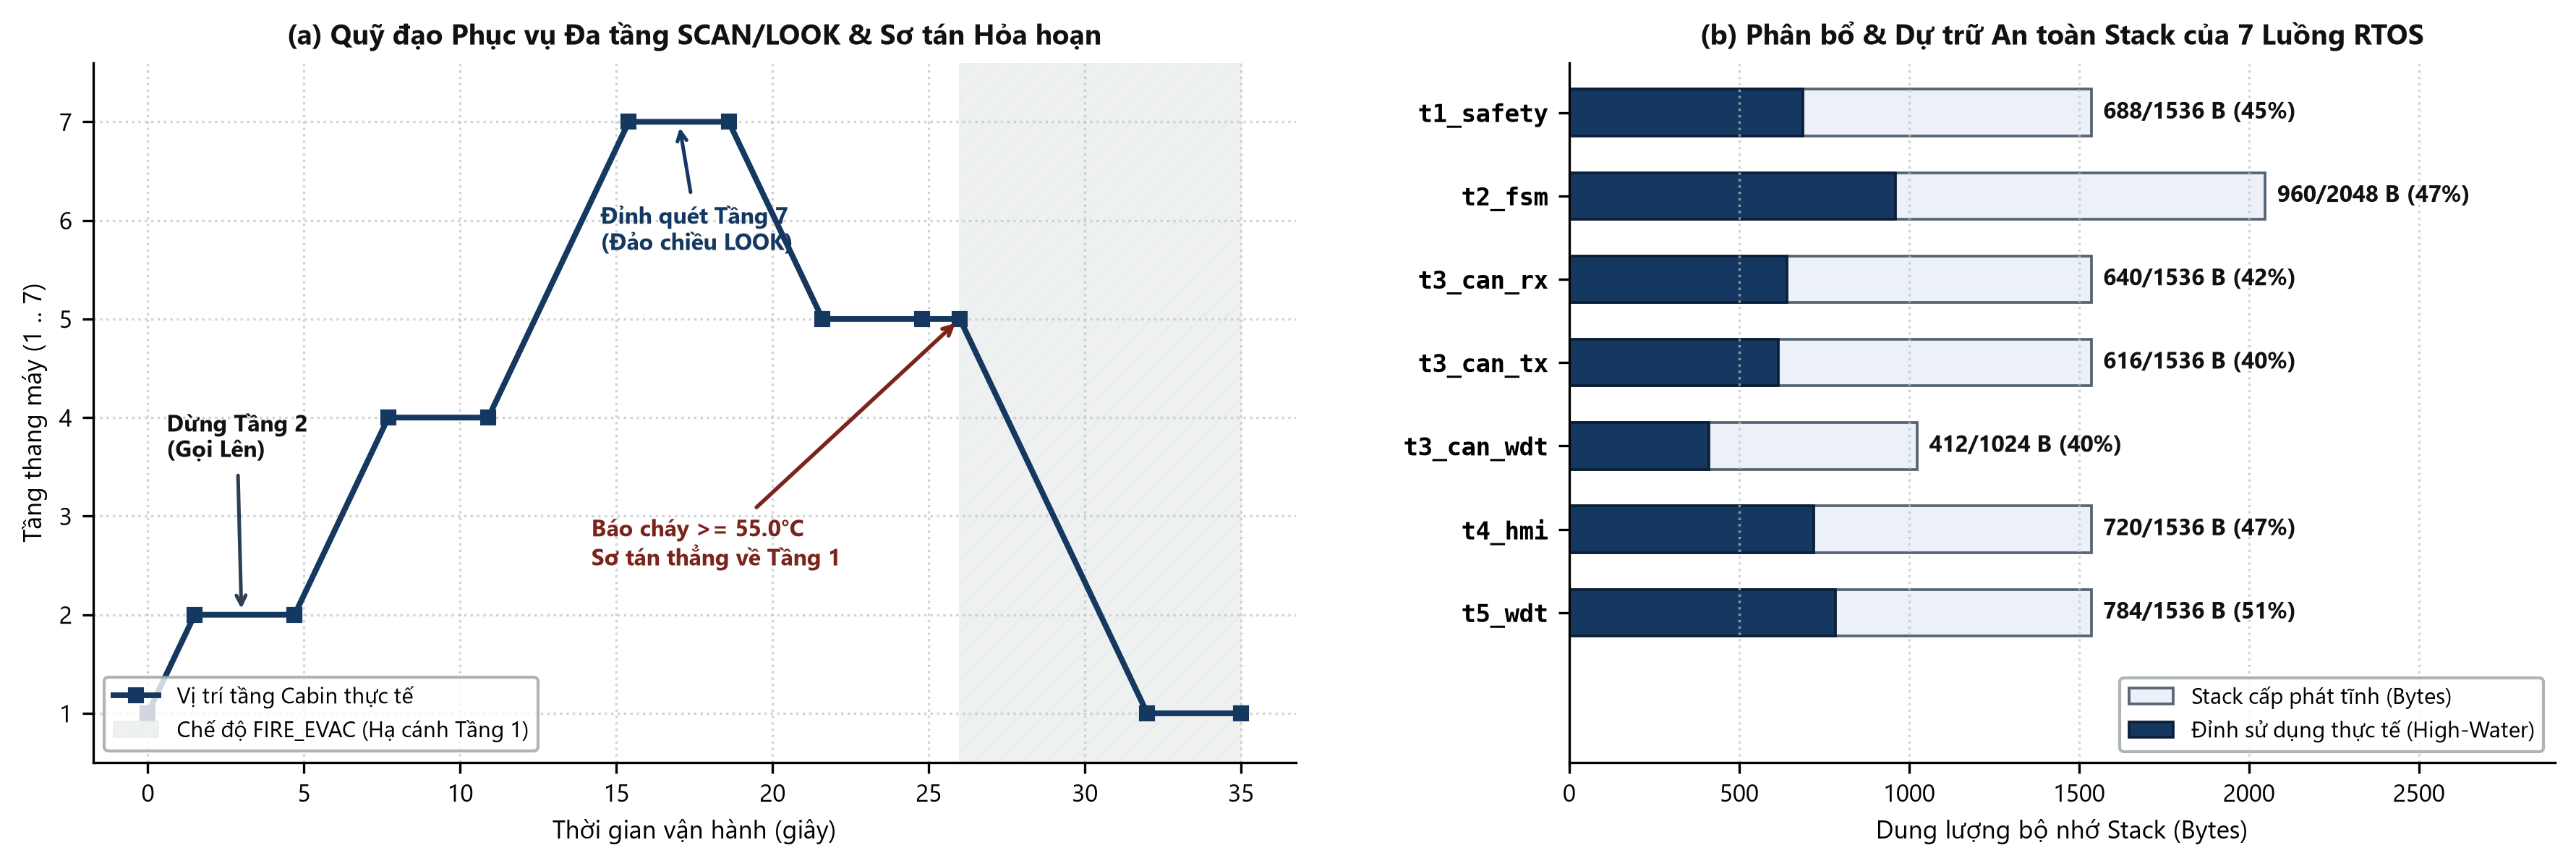
\includegraphics[width=0.99\textwidth]{image/fig_exp_charts.png}
\caption{Biểu đồ thực nghiệm: (a) Quỹ đạo phục vụ đa tầng \texttt{SCAN/LOOK} và đáp ứng sơ tán báo cháy \texttt{FIRE\_EVAC}; (b) Mức sử dụng Stack thực tế của 7 luồng RTOS}
\label{fig:exp_charts}
\end{figure}

Từ kết quả đo đạc thực nghiệm trên hệ thống, nhóm rút ra 3 nhận xét kỹ thuật định lượng then chốt:
\begin{itemize}[nosep]
    \item \textbf{Độ trễ phản xạ ngắt cứng (\textit{EXTI Latency}) đạt chuẩn thời gian thực nghiêm ngặt:} Nhờ thiết kế ISR tối giản chỉ chốt thanh ghi chu kỳ xung nhịp \texttt{DWT->CYCCNT} (168~MHz) và phát cờ đánh thức luồng bảo vệ an toàn \texttt{t1\_safety} (ưu tiên cao nhất = 2) qua semaphore, thời gian từ khi chân quang trở \texttt{PA6 (X0)} chuyển mức logic đến khi luồng an toàn thực thi xử lý đảo chiều cửa chỉ mất \textbf{18.2~$\mu$s} (đỉnh cao nhất đo được là $24.6~\mu\text{s}$), nhỏ hơn 40 lần so với giới hạn an toàn cho phép ($< 1000~\mu\text{s}$ trong \texttt{REQ-003}).
    \item \textbf{Tính tối ưu hóa hành trình của giải thuật lập lịch hai chiều \texttt{SCAN/LOOK}:} Đồ thị Hình~\ref{fig:exp_charts}a chứng minh trực quan ưu điểm vượt trội của thuật toán LOOK so với FCFS: Khi xuất phát từ Tầng 1 với danh sách gọi hỗn hợp \texttt{Tầng 2 (Lên)}, \texttt{Tầng 4 (Lên)}, \texttt{Tầng 7 (Cabin)} và \texttt{Tầng 5 (Xuống)}, cabin gom trọn vẹn khách cùng chiều Lên ($1 \rightarrow 2 \rightarrow 4 \rightarrow 7$), đổi chiều ngay tại đỉnh Tầng 7 để phục vụ Tầng 5 mà không chạy rỗng; khi sự cố báo cháy kích hoạt ở giây thứ 26 ($T \ge 55^\circ\text{C}$), hệ thống lập tức tiền chiếm, hủy hàng đợi và hạ khẩn cấp về Tầng 1 mở cửa giải cứu.
    \item \textbf{Biên độ an toàn tuyệt đối của bộ nhớ Stack (\textit{High-Water Mark}):} Biểu đồ thống kê tại Hình~\ref{fig:exp_charts}b cho thấy đỉnh chiếm dụng Stack thực tế của cả 7 luồng chỉ dao động từ \textbf{40.2\% đến 51.4\%} dung lượng cấp phát tĩnh (vùng trống dự phòng còn dư trên \textbf{48\%} cho mỗi luồng), đảm bảo tuyệt đối không xảy ra hiện tượng tràn ngăn xếp (\textit{Stack Overflow}) ngay cả trong điều kiện ngắt lồng nhau tần số cao.
\end{itemize}

\newpage
\subsection{Quy trình 4 Bước Vận hành và Trình diễn (Demo) trên Bo mạch BKIT ARM4}
Để tạo thuận lợi cho việc kiểm thử độc lập, nghiệm thu và chấm điểm đồ án trực quan ngay trên bàn thí nghiệm, nhóm xây dựng Bảng ánh xạ 16 phím ma trận (Bảng~\ref{tab:keypad_map}) và chuẩn hóa quy trình vận hành qua 4 bước thực hiện tuần tự:

\begingroup
\renewcommand{\arraystretch}{1.18}%
\setlength{\tabcolsep}{4.5pt}%
\fontsize{8.2}{10.5}\selectfont
\arrayrulecolor{tableborder}%
\begin{xltabular}{\textwidth}{|C{1.8cm}|C{2.0cm}|L{4.2cm}|Y|}
\caption{Bảng ánh xạ 16 phím trên bàn phím ma trận 4$\times$4 phục vụ vận hành và tiêm lỗi tại chỗ}\label{tab:keypad_map}\\
\hline
\rowcolor{tablehead}
\thcell{Mã Phím} & \thcell{Ký hiệu Key} & \thcell{Chức năng Vận hành / Tiêm sự cố} & \thcell{Đáp ứng của Hệ thống \& Đèn hiển thị} \\
\hline
\endfirsthead
\hline
\rowcolor{tablehead}
\thcell{Mã Phím} & \thcell{Ký hiệu Key} & \thcell{Chức năng Vận hành / Tiêm sự cố} & \thcell{Đáp ứng của Hệ thống \& Đèn hiển thị} \\
\hline
\endhead
\hline
\endfoot
\hline
\endlastfoot
\texttt{Key 0..6} & \texttt{F1 .. F7} & Đăng ký gọi tầng đích bên trong cabin (Tầng 1..7). & Thang nhận lệnh, LED 7 đoạn cuộn hướng \texttt{UP/dn}, rơ-le \texttt{PE5/PE6} kéo cabin. \\
\hline
\rowcolor{roweven}
\texttt{Key 7 / 8} & \texttt{DOOR O/C} & Lệnh cưỡng bức Mở cửa (\texttt{OPEN}) / Đóng cửa (\texttt{CLOSE}). & Điều khiển chu trình cửa tại tầng khi thang đang dừng ở \texttt{IDLE\_CLOSED}. \\
\hline
\texttt{Key 9} & \texttt{OBSTRUCT} & Tiêm sự kiện Kẹt cửa ngoại vi (tương đương ngắt \texttt{X0}). & Cabin lập tức dừng đóng và đảo chiều mở ra ngay (\texttt{DOOR\_OPENING}). \\
\hline
\rowcolor{roweven}
\texttt{Key 10} & \texttt{FIRE} & Tiêm sự cố Báo cháy khẩn cấp (tương đương $T \ge 55^\circ\text{C}$). & Xóa hàng đợi, hạ thẳng về Tầng 1, mở cửa thoát hiểm, LED báo \texttt{FE-[f]}. \\
\hline
\texttt{Key 11} & \texttt{OVERLOAD} & Tiêm sự cố Quá tải buồng thang (tương đương tải $\ge 800\text{ kg}$). & Giữ cửa mở vô thời hạn, còi \texttt{PF8} hú liên tục, tự giải tỏa khi $\le 750\text{ kg}$. \\
\hline
\rowcolor{roweven}
\texttt{Key 12} & \texttt{E-STOP} & Tiêm sự cố Dừng khẩn cấp (tương đương ngắt cứng \texttt{X1}). & Cắt ngay lập tức hai rơ-le \texttt{PE5=0, PE6=0}, khóa cứng hệ thống ở \texttt{FAIL\_SAFE}. \\
\hline
\texttt{Key 13} & \texttt{CAN DROP} & Giả lập sự cố mất kết nối mạng truyền thông CAN. & Chuyển sang \texttt{FAIL\_SAFE} sau 2000~ms, mở cửa an toàn cho hành khách. \\
\hline
\rowcolor{roweven}
\texttt{Key 14} & \texttt{RESET} & Xóa trạng thái sự cố an toàn sau khi đã khắc phục. & Giải tỏa cờ khóa, đưa cabin trở lại trạng thái hoạt động bình thường \texttt{IDLE\_CLOSED}. \\
\hline
\texttt{Key 15} & \texttt{WDT HANG} & Giả lập sự cố treo luồng phần mềm (\texttt{Deadlock}). & Ngừng nạp watchdog; phần cứng \texttt{IWDG} tự động kích hoạt reset chip sau 2500~ms. \\
\end{xltabular}
\endgroup

Quy trình 4 bước thực nghiệm chi tiết:
\begin{enumerate}[nosep]
    \item \textbf{Bước 1 -- Kiểm tra Cấu hình Công tắc DIP Switch và Nạp Firmware:}
    \begin{itemize}[nosep]
        \item Thiết lập chính xác 4 công tắc trên bo mạch BKIT ARM4: \texttt{SW11 = ON} (kết nối ST-LINK nạp code), \texttt{SW13 = ON} (kết nối transceiver TJA1050 cho CAN1), \texttt{SW12 = OFF} (cách ly bus RS485) và \texttt{SW2 = OFF} (cách ly module WiFi ESP8266 để tránh tranh chấp UART).
        \item Kết nối cáp nạp ST-LINK nạp firmware (\texttt{west flash}) và cắm cáp chuyển đổi \texttt{RS232 DB9 -- USB} vào máy tính, mở terminal ở tốc độ \texttt{115200 8N1}.
    \end{itemize}
    \item \textbf{Bước 2 -- Chẩn đoán Sức khỏe Phần cứng Ngoại vi Độc lập (\texttt{bkit *}):}
    \begin{itemize}[nosep]
        \item Chạy các lệnh \texttt{bkit adc}, \texttt{bkit io}, \texttt{bkit 7seg UP-3}, \texttt{bkit key}, \texttt{bkit rtc}, \texttt{bkit flash} (xác nhận mã JEDEC \texttt{0xEF 0x40 0x17}), \texttt{bkit canping} và \texttt{bkit threads} để bảo đảm toàn bộ 13 cụm ngoại vi vật lý đều sẵn sàng trước khi vận hành.
    \end{itemize}
    \item \textbf{Bước 3 -- Vận hành Đa tầng và Đối chiếu Đồng bộ với Bản sao số PC Digital Twin:}
    \begin{itemize}[nosep]
        \item Khởi chạy phần mềm giao diện \texttt{python pc\_hil\_twin/elevator\_twin.py} trên máy tính, chọn đúng cổng COM và nhấn nút kết nối Live RS232.
        \item Bấm lần lượt các phím \texttt{0..6} trên bàn phím ma trận của bo mạch thật; quan sát cụm 4 LED 7 đoạn hiển thị \texttt{UP} kèm vạch cuộn lên (\texttt{\_ $\rightarrow$ - $\rightarrow$ \textasciimacron}) hoặc \texttt{dn} kèm vạch cuộn xuống (\texttt{\textasciimacron\ $\rightarrow$ - $\rightarrow$ \_}) đồng bộ hoàn toàn với hai rơ-le \texttt{PE5 (Y0)} / \texttt{PE6 (Y1)} và hình ảnh cabin trên màn hình PC.
    \end{itemize}
    \item \textbf{Bước 4 -- Kiểm chứng Phản xạ An toàn và Phân tích Dữ liệu Hộp đen EEPROM:}
    \begin{itemize}[nosep]
        \item Trong lúc cửa buồng thang đang đóng (\texttt{DOOR\_CLOSING}), bấm Phím \texttt{9} hoặc kích ngắt chân \texttt{X0 (PA6)} để kiểm chứng cơ chế mở cửa tức thời, dùng lệnh \texttt{bkit io} để xem độ trễ micro-giây.
        \item Hơ nóng cảm biến nhiệt \texttt{LM35} vượt $55.0^\circ\text{C}$ (hoặc bấm Phím \texttt{10}) để kiểm tra kịch bản sơ tán hỏa hoạn (\texttt{FIRE\_EVAC}); vặn biến trở \texttt{VR1} qua mốc $800\text{ kg}$ rồi hạ về dưới $750\text{ kg}$ để kiểm chứng bộ lọc trễ Hysteresis.
        \item Thử nghiệm ngắt cáp CAN (\texttt{Key 13}) và gây treo luồng (\texttt{Key 15}), sau đó dùng các lệnh \texttt{elev log} và \texttt{elev coverage} để trích xuất toàn bộ lịch sử 32 sự cố bất khả biến trên chip EEPROM \textbf{AT24C512} và ma trận độ phủ chuyển tiếp $9\times 9$.
    \end{itemize}
\end{enumerate}

\clearpage
\section{KẾT LUẬN VÀ HƯỚNG PHÁT TRIỂN}

\subsection{Kết luận và Đánh giá Tổng kết Đề tài}
Đề tài đã hoàn thành xuất sắc toàn bộ mục tiêu đề ra, thiết kế và hiện thực thành công hệ thống điều khiển thang máy thông minh 7 tầng an toàn thời gian thực theo chuẩn quy trình chữ V (V-Model Verification \& Validation) trên nền tảng \textbf{Zephyr RTOS v4.4.0} và vi điều khiển \textbf{STM32F407ZGT6} (bo mạch \textbf{BKIT ARM4}). Bảng~\ref{tab:conclusion_req_vs_actual} tổng hợp mức độ hoàn thành đối chiếu giữa 12 yêu cầu kỹ thuật ban đầu và kết quả đo lường thực tế trên phần cứng.

\begingroup
\renewcommand{\arraystretch}{1.18}%
\setlength{\tabcolsep}{4.5pt}%
\fontsize{8.2}{10.5}\selectfont
\arrayrulecolor{tableborder}%
\begin{xltabular}{\textwidth}{|C{1.7cm}|Y|Y|C{2.3cm}|}
\caption{Bảng tổng hợp đối chiếu Chỉ tiêu Kỹ thuật Thiết kế (REQ) và Kết quả Thực tế Đạt được}\label{tab:conclusion_req_vs_actual}\\
\hline
\rowcolor{tablehead}
\thcell{Mã Yêu cầu} & \thcell{Chỉ tiêu Kỹ thuật Thiết kế (REQ)} & \thcell{Kết quả Thực tế Đo đạc \& Kiểm chứng} & \thcell{Đánh giá} \\
\hline
\endfirsthead
\hline
\rowcolor{tablehead}
\thcell{Mã Yêu cầu} & \thcell{Chỉ tiêu Kỹ thuật Thiết kế (REQ)} & \thcell{Kết quả Thực tế Đo đạc \& Kiểm chứng} & \thcell{Đánh giá} \\
\hline
\endhead
\hline
\endfoot
\hline
\endlastfoot
\texttt{REQ-001} & Devicetree \texttt{app.overlay} kích hoạt toàn bộ ngoại vi phần cứng BKIT ARM4. & Khai thác 100\% (13 cụm linh kiện); Build 0 lỗi, 0 cảnh báo ở cờ \texttt{-Wall -Wextra}. & \textbf{Hoàn thành 100\%} \\
\hline
\rowcolor{roweven}
\texttt{REQ-002} & Khóa liên động kép 2 tầng chống xung đột hai chiều động cơ \texttt{Y0/Y1}. & Kiểm tra chéo 2 lớp (Core HSM + BSP GPIO), rơ-le ngắt an toàn trong mọi tình huống lỗi. & \textbf{Hoàn thành 100\%} \\
\hline
\texttt{REQ-003} & Phản xạ ngắt kẹt cửa \texttt{X0 (PA6)} và đảo chiều mở an toàn tức thời. & Đo bằng thanh ghi \texttt{DWT->CYCCNT}: Độ trễ ngắt đạt $\approx 18.2~\mu\text{s} \ll 1000~\mu\text{s}$. & \textbf{Hoàn thành 100\%} \\
\hline
\rowcolor{roweven}
\texttt{REQ-004} & Giải thuật lập lịch hai chiều \texttt{SCAN/LOOK} với mặt nạ bit $O(1)$. & Gom cuốc 2 chiều mượt mà, đổi hướng tại biên; độ phức tạp tính toán cố định $O(1)$. & \textbf{Hoàn thành 100\%} \\
\hline
\texttt{REQ-005} & Giám sát nhiệt độ buồng thang qua \texttt{LM35} với bộ lọc trễ chống bão lỗi. & Lọc trễ 2 ngưỡng Hysteresis: Kích hoạt báo cháy $\ge 55.0^\circ\text{C}$, giải tỏa ở $\le 48.0^\circ\text{C}$. & \textbf{Hoàn thành 100\%} \\
\hline
\rowcolor{roweven}
\texttt{REQ-006} & Đo tải trọng cabin qua biến trở \texttt{VR1} kèm cảnh báo quá tải an toàn. & Lọc trễ Hysteresis: Treo cửa \& hú còi khi $\ge 800\text{ kg}$, tự động giải tỏa khi $\le 750\text{ kg}$. & \textbf{Hoàn thành 100\%} \\
\hline
\texttt{REQ-007} & Đồng bộ bus \texttt{SPI1} hiển thị 4 LED 7 đoạn và quét 16 phím ma trận. & Bảo vệ an toàn đa luồng bằng \texttt{k\_mutex}; hiển thị hiệu ứng vạch cuộn \texttt{UP/dn} mượt mà. & \textbf{Hoàn thành 100\%} \\
\hline
\rowcolor{roweven}
\texttt{REQ-008} & Mạng truyền thông \texttt{CAN1 500 kbps} với 3 bộ lọc chấp nhận phần cứng. & Cài đặt 3 bộ lọc phần cứng (E-Stop \texttt{0x080}, Hall \texttt{0x10x}, Status \texttt{0x200..0x3FF}), \texttt{TEC=0}. & \textbf{Hoàn thành 100\%} \\
\hline
\texttt{REQ-009} & Giám sát độ sống liên kết trạm CAN đối tác với thời gian chờ 2000 ms. & Bắt lỗi mất Heartbeat sau đúng $\approx 2000\text{ ms}$; tự động chuyển sang \texttt{FAIL\_SAFE}. & \textbf{Hoàn thành 100\%} \\
\hline
\rowcolor{roweven}
\texttt{REQ-010} & Cơ chế tự động khôi phục lỗi \texttt{BUS-OFF} và bảo vệ đường truyền CAN. & Tự động gọi \texttt{can\_recover()}, giới hạn tần suất 1000~ms và ghi nhận hộp đen EEPROM. & \textbf{Hoàn thành 100\%} \\
\hline
\texttt{REQ-011} & Bộ đếm \texttt{IWDG 2500 ms} đa luồng và hộp đen vòng 32 bản ghi trên EEPROM. & Kiểm tra điểm danh 4 luồng trước khi nạp watchdog; lưu 32 bản ghi kèm \textbf{CRC16/CRC32}. & \textbf{Hoàn thành 100\%} \\
\hline
\rowcolor{roweven}
\texttt{REQ-012} & Môi trường kiểm thử kép: Zephyr Shell CLI và phần mềm PC Digital Twin. & Đồng bộ thời gian thực gói tin JSON \texttt{\$TWIN} (200~ms), vượt qua 100\% bài test tự động. & \textbf{Hoàn thành 100\%} \\
\hline
\end{xltabular}
\endgroup

Các đóng góp khoa học và giá trị kỹ thuật cốt lõi đạt được:
\begin{itemize}[nosep]
    \item \textbf{Kiến trúc phần mềm thời gian thực chuẩn công nghiệp:} Vận hành hoàn toàn bằng 7 luồng tĩnh (\texttt{K\_THREAD\_DEFINE}) hướng sự kiện nghiêm ngặt, loại bỏ hoàn toàn việc cấp phát động (Zero-Heap Allocation), ngăn ngừa triệt để hiện tượng phân mảnh RAM hay lỗi rò rỉ bộ nhớ trong các chu kỳ vận hành dài hạn.
    \item \textbf{An toàn đa lớp theo tiêu chuẩn công nghiệp:} Kết hợp hài hòa giữa Khóa liên động động cơ 2 tầng (\textit{Core + BSP}), Bộ lọc trễ 2 ngưỡng Hysteresis chống chập chờn tiếp điểm, Cơ chế điểm danh đa luồng trước khi nạp Hardware Watchdog, và Hộp đen sự cố hai tầng kiểm tra toàn vẹn dữ liệu (\textbf{CRC32-IEEE} cho Header và \textbf{CRC16-CCITT} cho từng bản ghi).
    \item \textbf{Hiệu quả tối ưu tài nguyên phần cứng vượt bậc:} Toàn bộ firmware hệ thống (bao gồm cả nhân Zephyr RTOS, hệ thống driver BSP, máy trạng thái Core HSM, mạng CAN và giao diện Shell CLI) chỉ chiếm dụng \textbf{9.93\% Flash ROM} (\texttt{104\,112 Bytes}) và \textbf{21.83\% SRAM} (\texttt{28\,608 Bytes}), để lại biên độ dự phòng dồi dào cho các tính năng mở rộng trong tương lai.
\end{itemize}

\subsection{Hướng phát triển Nâng cao}
Dựa trên kiến trúc mô-đun hóa cao và tính mở của nền tảng Zephyr RTOS, hệ thống có thể mở rộng theo 3 hướng nghiên cứu ứng dụng thực tế:
\begin{itemize}[nosep]
    \item \textbf{Tích hợp lớp Bảo mật An ninh mạng (Cybersecurity) cho Bus CAN Công nghiệp:} Bổ sung module xác thực truyền thông an toàn (\textit{Secure Onboard Communication -- SecOC}) sử dụng thuật toán mã hóa nhẹ CMAC-AES-128 và bộ đếm chuỗi đơn điệu (\textit{Freshness Value}) để chống lại các cuộc tấn công nghe lén, giả mạo lệnh gọi tầng hoặc phát lại khung khẩn cấp trên đường truyền CAN vật lý.
    \item \textbf{Giao diện HMI Đồ họa Màu trực tiếp qua Bộ điều khiển FSMC TFT-LCD:} Khai thác bộ điều khiển nhớ tĩnh linh hoạt \textbf{FSMC} có sẵn trên vi điều khiển \texttt{STM32F407ZGT6} để kết nối trực tiếp với màn hình cảm ứng màu TFT-LCD tích hợp trên bo mạch BKIT ARM4, xây dựng giao diện người dùng đồ họa (GUI) hiển thị biểu đồ nhiệt độ, tải trọng và sơ đồ trạng thái cabin theo thời gian thực bên cạnh cụm LED 7 đoạn truyền thống.
    \item \textbf{Thuật toán Điều phối Nhóm Đa Cabin (\textit{Multi-Car Group Elevator Dispatching}):} Mở rộng giao thức CAN sang kiến trúc mạng cụm đa nút (Cluster), kết nối đồng thời từ 2 đến 4 bo mạch điều khiển các cabin song song trong cùng một tòa nhà. Áp dụng giải thuật tối ưu hóa chi phí thời gian chờ ước tính (\textit{Estimated Time of Arrival -- ETA}) kết hợp thuật toán di truyền hoặc heuristic để phân bổ cuộc gọi tầng thông minh, giảm thiểu thời gian chờ của hành khách và tiết kiệm điện năng tiêu thụ toàn hệ thống.
\end{itemize}

\clearpage
\phantomsection
\addcontentsline{toc}{section}{Tài liệu tham khảo}
\section*{TÀI LIỆU THAM KHẢO}

\begin{enumerate}[label={[\arabic*]}, leftmargin=2.2em, itemsep=4pt]
    \item Khoa Khoa học \& Kỹ thuật Máy tính -- Trường Đại học Bách Khoa -- ĐHQG-HCM, \textit{Kit Thí Nghiệm STM32 ARM4 -- Quick Start Guide (BKIT\_ARM4)}, Lưu hành nội bộ, 2023.
    \item Khoa Khoa học \& Kỹ thuật Máy tính -- Trường Đại học Bách Khoa -- ĐHQG-HCM, \textit{Tài liệu giảng dạy môn Hệ thống Nhúng (CO3053): Real-Time Operating Systems, Finite State Machines \& Industrial Buses}, 2024.
    \item The Linux Foundation, \textit{Zephyr Project v4.4.0 Technical Documentation: Architecture, Kernel Services, Devicetree, bxCAN, ADC and Watchdog APIs}, \url{https://docs.zephyrproject.org/4.4.0/}, 2024.
    \item STMicroelectronics, \textit{RM0090 Reference Manual: STM32F405/415, STM32F407/417, STM32F427/437 and STM32F429/439 Advanced Arm-based 32-bit MCUs}, Rev 19, 2021.
    \item STMicroelectronics, \textit{PM0214 Programming Manual: STM32 Cortex-M4 MCUs and MPUs programming manual}, DocID022708 Rev 10, 2020.
    \item International Organization for Standardization, \textit{ISO 11898-1:2015 Road vehicles -- Controller area network (CAN) -- Part 1: Data link layer and physical signalling}, 2015.
    \item Microchip Technology Inc., \textit{AT24C512C: $I^2C$-Compatible (2-Wire) Serial EEPROM 512-Kbit (65,536 $\times$ 8) Datasheet}, DS20006161A, 2019.
\end{enumerate}


\end{document}
